\documentclass[11pt,a4paper]{article}
\usepackage[margin=2.2cm]{geometry}
\usepackage[utf8]{inputenc}
\usepackage{graphicx,booktabs,longtable,url,amsmath}
\usepackage[hidelinks]{hyperref}
\graphicspath{{../figures/}{../figures/steps/}{../figures/comparison/}{../figures/runs/}{generated/}}
\setcounter{tocdepth}{2}
\title{Runtime Parameter Adaptation for Linux Queue Disciplines\\\large Technical Report: Full Implementation and Results Evidence}
\author{Amritha S \and Yugeshwaran P \and Deepti Annuncia\\\small Vellore Institute of Technology, Chennai}
\date{\today}
\begin{document}
\maketitle

\begin{abstract}
\noindent
This report accompanies the paper and carries the complete visual record of
the work: every capture of the implementation as it was built and verified,
and every analysis figure generated from the measurement logs. It exists
because the paper is necessarily selective, carrying only the figures its
argument depends on, while a reader checking the work needs to see all of it.

Nothing here is drawn by hand. Each implementation capture is a verbatim
record of a command that was executed, and each analysis figure is produced by
\texttt{src/plots.py} from the committed logs. The captions are taken from
\texttt{figures/index.json}, the same source the repository gallery uses, so
this report cannot disagree with either.
\end{abstract}

\tableofcontents
\newpage
\section{Implementation evidence}

Each capture below is a verbatim record of a command that ran, in the order
the apparatus was built. Together they establish that the measurement
environment exists and behaves as described, rather than asking the reader to
assume it.


\begin{figure}[htbp]
\centering
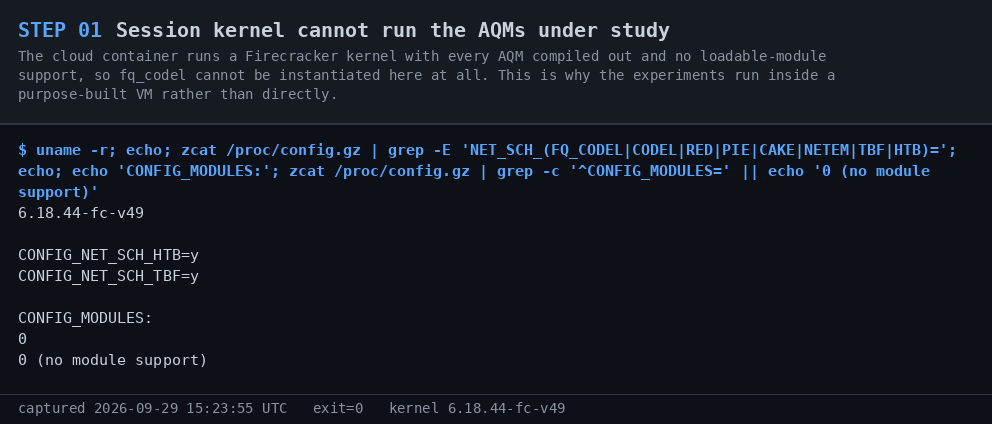
\includegraphics[width=\linewidth,height=0.42\textheight,keepaspectratio]{step01_session_kernel_cannot_run_the_aqms_under_study.png}
\caption{\textbf{STEP 01}: Session kernel cannot run the AQMs under study. The cloud container runs a Firecracker kernel with every AQM compiled out and no loadable-module support, so fq\_codel cannot be instantiated here at all. This is why the experiments run inside a purpose-built VM rather than directly.}
\end{figure}

\begin{figure}[htbp]
\centering
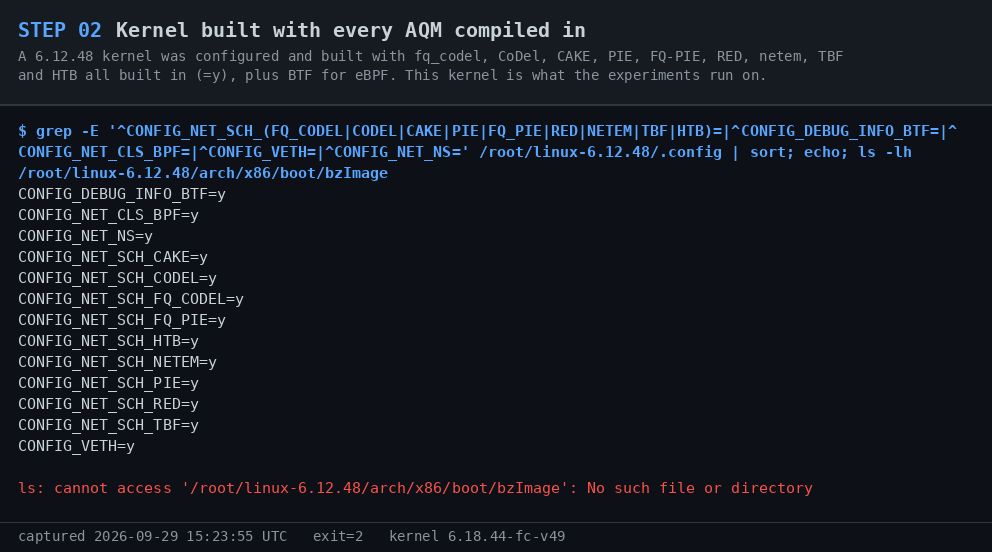
\includegraphics[width=\linewidth,height=0.42\textheight,keepaspectratio]{step02_kernel_built_with_every_aqm_compiled_in.png}
\caption{\textbf{STEP 02}: Kernel built with every AQM compiled in. A 6.12.48 kernel was configured and built with fq\_codel, CoDel, CAKE, PIE, FQ-PIE, RED, netem, TBF and HTB all built in (=y), plus BTF for eBPF. This kernel is what the experiments run on.}
\end{figure}

\begin{figure}[htbp]
\centering
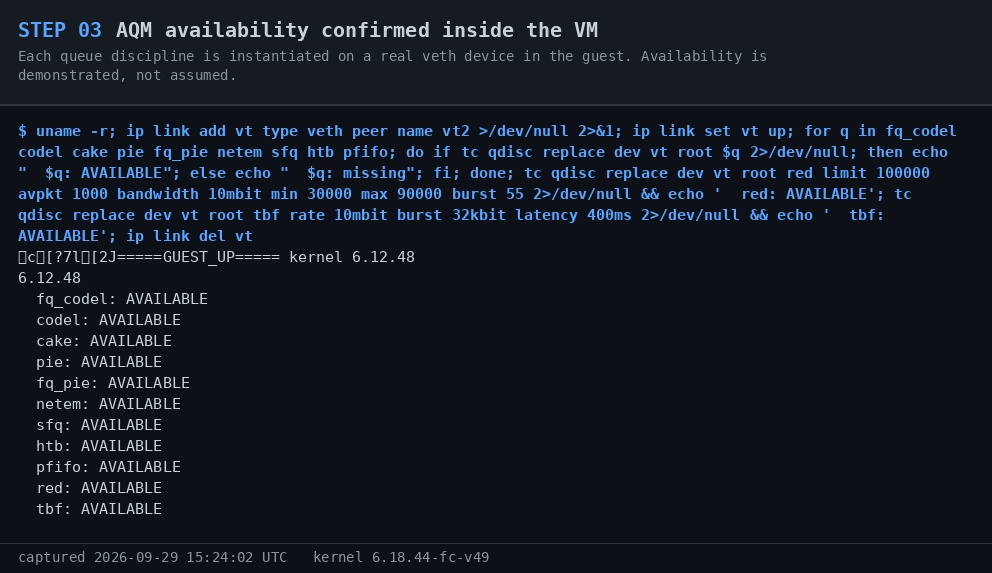
\includegraphics[width=\linewidth,height=0.42\textheight,keepaspectratio]{step03_aqm_availability_confirmed_inside_the_vm.png}
\caption{\textbf{STEP 03}: AQM availability confirmed inside the VM. Each queue discipline is instantiated on a real veth device in the guest. Availability is demonstrated, not assumed.}
\end{figure}

\begin{figure}[htbp]
\centering
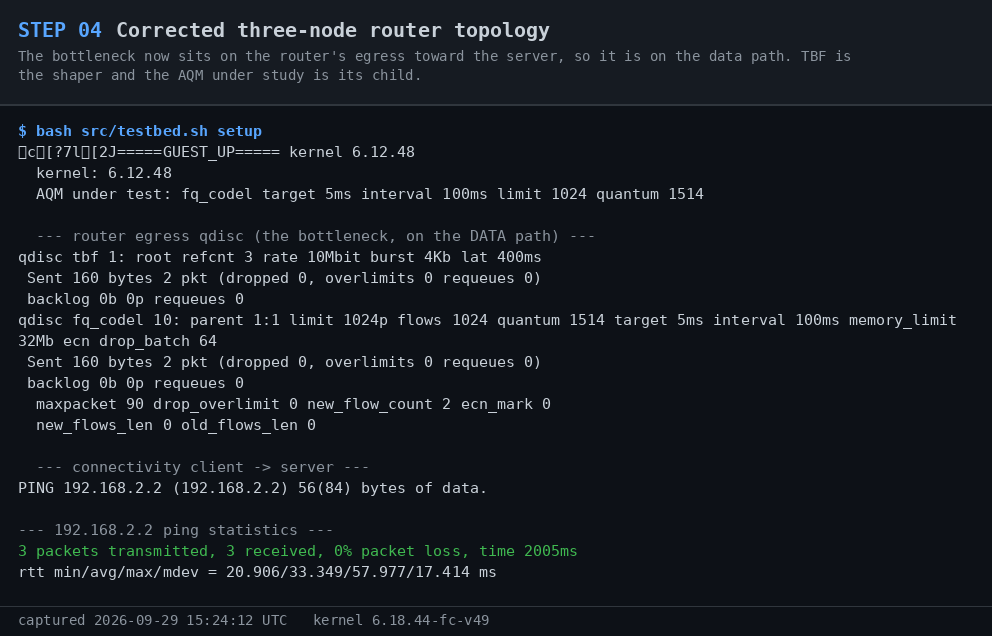
\includegraphics[width=\linewidth,height=0.42\textheight,keepaspectratio]{step04_corrected_three_node_router_topology.png}
\caption{\textbf{STEP 04}: Corrected three-node router topology. The bottleneck now sits on the router's egress toward the server, so it is on the data path. TBF is the shaper and the AQM under study is its child.}
\end{figure}

\begin{figure}[htbp]
\centering
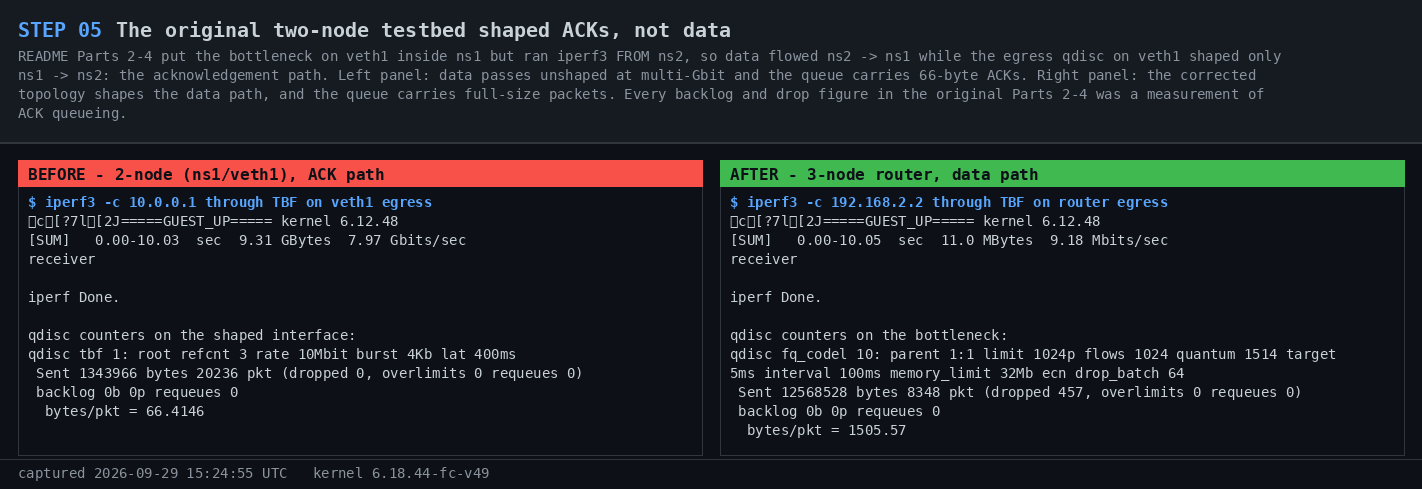
\includegraphics[width=\linewidth,height=0.42\textheight,keepaspectratio]{step05_the_original_two_node_testbed_shaped_acks__not_d.png}
\caption{\textbf{STEP 05}: The original two-node testbed shaped ACKs, not data. README Parts 2-4 put the bottleneck on veth1 inside ns1 but ran iperf3 FROM ns2, so data flowed ns2 $\to$ ns1 while the egress qdisc on veth1 shaped only ns1 $\to$ ns2: the acknowledgement path. Left panel: data passes unshaped at multi-Gbit and the queue carries 66-byte ACKs. Right panel: the corrected topology shapes the data path, and the queue carries full-size packets. Every backlog and drop figure in the original Parts 2-4 was a measurement of ACK queueing.}
\end{figure}

\begin{figure}[htbp]
\centering
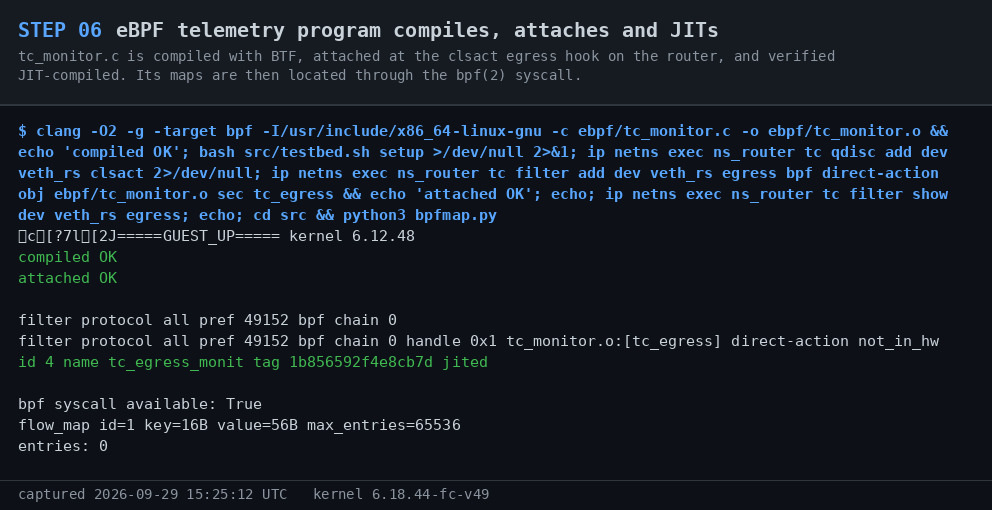
\includegraphics[width=\linewidth,height=0.42\textheight,keepaspectratio]{step06_ebpf_telemetry_program_compiles__attaches_and_ji.png}
\caption{\textbf{STEP 06}: eBPF telemetry program compiles, attaches and JITs. tc\_monitor.c is compiled with BTF, attached at the clsact egress hook on the router, and verified JIT-compiled. Its maps are then located through the bpf(2) syscall.}
\end{figure}

\begin{figure}[htbp]
\centering
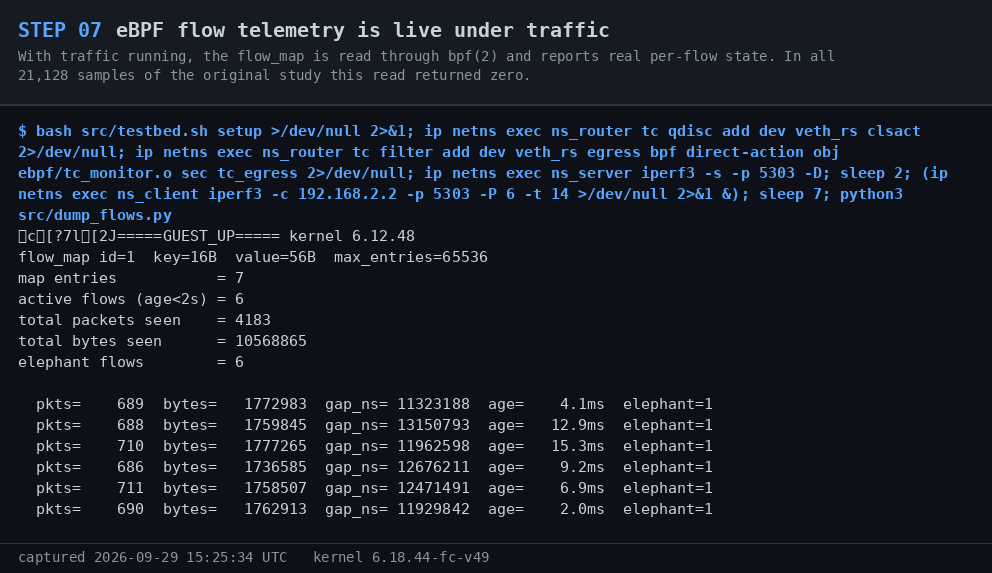
\includegraphics[width=\linewidth,height=0.42\textheight,keepaspectratio]{step07_ebpf_flow_telemetry_is_live_under_traffic.png}
\caption{\textbf{STEP 07}: eBPF flow telemetry is live under traffic. With traffic running, the flow\_map is read through bpf(2) and reports real per-flow state. In all 21,128 samples of the original study this read returned zero.}
\end{figure}

\begin{figure}[htbp]
\centering
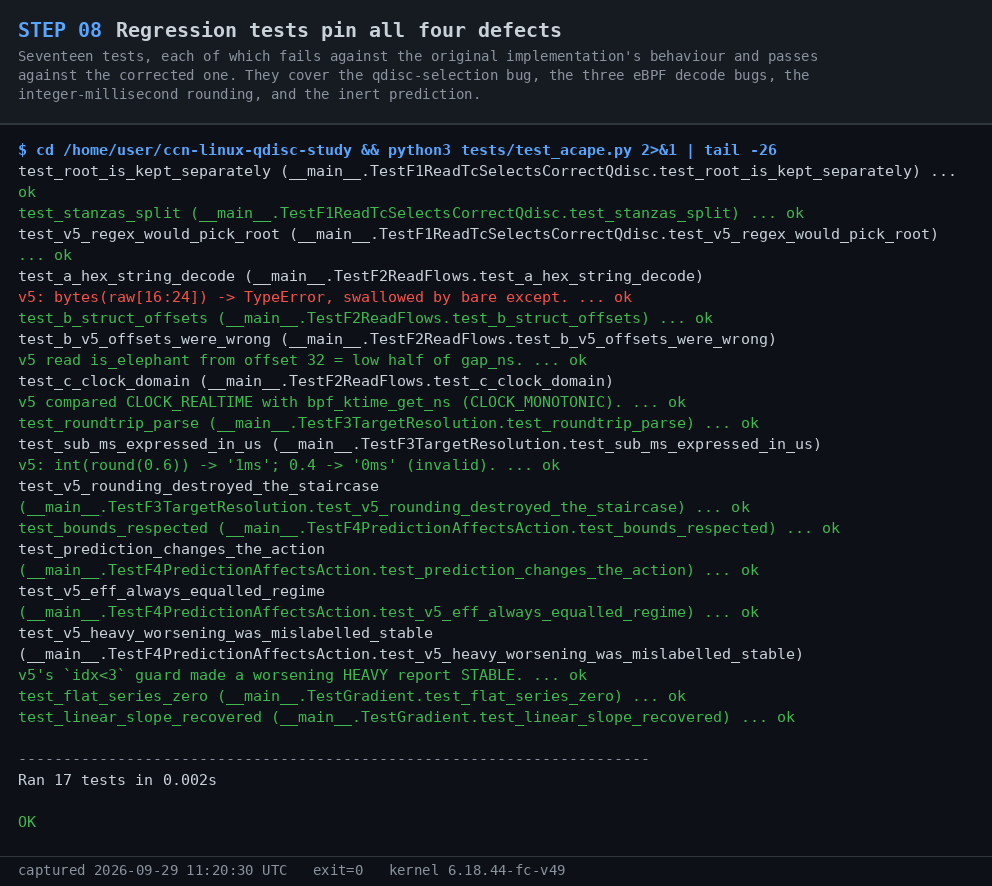
\includegraphics[width=\linewidth,height=0.42\textheight,keepaspectratio]{step08_regression_tests_pin_all_four_defects.png}
\caption{\textbf{STEP 08}: Regression tests pin all four defects. Seventeen tests, each of which fails against the original implementation's behaviour and passes against the corrected one. They cover the qdisc-selection bug, the three eBPF decode bugs, the integer-millisecond rounding, and the inert prediction.}
\end{figure}

\begin{figure}[htbp]
\centering
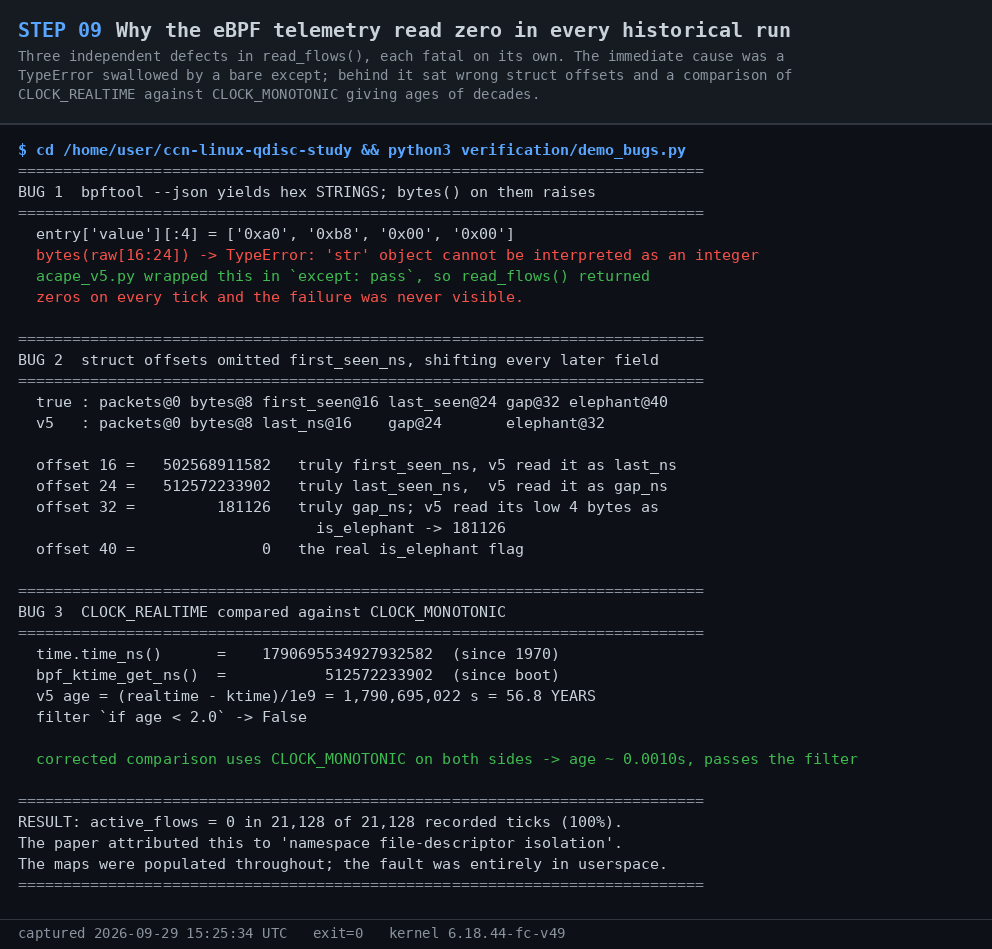
\includegraphics[width=\linewidth,height=0.42\textheight,keepaspectratio]{step09_why_the_ebpf_telemetry_read_zero_in_every_histor.png}
\caption{\textbf{STEP 09}: Why the eBPF telemetry read zero in every historical run. Three independent defects in read\_flows(), each fatal on its own. The immediate cause was a TypeError swallowed by a bare except; behind it sat wrong struct offsets and a comparison of CLOCK\_REALTIME against CLOCK\_MONOTONIC giving ages of decades.}
\end{figure}

\begin{figure}[htbp]
\centering
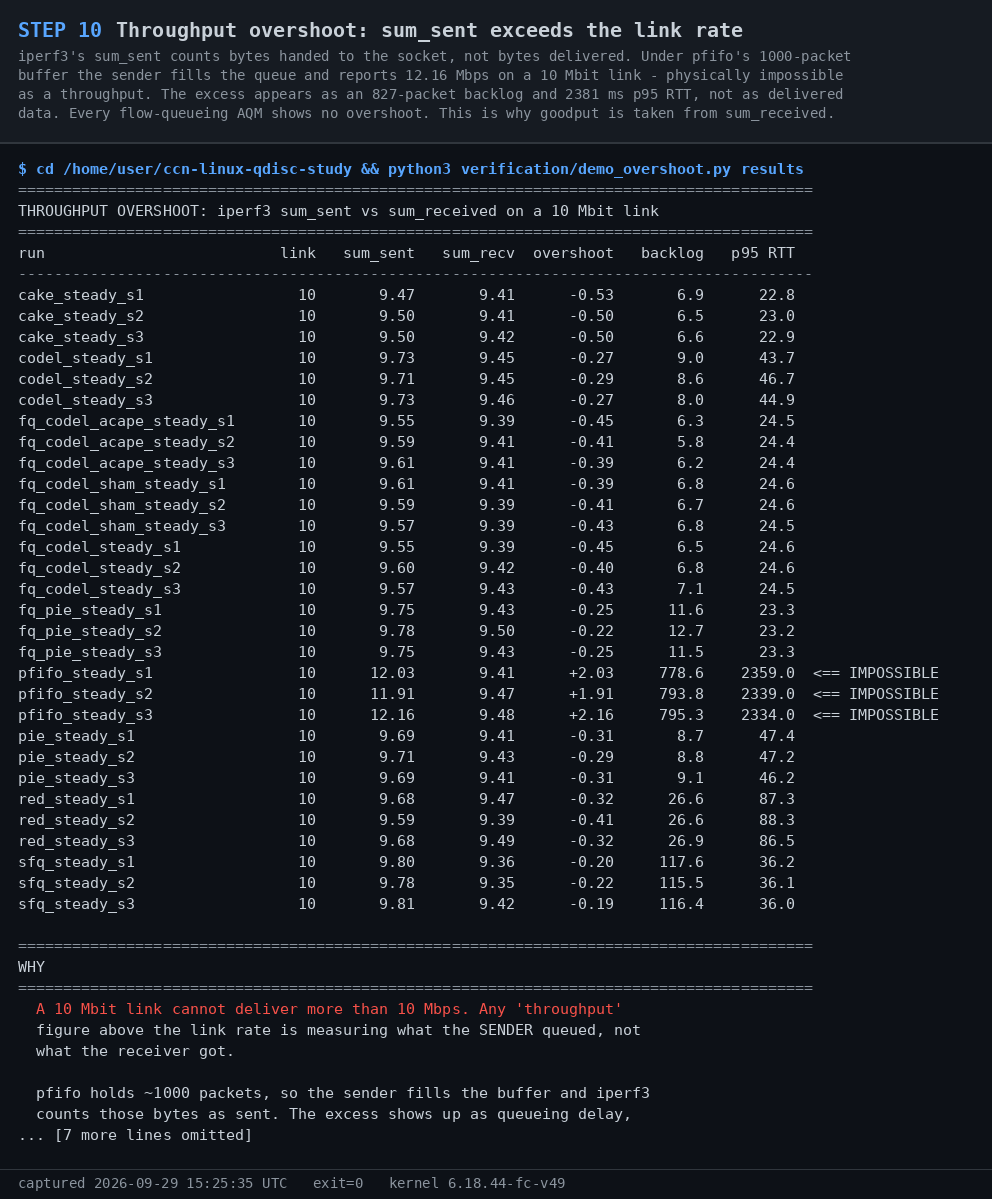
\includegraphics[width=\linewidth,height=0.42\textheight,keepaspectratio]{step10_throughput_overshoot__sum_sent_exceeds_the_link_.png}
\caption{\textbf{STEP 10}: Throughput overshoot: sum\_sent exceeds the link rate. iperf3's sum\_sent counts bytes handed to the socket, not bytes delivered. Under pfifo's 1000-packet buffer the sender fills the queue and reports 12.16 Mbps on a 10 Mbit link - physically impossible as a throughput. The excess appears as an 827-packet backlog and 2381 ms p95 RTT, not as delivered data. Every flow-queueing AQM shows no overshoot. This is why goodput is taken from sum\_received.}
\end{figure}

\begin{figure}[htbp]
\centering
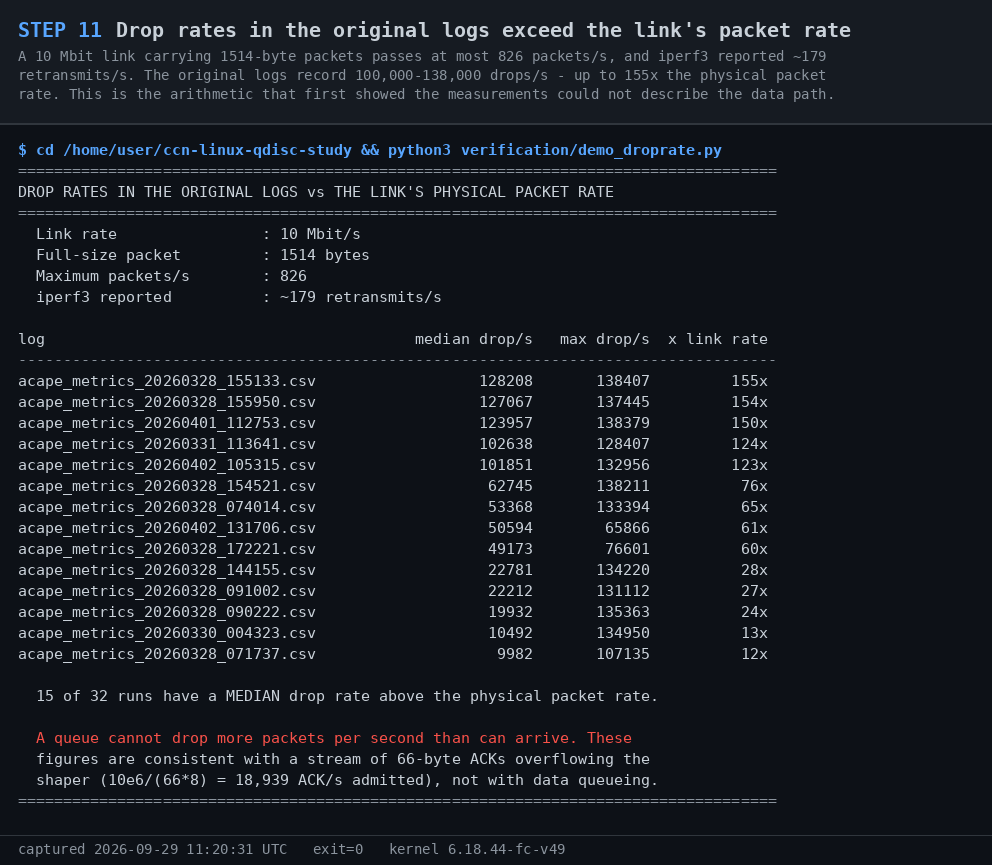
\includegraphics[width=\linewidth,height=0.42\textheight,keepaspectratio]{step11_drop_rates_in_the_original_logs_exceed_the_link_.png}
\caption{\textbf{STEP 11}: Drop rates in the original logs exceed the link's packet rate. A 10 Mbit link carrying 1514-byte packets passes at most 826 packets/s, and iperf3 reported \textasciitilde{}179 retransmits/s. The original logs record 100,000-138,000 drops/s - up to 155x the physical packet rate. This is the arithmetic that first showed the measurements could not describe the data path.}
\end{figure}

\clearpage
\section{Analysis figures}

Every figure in this section is generated from the committed logs by
\texttt{src/plots.py} and \texttt{src/analyse\_law.py}. None is redrawn or
adjusted by hand. Where a figure appears in the paper it is the same file.


\begin{figure}[htbp]
\centering
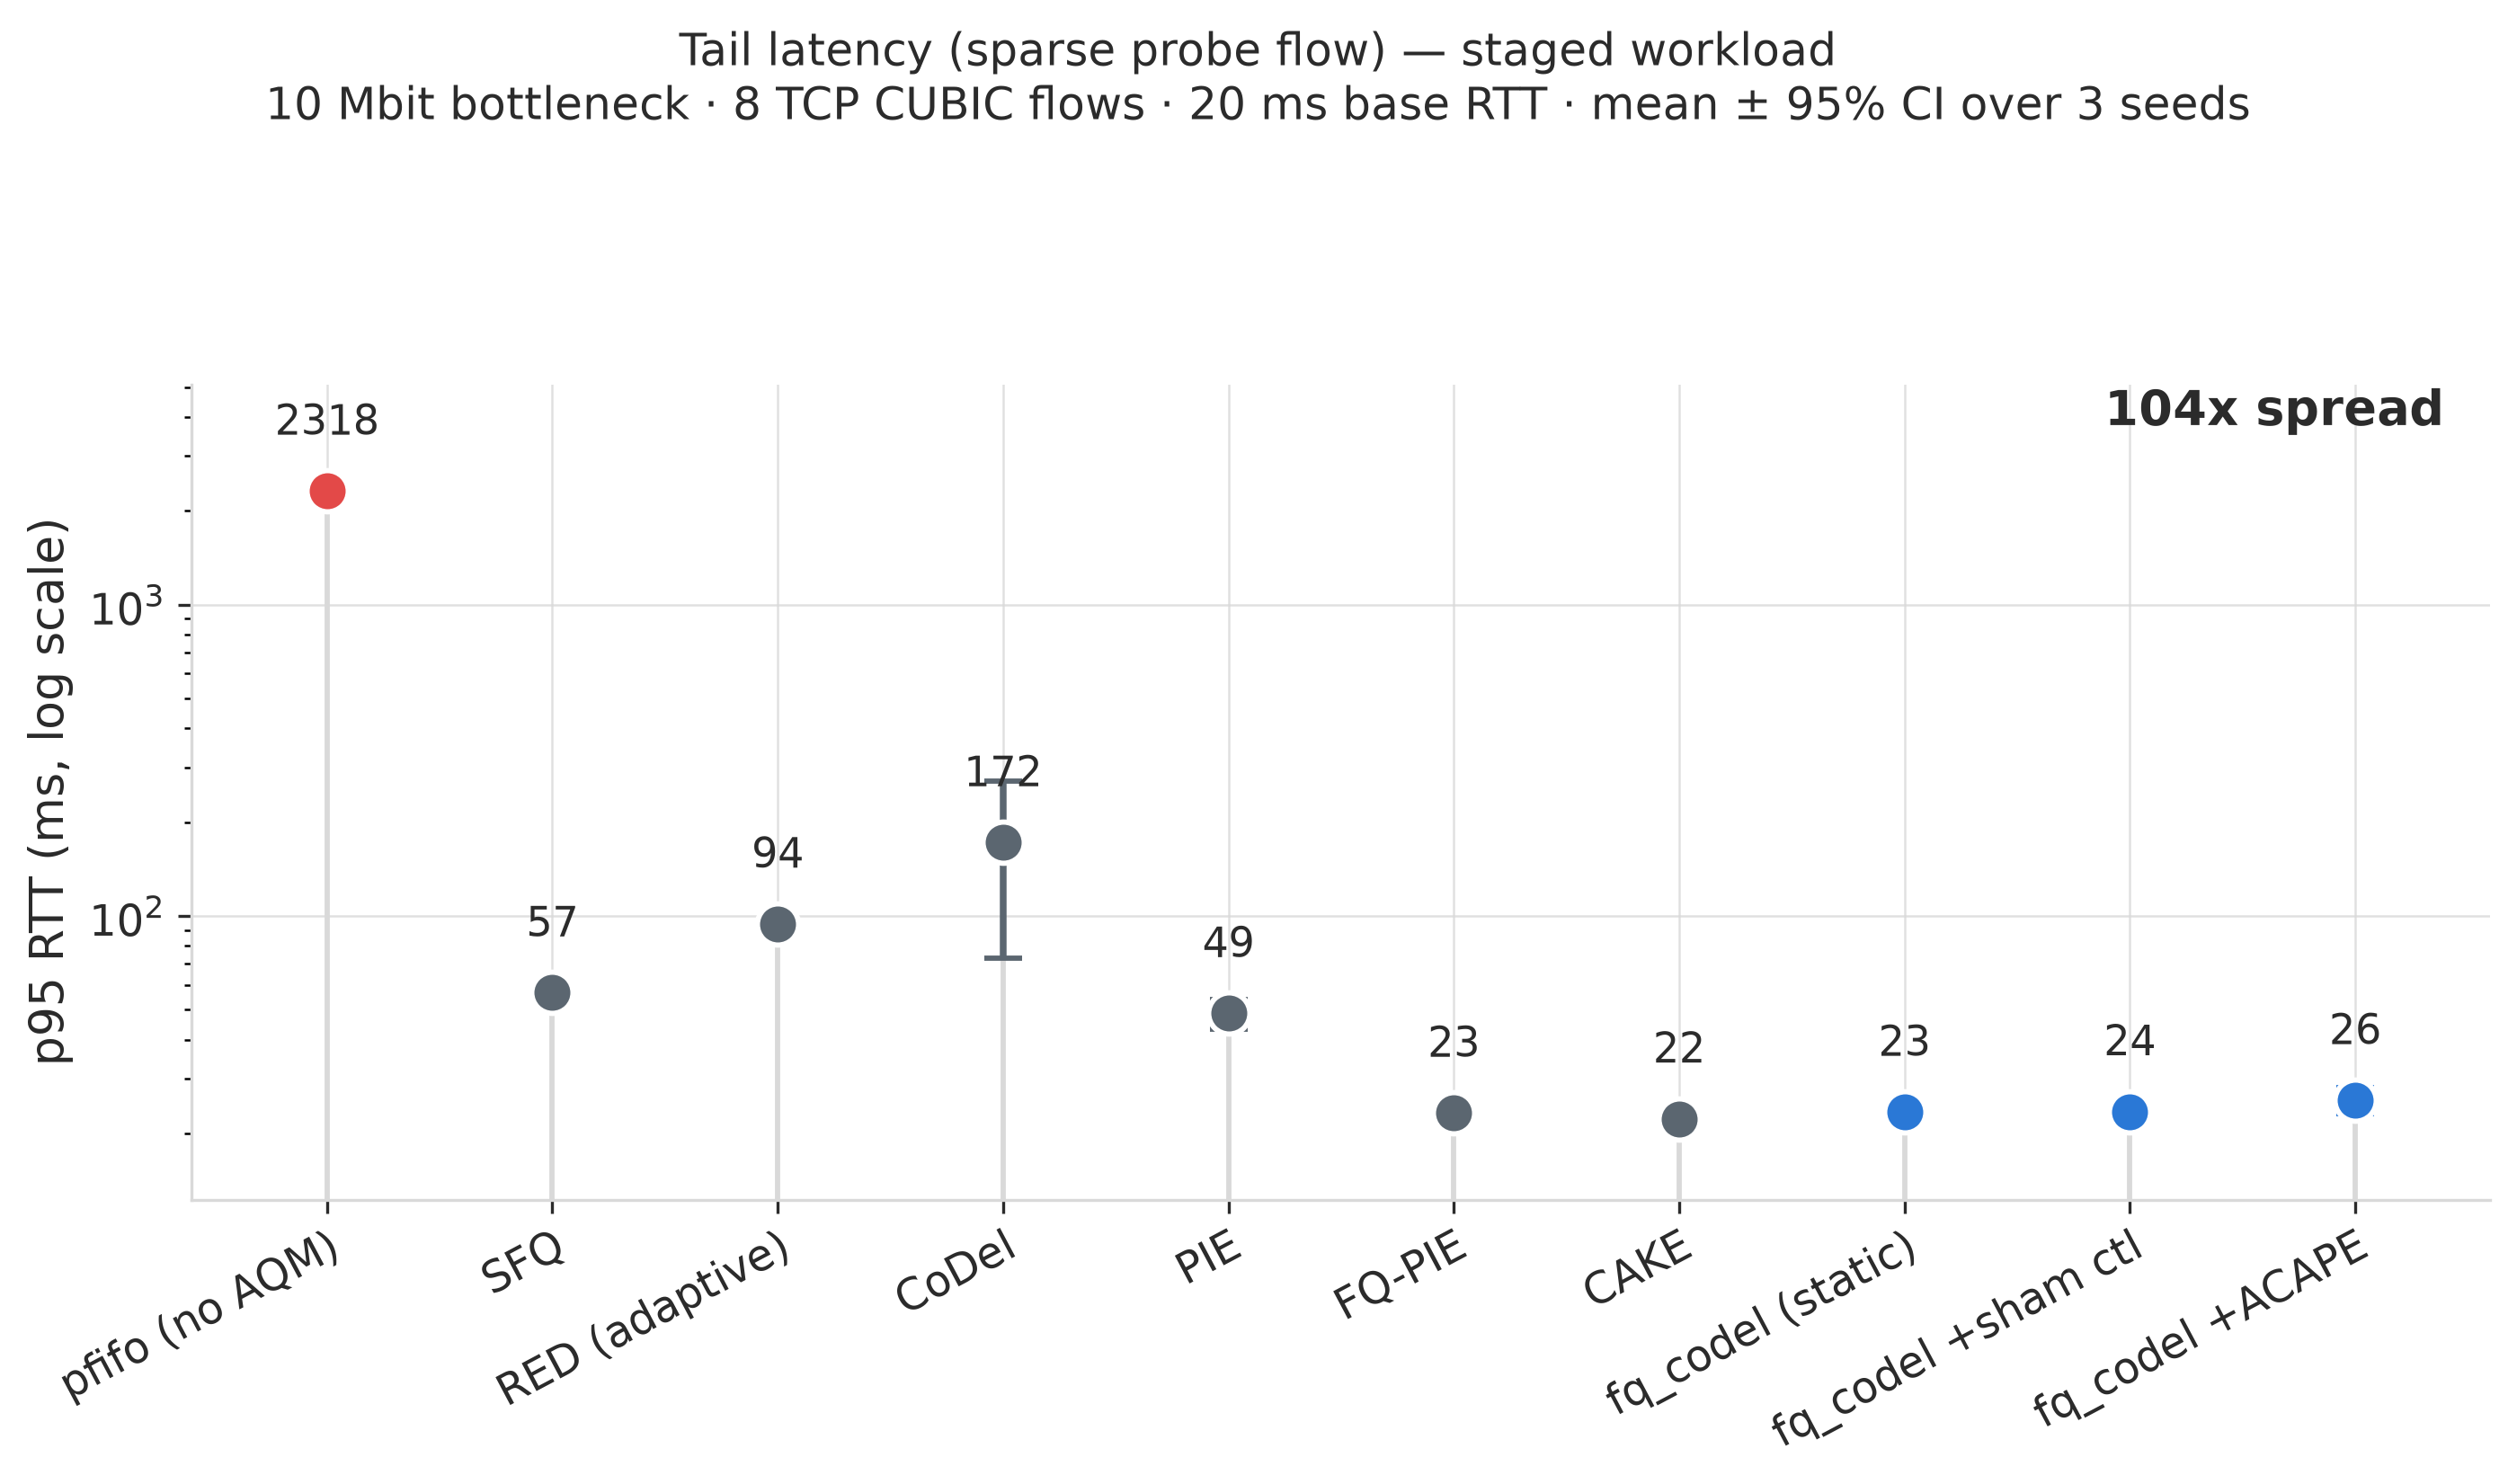
\includegraphics[width=\linewidth,height=0.42\textheight,keepaspectratio]{fig01_latency_tail_staged.png}
\caption{\textbf{FIG 01}: fig01\_latency\_tail\_staged.png. Tail latency (p95 RTT, sparse probe flow) across all systems, log scale (staged workload)}
\end{figure}

\begin{figure}[htbp]
\centering
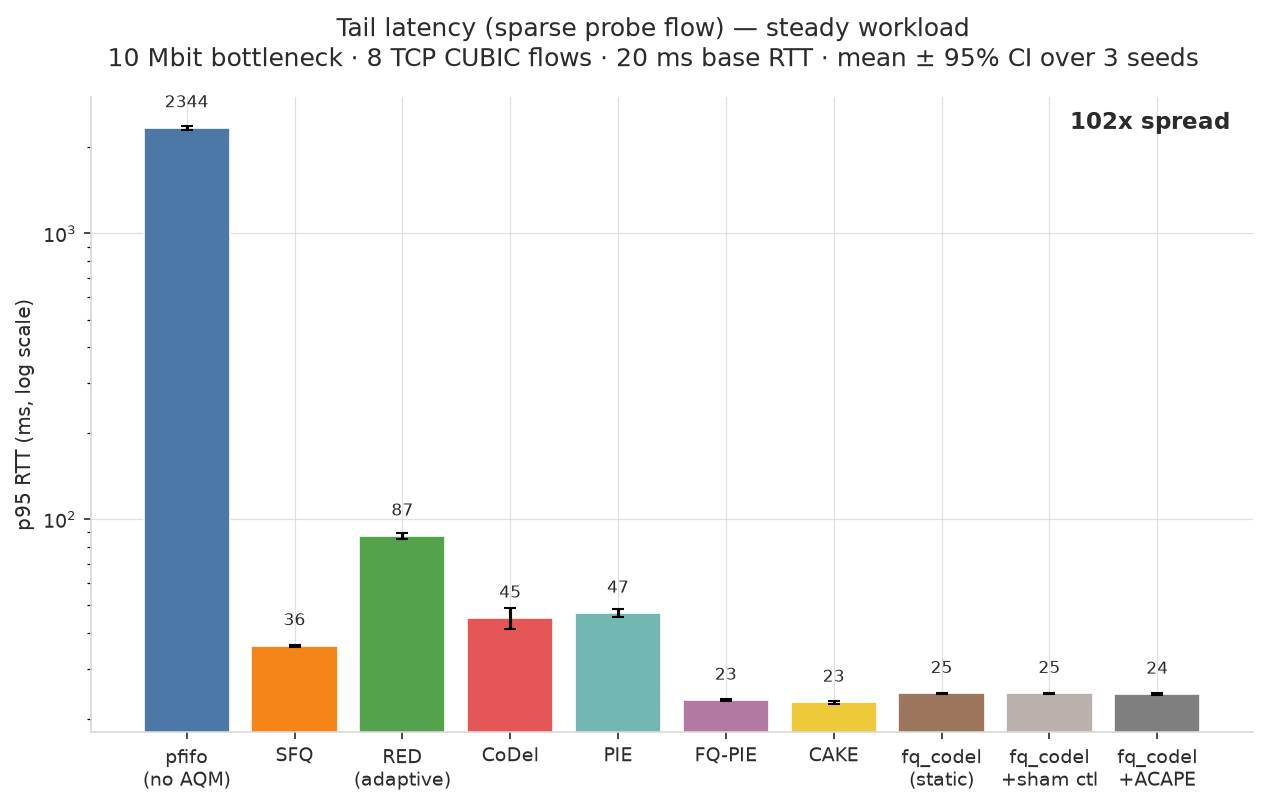
\includegraphics[width=\linewidth,height=0.42\textheight,keepaspectratio]{fig01_latency_tail_steady.png}
\caption{\textbf{FIG 02}: fig01\_latency\_tail\_steady.png. Tail latency (p95 RTT, sparse probe flow) across all systems, log scale (steady workload)}
\end{figure}

\begin{figure}[htbp]
\centering
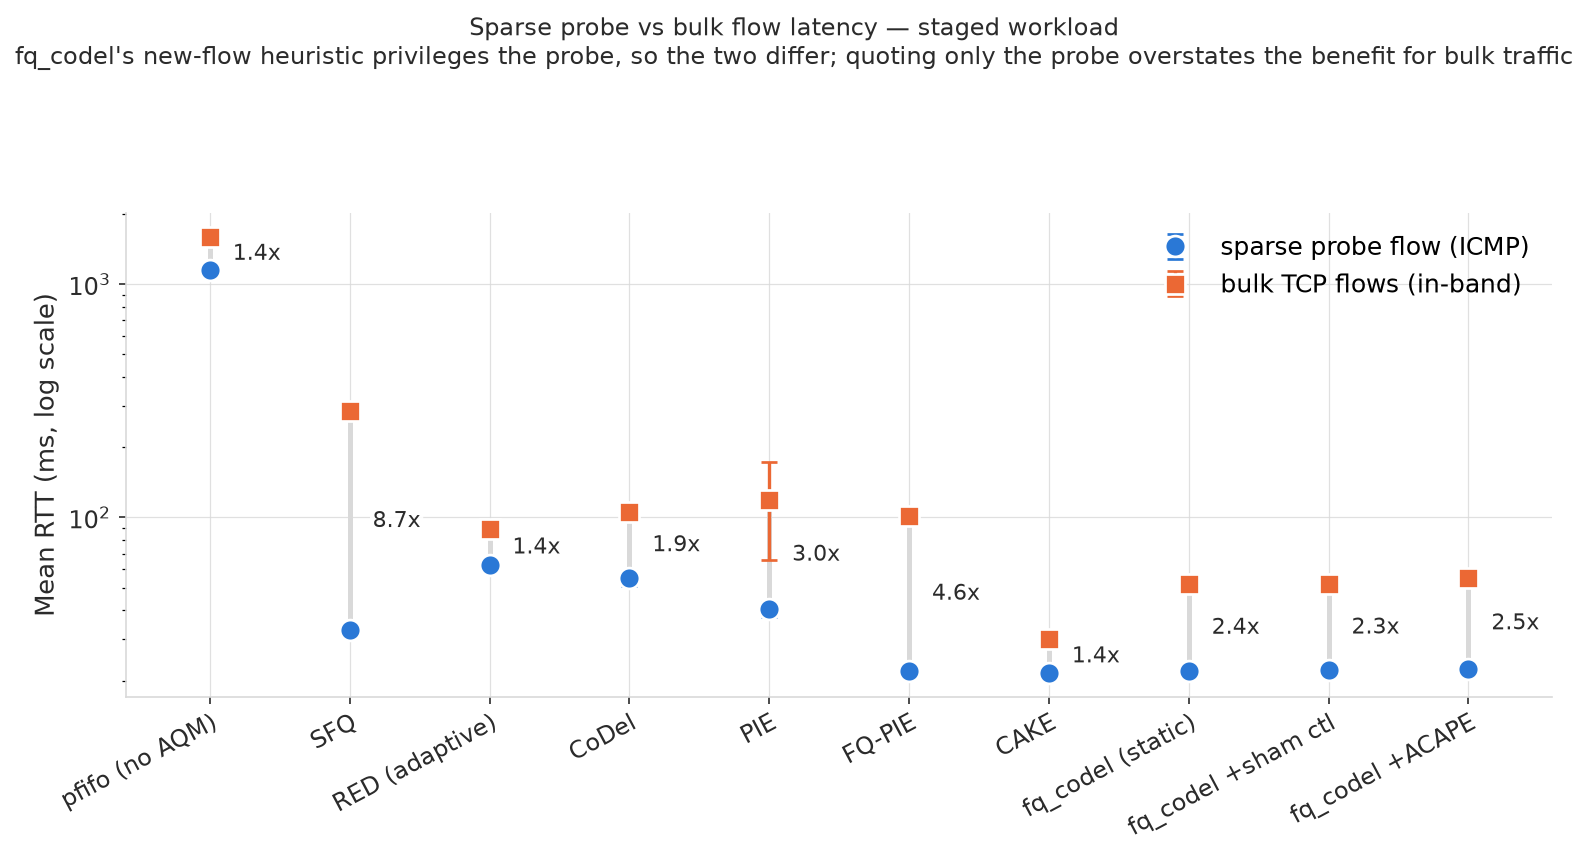
\includegraphics[width=\linewidth,height=0.42\textheight,keepaspectratio]{fig02_latency_sparse_vs_bulk_staged.png}
\caption{\textbf{FIG 03}: fig02\_latency\_sparse\_vs\_bulk\_staged.png. Sparse probe flow vs bulk TCP flow RTT ,  why the two differ (staged workload)}
\end{figure}

\begin{figure}[htbp]
\centering
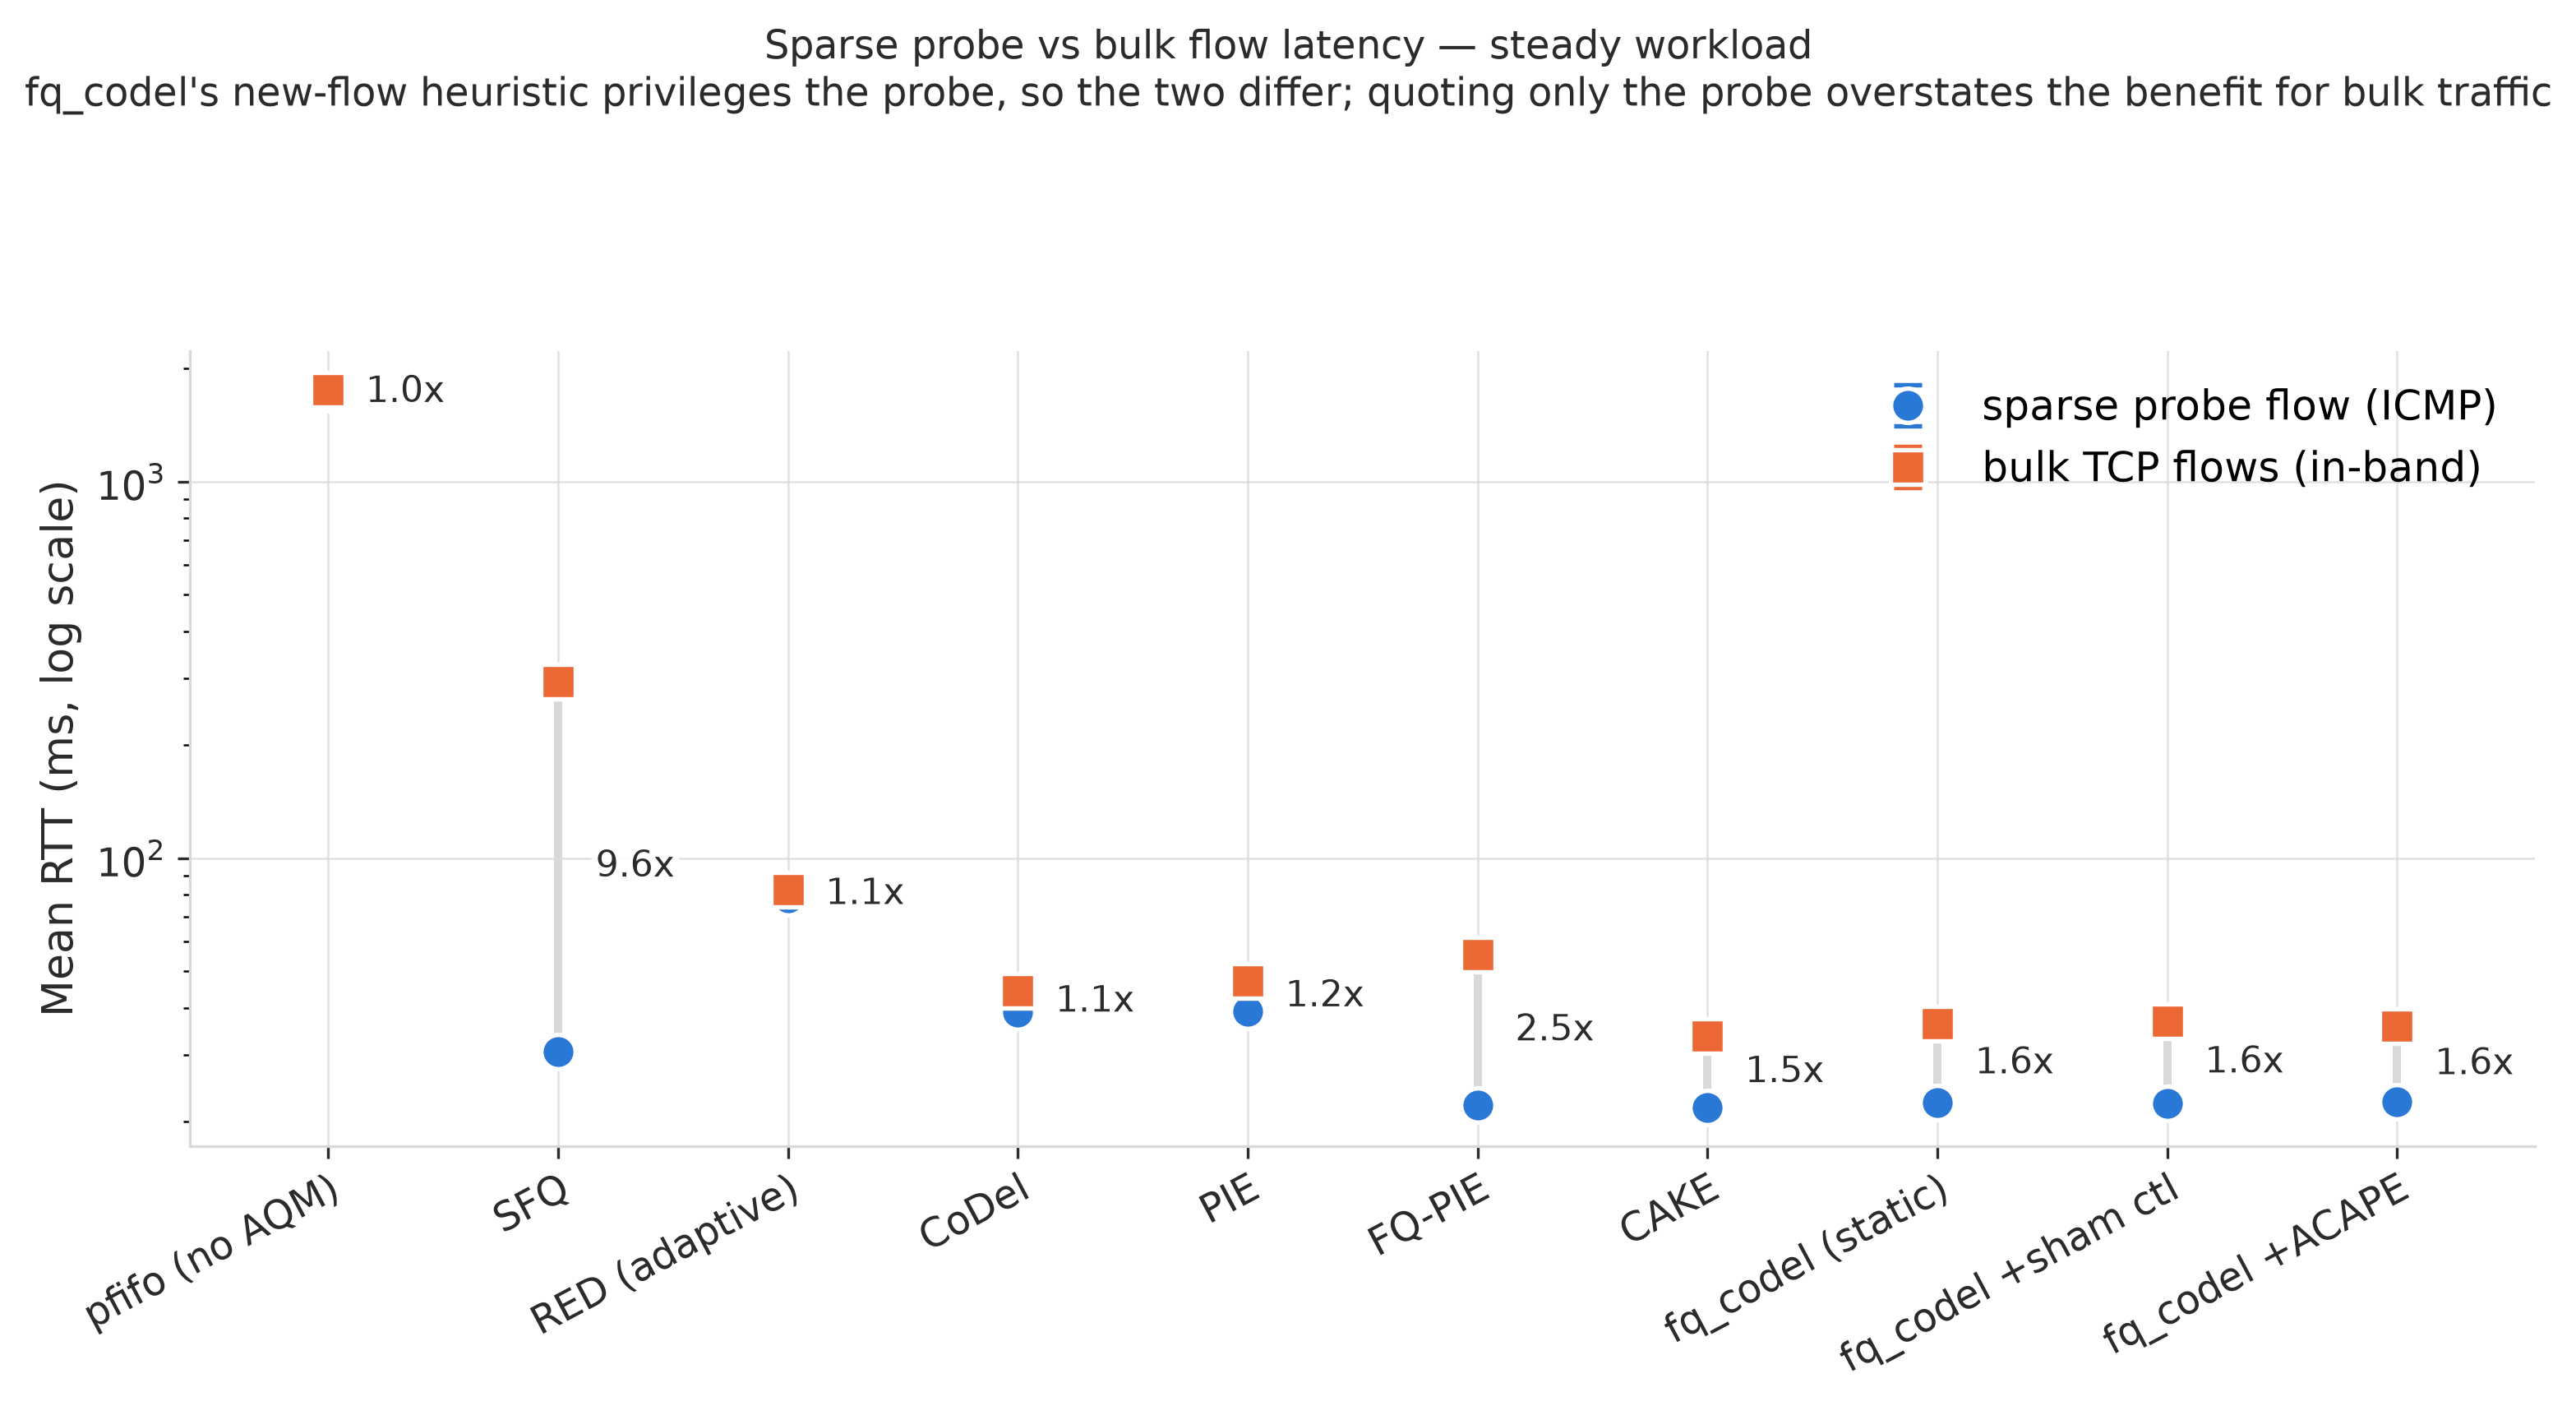
\includegraphics[width=\linewidth,height=0.42\textheight,keepaspectratio]{fig02_latency_sparse_vs_bulk_steady.png}
\caption{\textbf{FIG 04}: fig02\_latency\_sparse\_vs\_bulk\_steady.png. Sparse probe flow vs bulk TCP flow RTT ,  why the two differ (steady workload)}
\end{figure}

\begin{figure}[htbp]
\centering
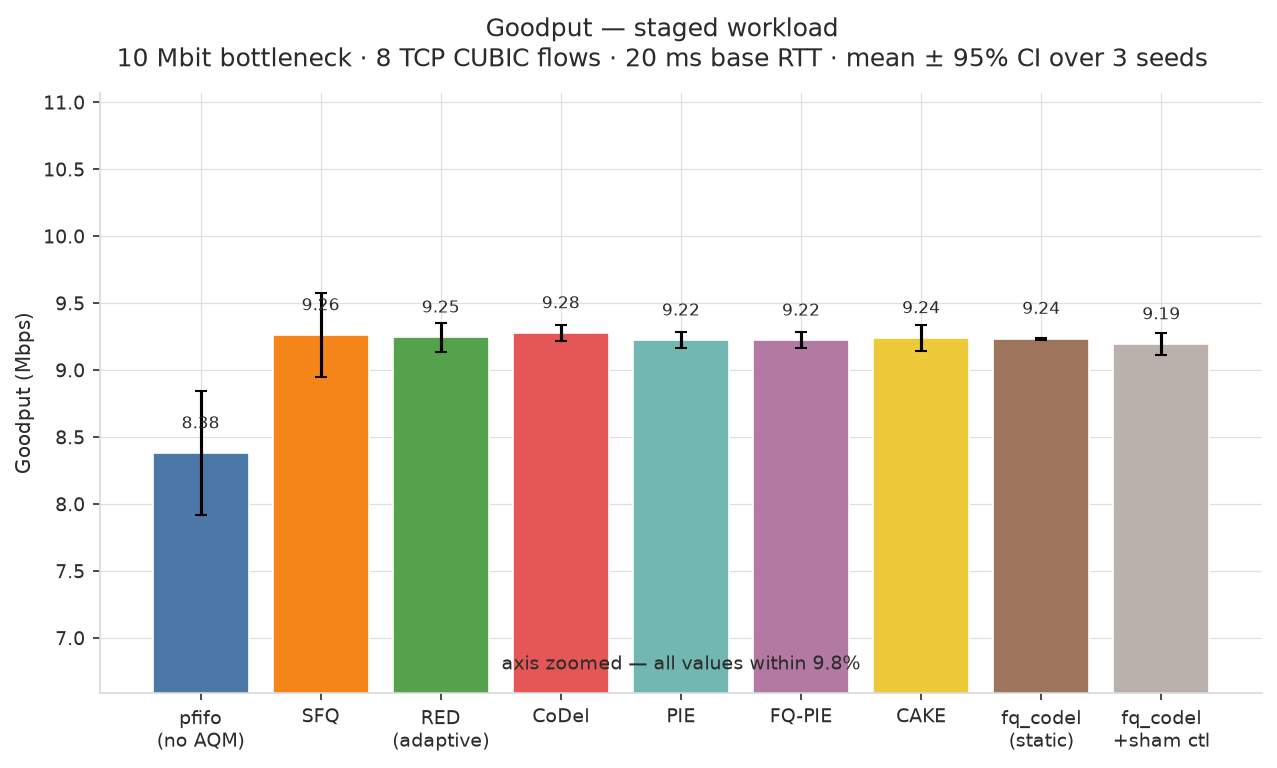
\includegraphics[width=\linewidth,height=0.42\textheight,keepaspectratio]{fig03_throughput_staged.png}
\caption{\textbf{FIG 05}: fig03\_throughput\_staged.png. Goodput (from iperf3 sum\_received), axis zoomed to show it is flat (staged workload)}
\end{figure}

\begin{figure}[htbp]
\centering
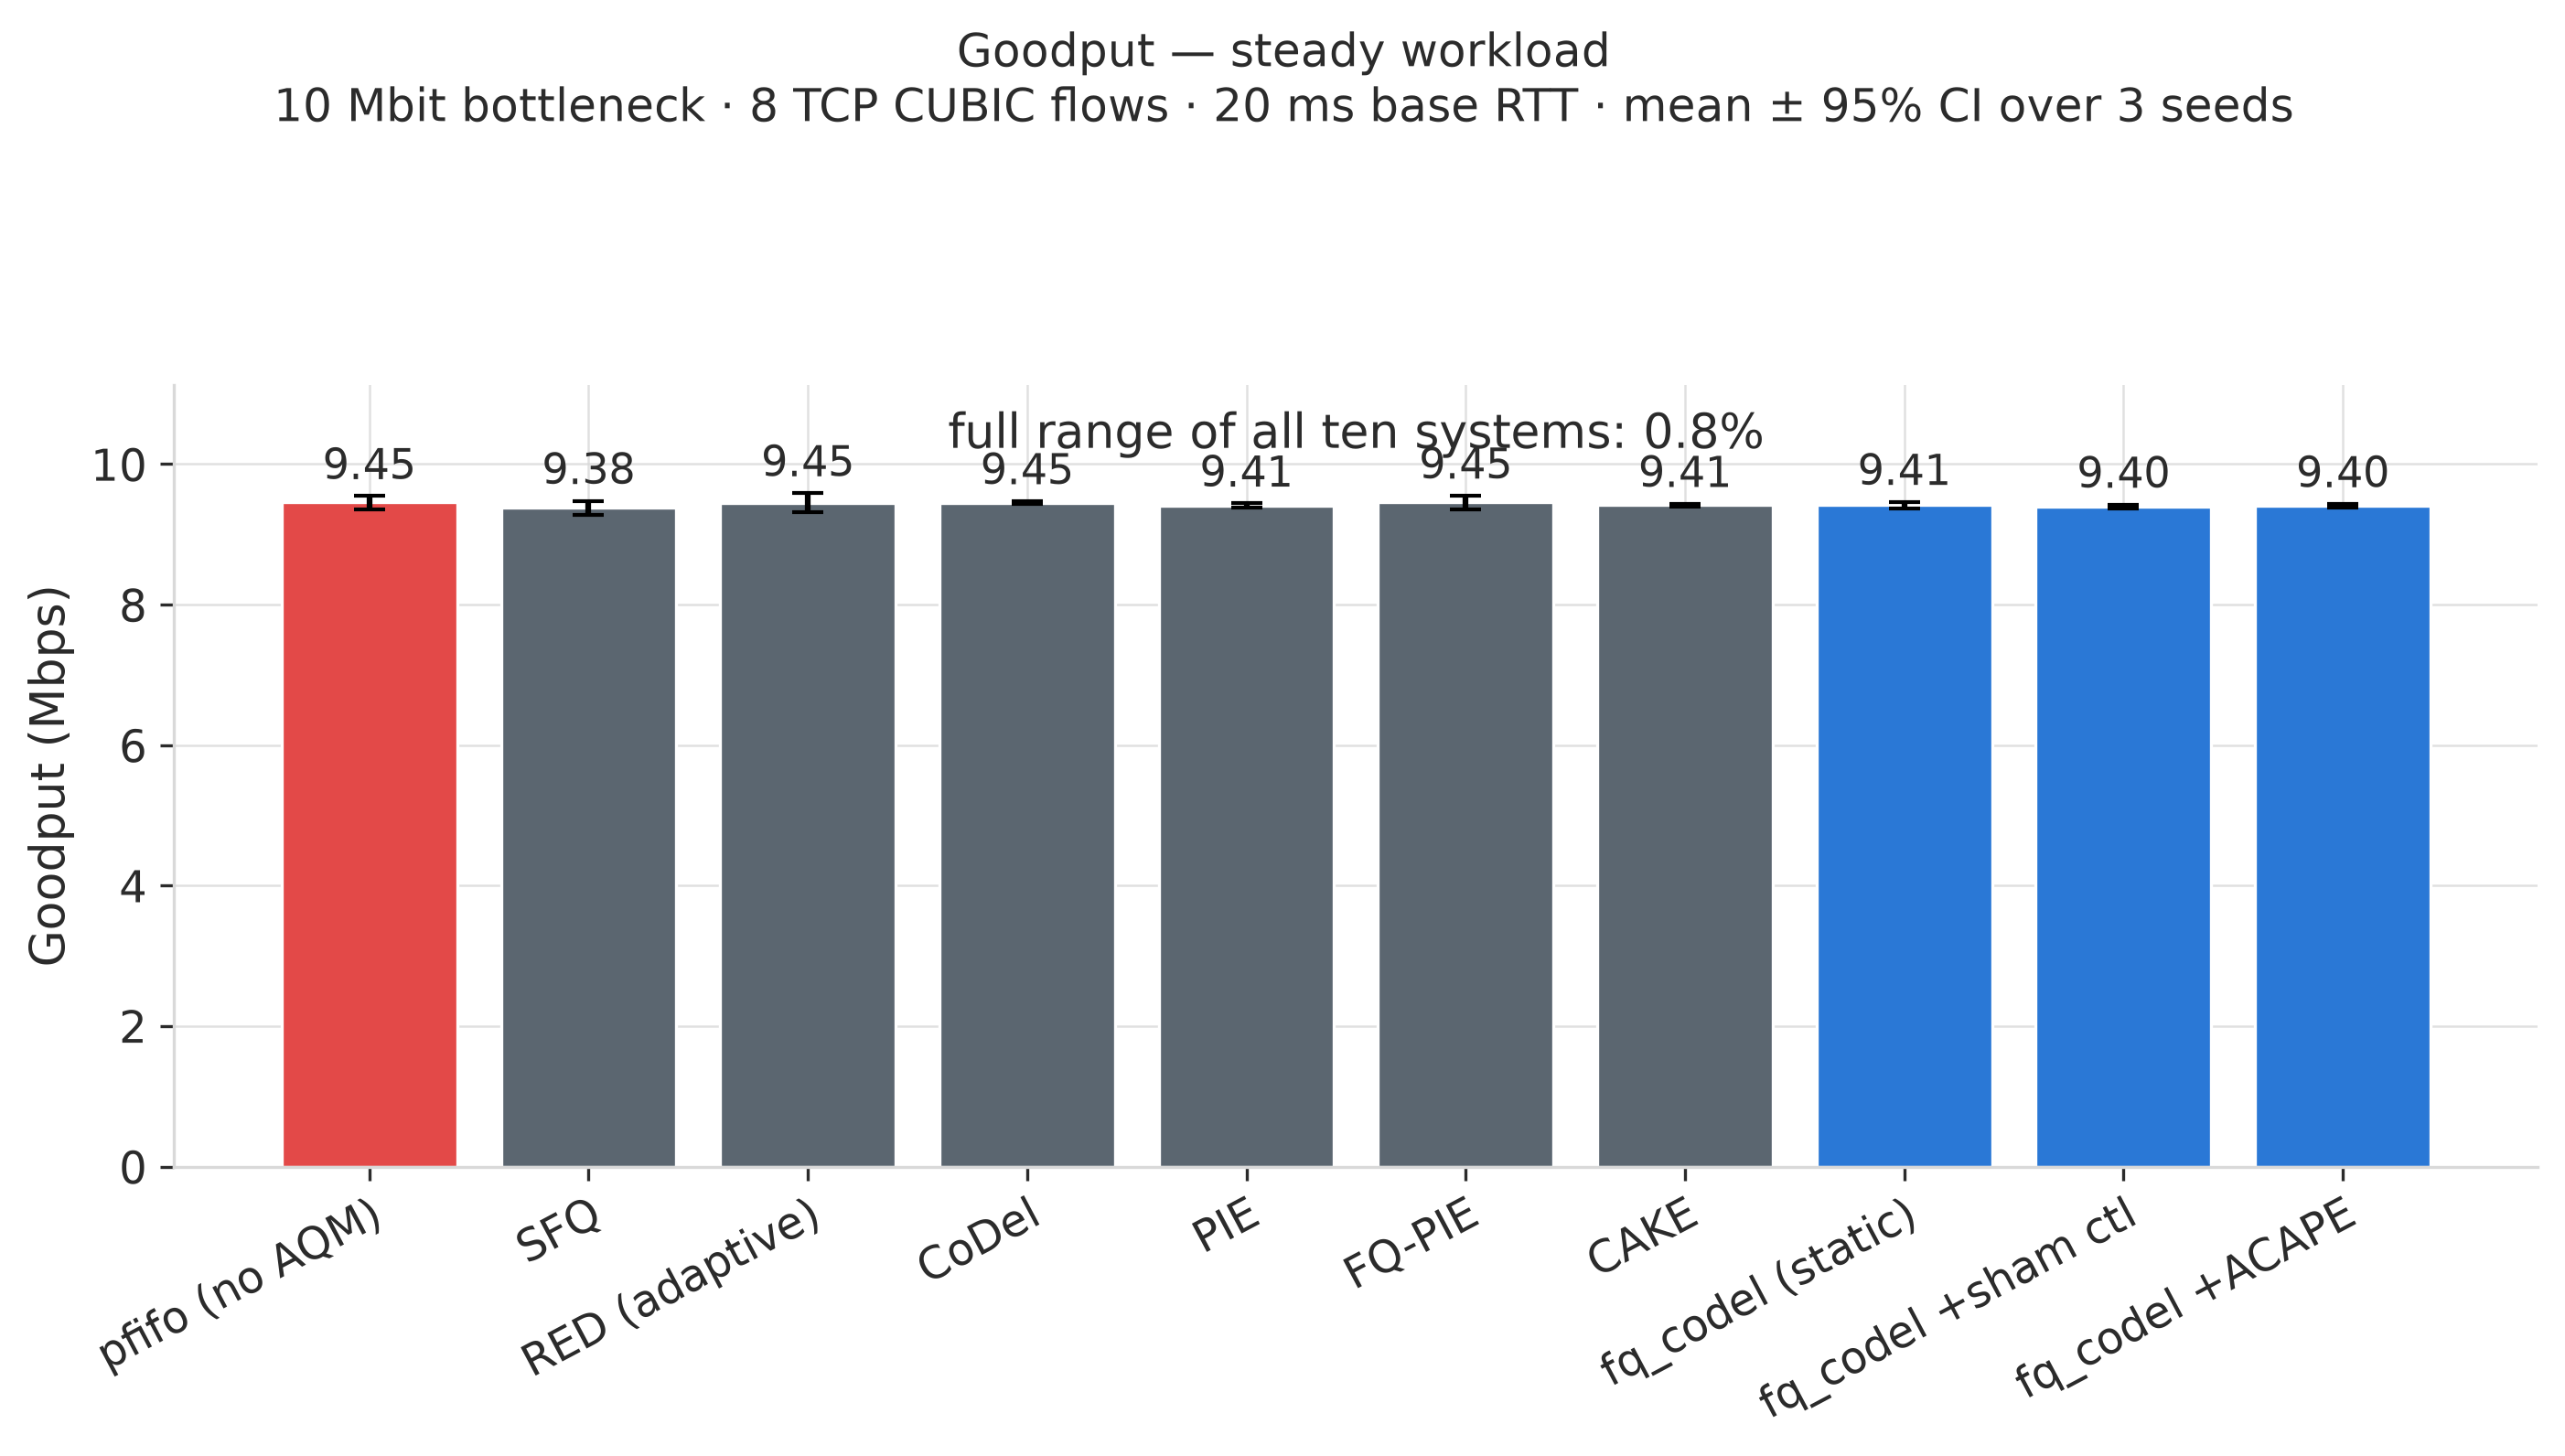
\includegraphics[width=\linewidth,height=0.42\textheight,keepaspectratio]{fig03_throughput_steady.png}
\caption{\textbf{FIG 06}: fig03\_throughput\_steady.png. Goodput (from iperf3 sum\_received), axis zoomed to show it is flat (steady workload)}
\end{figure}

\begin{figure}[htbp]
\centering
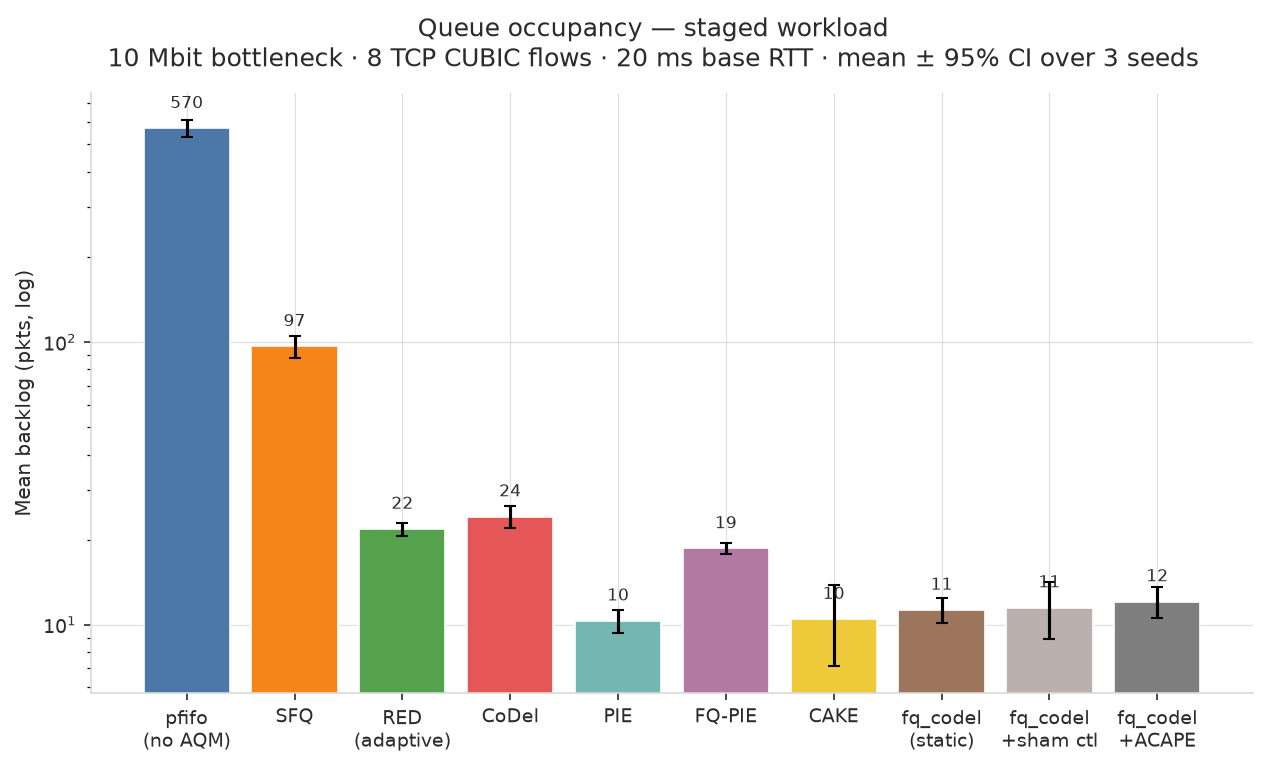
\includegraphics[width=\linewidth,height=0.42\textheight,keepaspectratio]{fig04_backlog_staged.png}
\caption{\textbf{FIG 07}: fig04\_backlog\_staged.png. Mean queue occupancy, log scale (staged workload)}
\end{figure}

\begin{figure}[htbp]
\centering
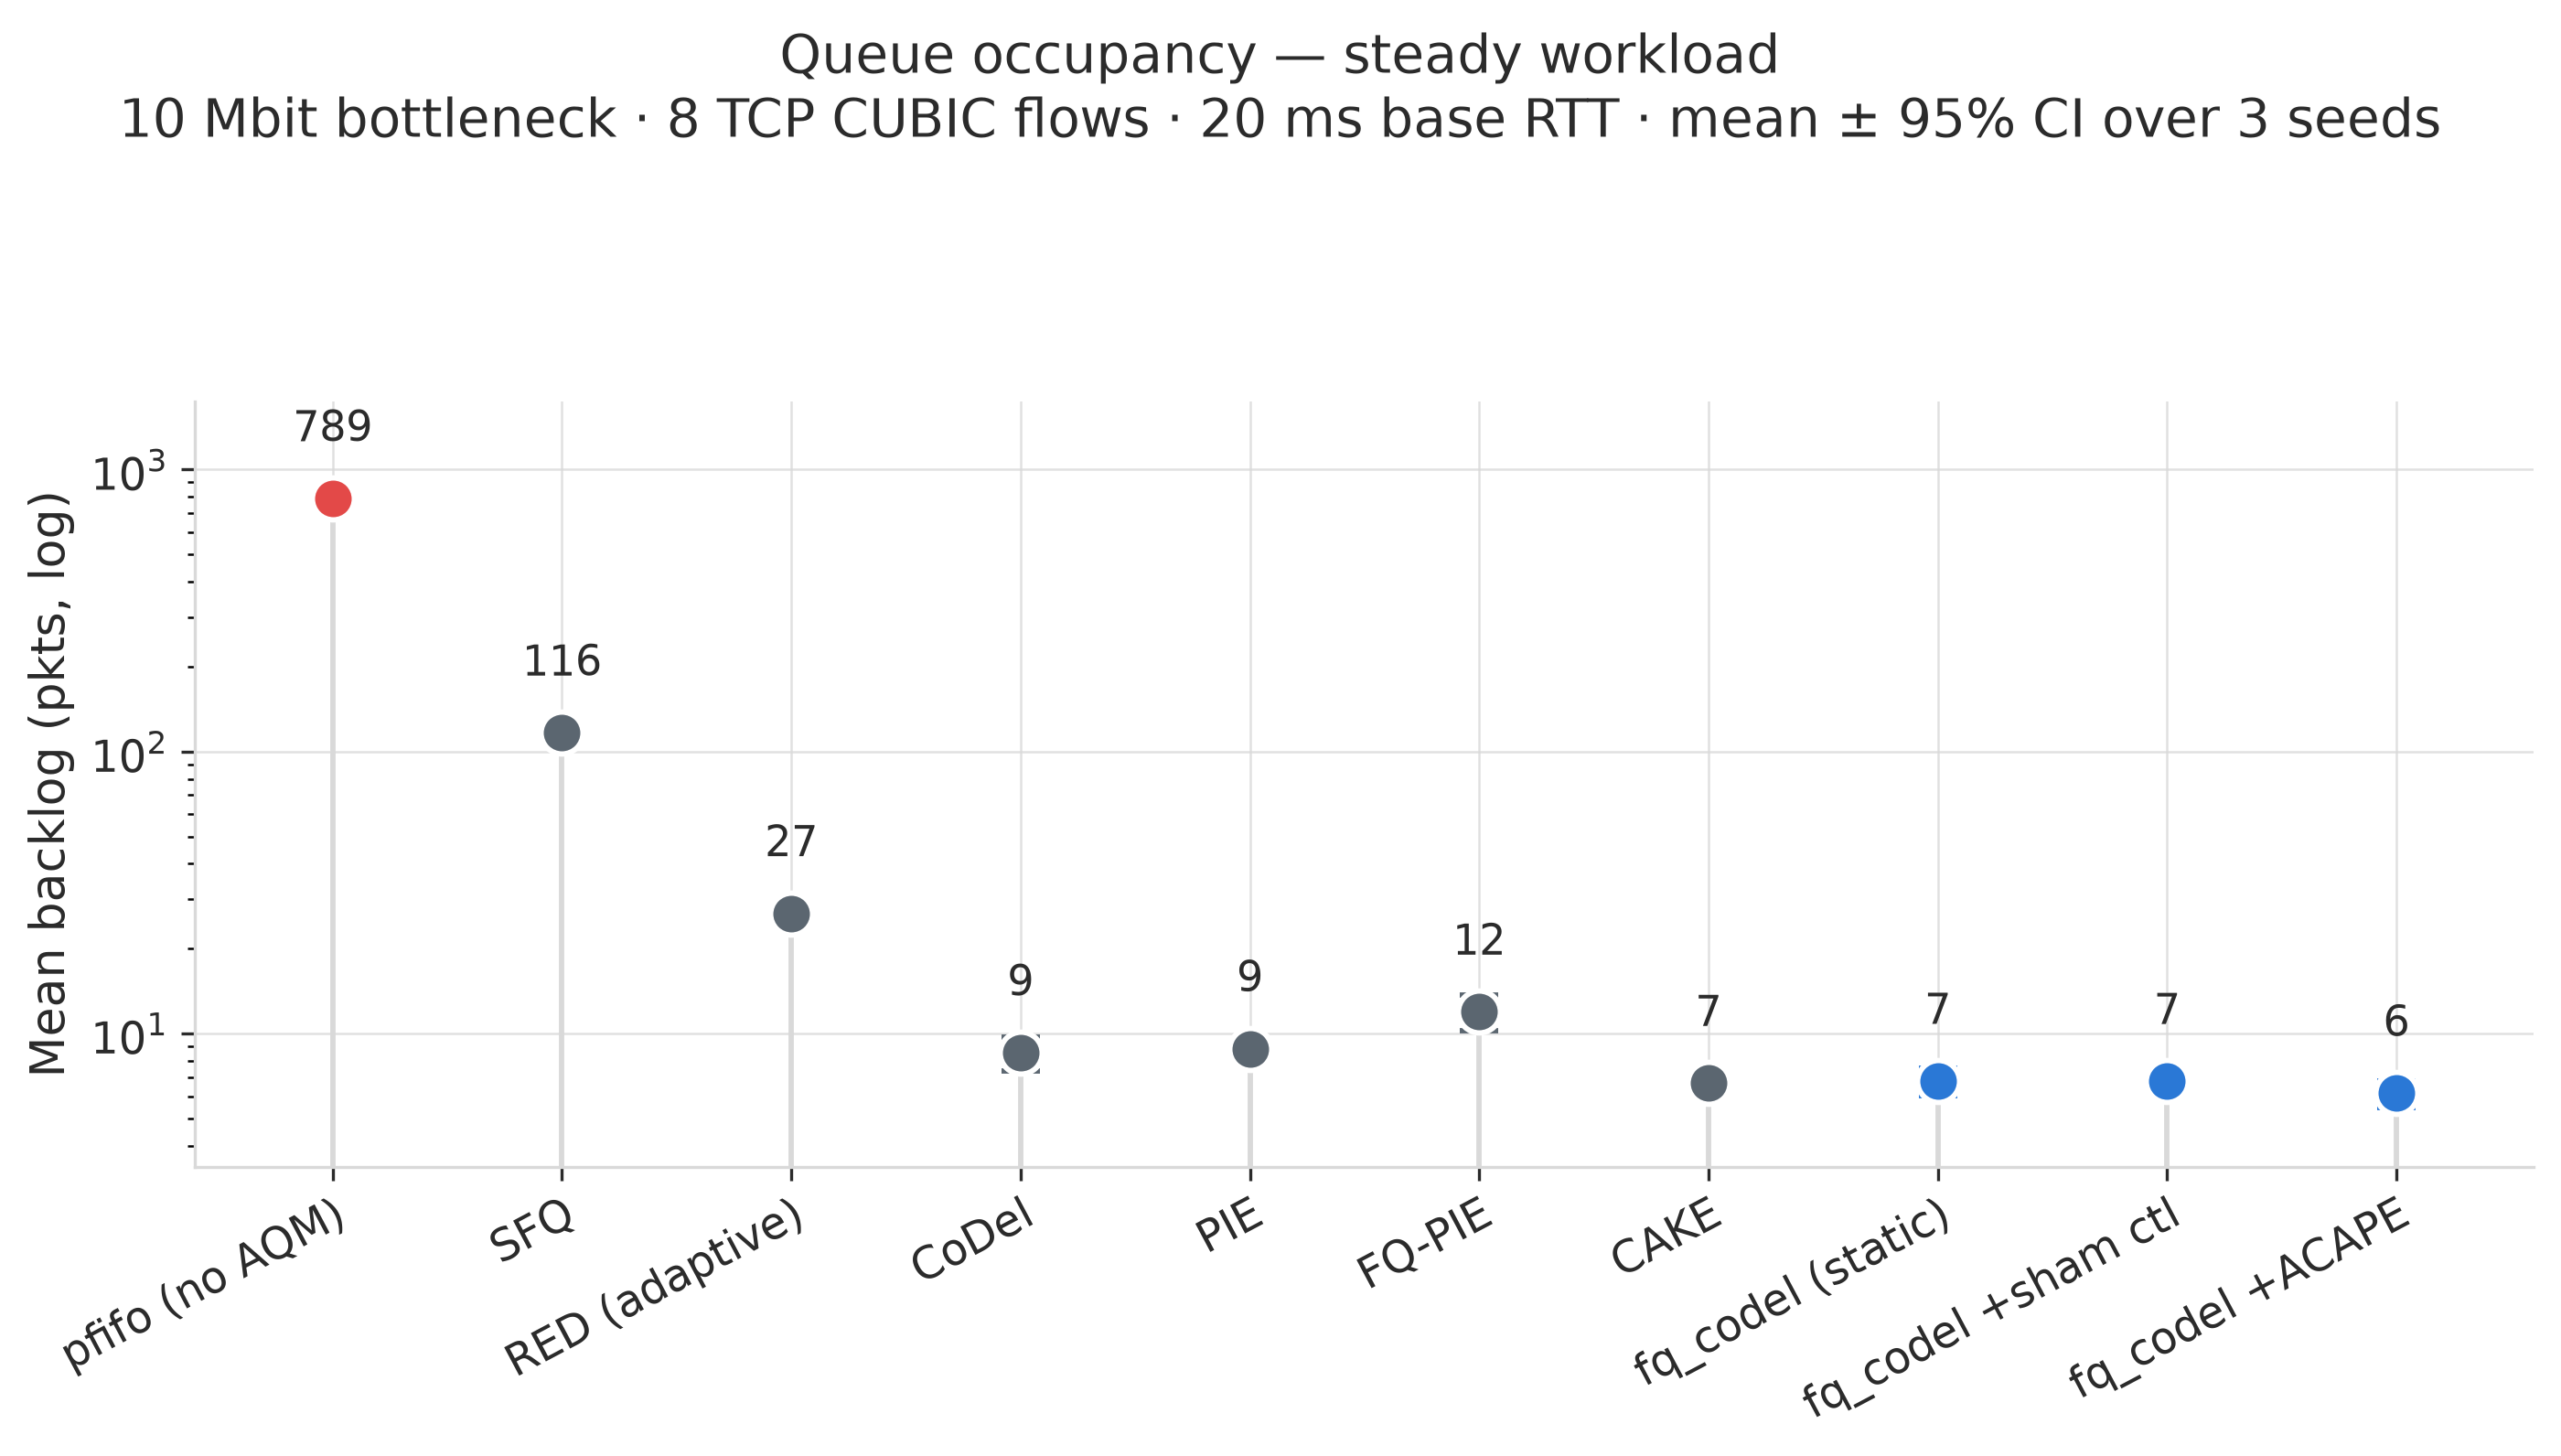
\includegraphics[width=\linewidth,height=0.42\textheight,keepaspectratio]{fig04_backlog_steady.png}
\caption{\textbf{FIG 08}: fig04\_backlog\_steady.png. Mean queue occupancy, log scale (steady workload)}
\end{figure}

\begin{figure}[htbp]
\centering
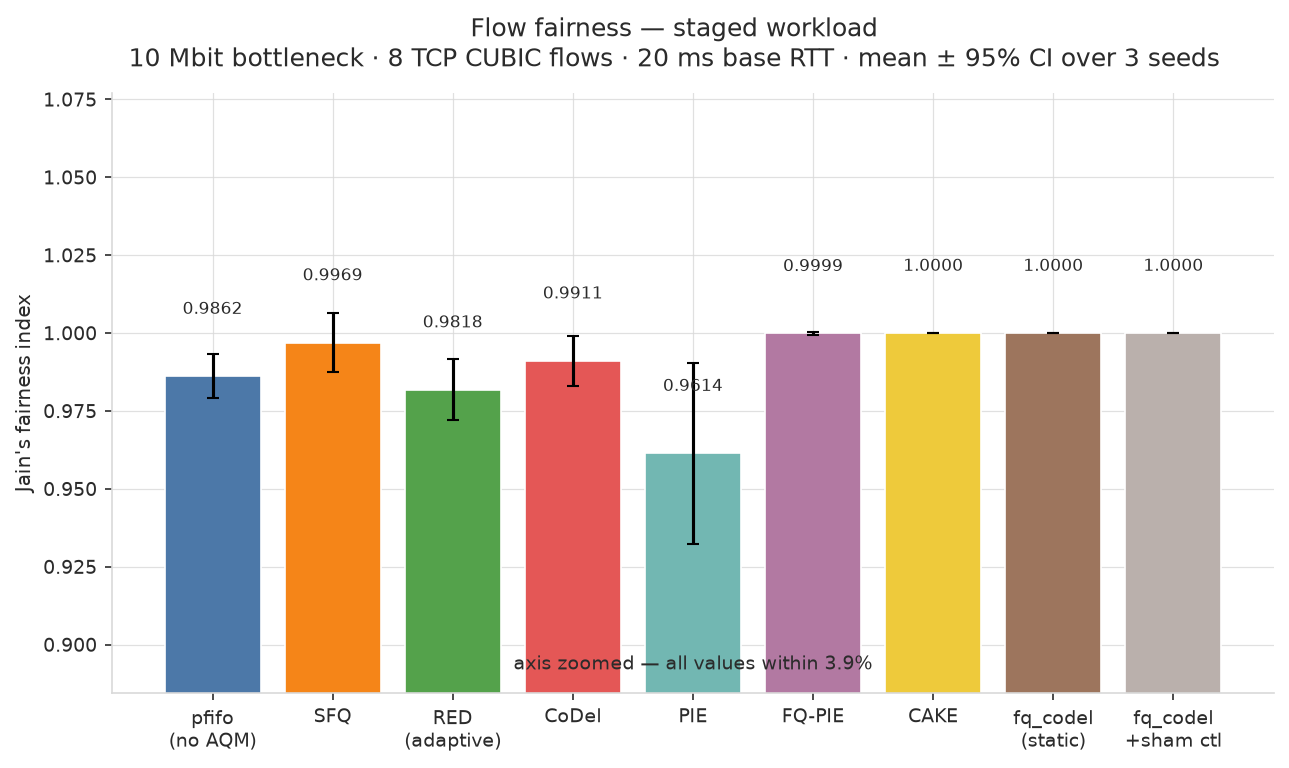
\includegraphics[width=\linewidth,height=0.42\textheight,keepaspectratio]{fig05_fairness_staged.png}
\caption{\textbf{FIG 09}: fig05\_fairness\_staged.png. Jain's fairness index, axis zoomed (staged workload)}
\end{figure}

\begin{figure}[htbp]
\centering
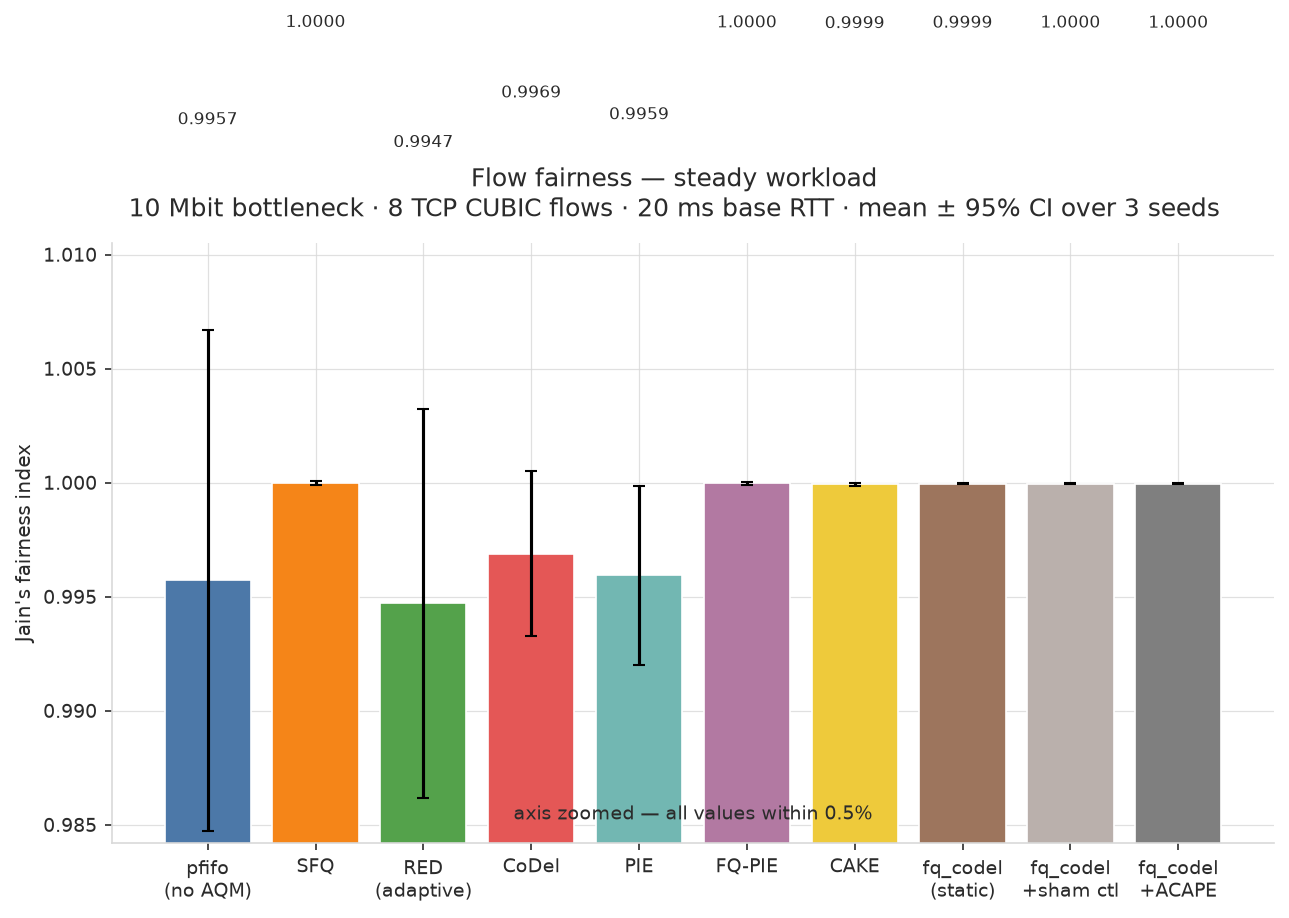
\includegraphics[width=\linewidth,height=0.42\textheight,keepaspectratio]{fig05_fairness_steady.png}
\caption{\textbf{FIG 10}: fig05\_fairness\_steady.png. Jain's fairness index, axis zoomed (steady workload)}
\end{figure}

\begin{figure}[htbp]
\centering
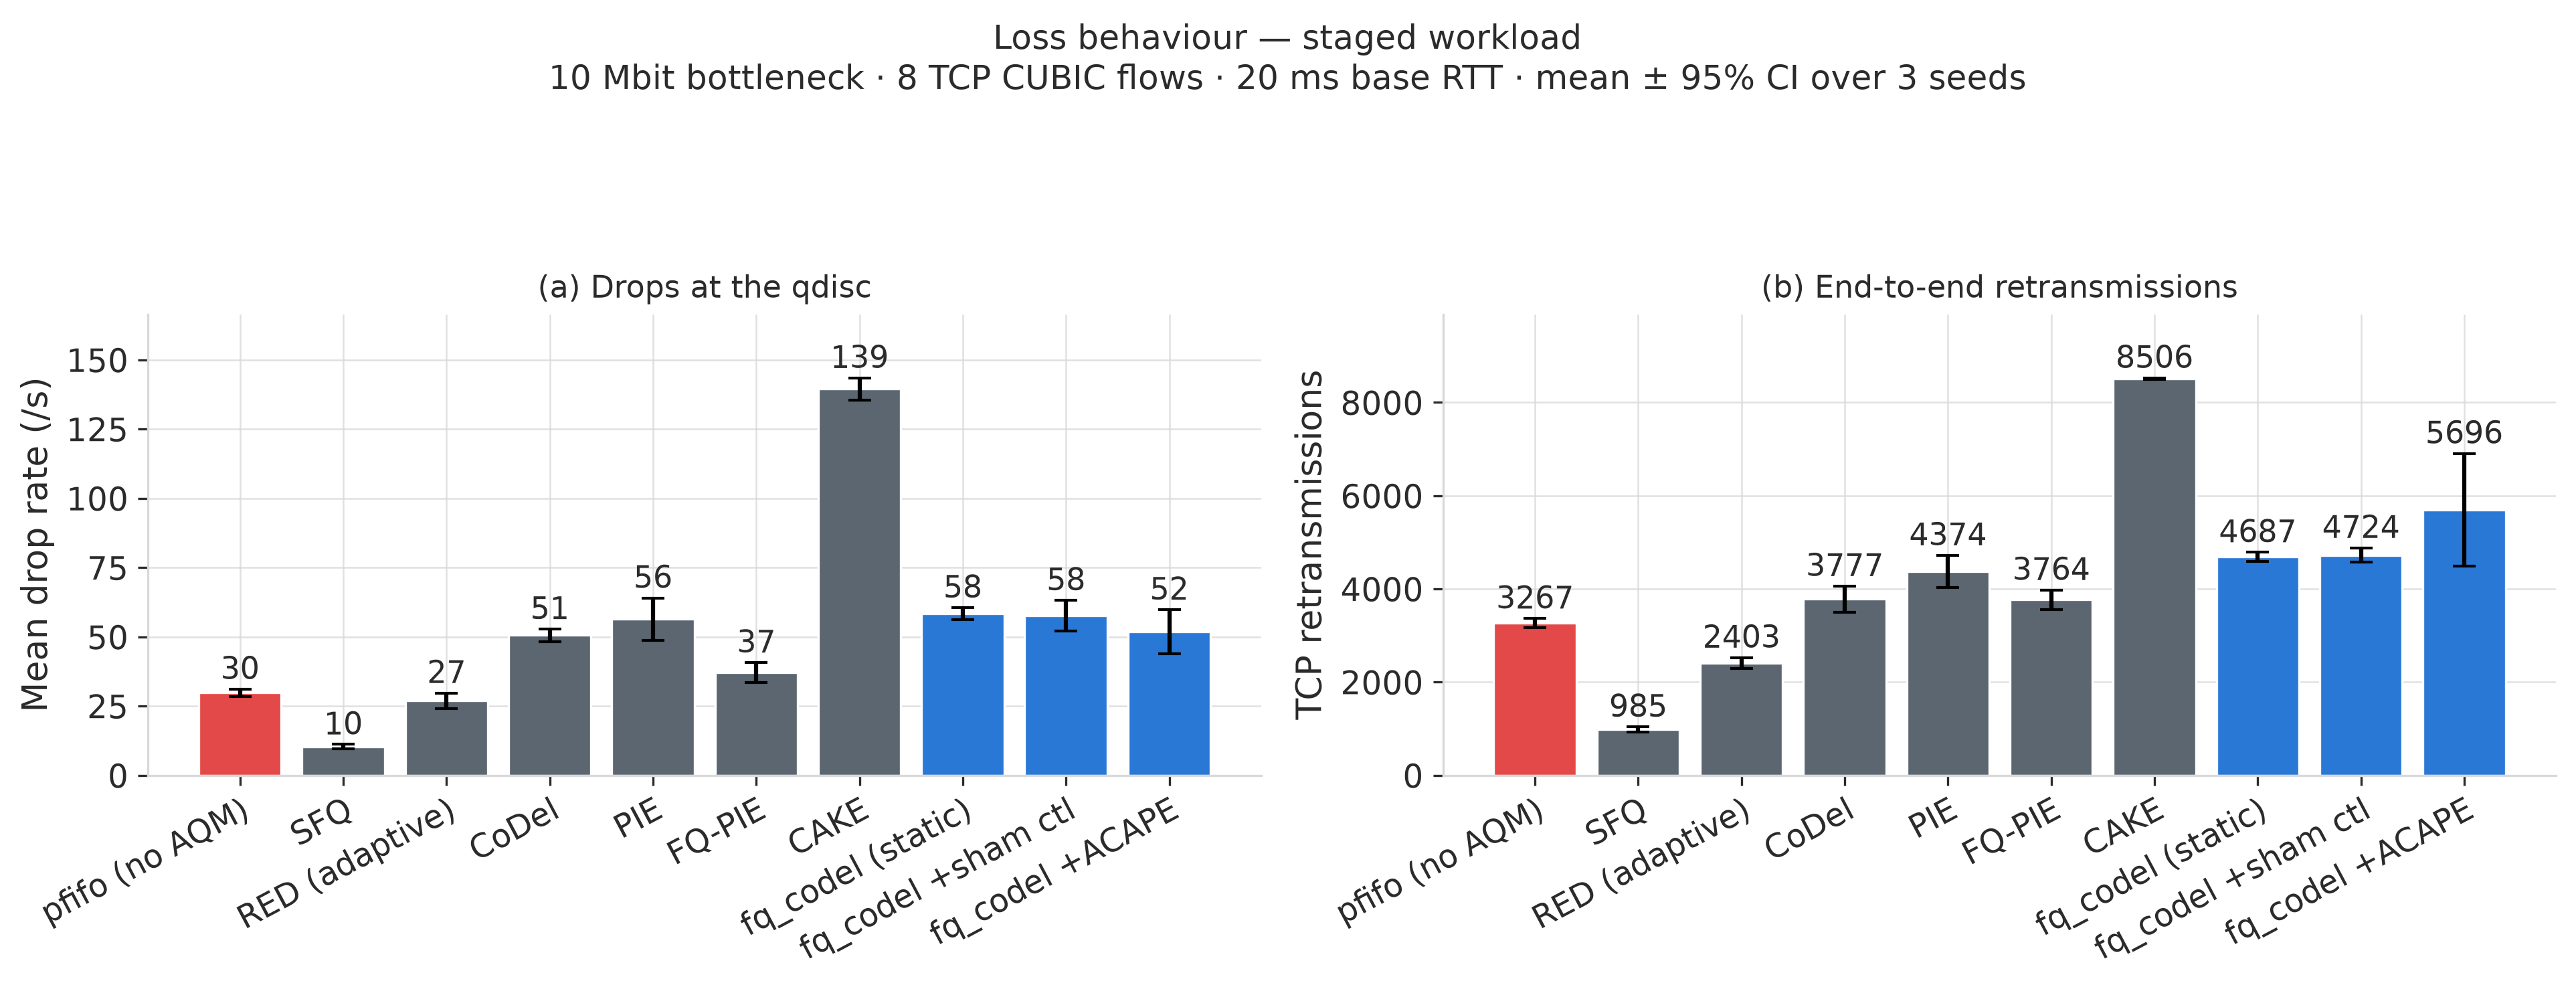
\includegraphics[width=\linewidth,height=0.42\textheight,keepaspectratio]{fig06_droprate_staged.png}
\caption{\textbf{FIG 11}: fig06\_droprate\_staged.png. AQM drop rate and end-to-end TCP retransmissions (staged workload)}
\end{figure}

\begin{figure}[htbp]
\centering
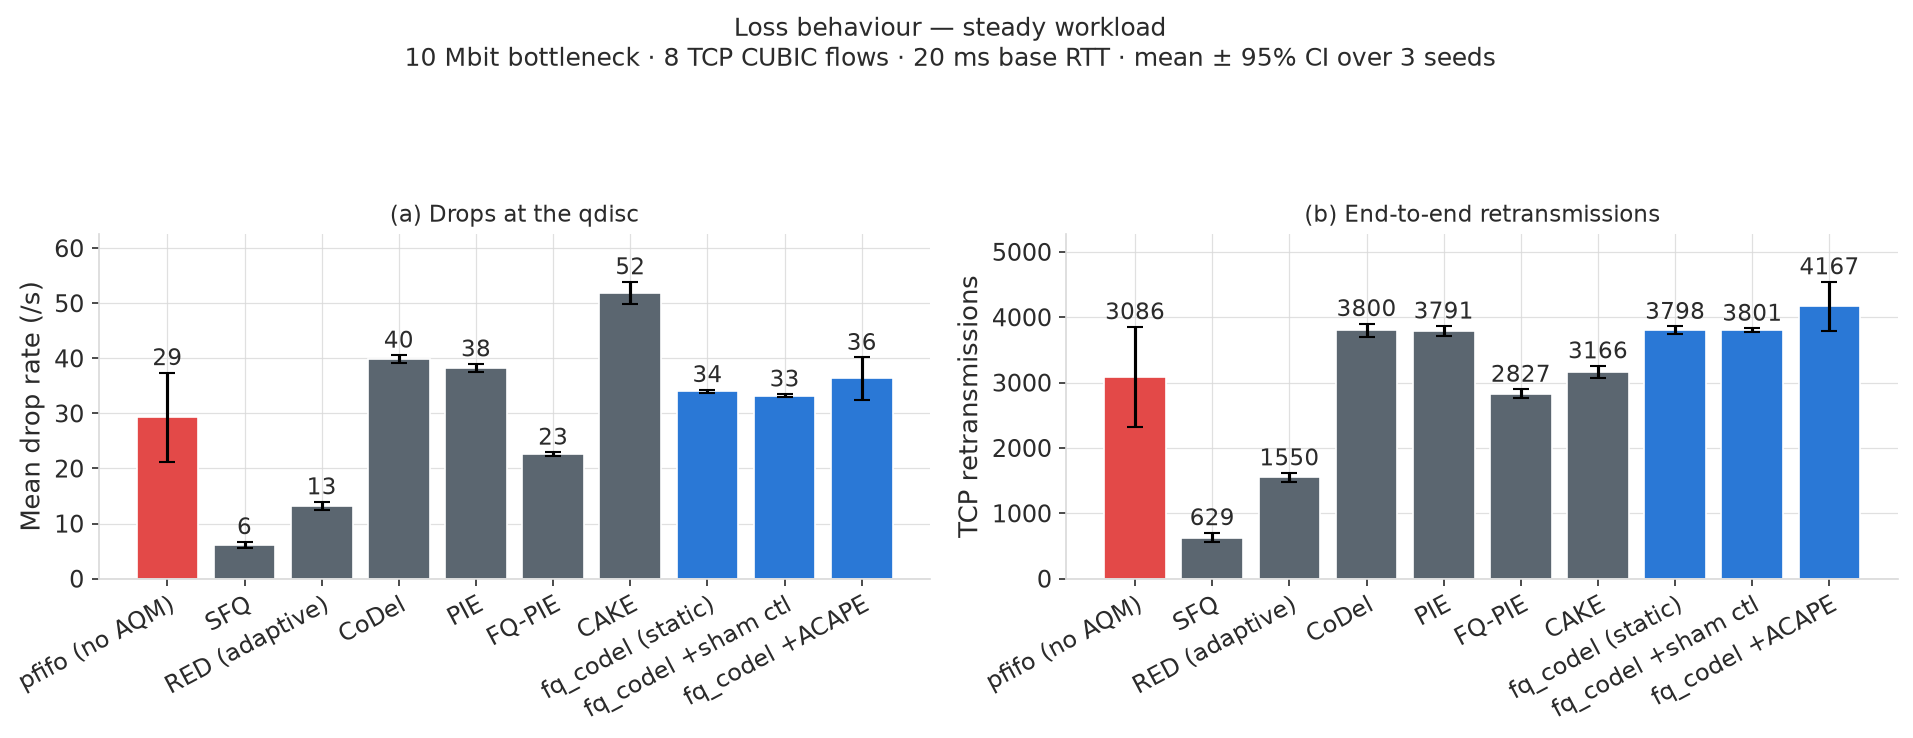
\includegraphics[width=\linewidth,height=0.42\textheight,keepaspectratio]{fig06_droprate_steady.png}
\caption{\textbf{FIG 12}: fig06\_droprate\_steady.png. AQM drop rate and end-to-end TCP retransmissions (steady workload)}
\end{figure}

\begin{figure}[htbp]
\centering
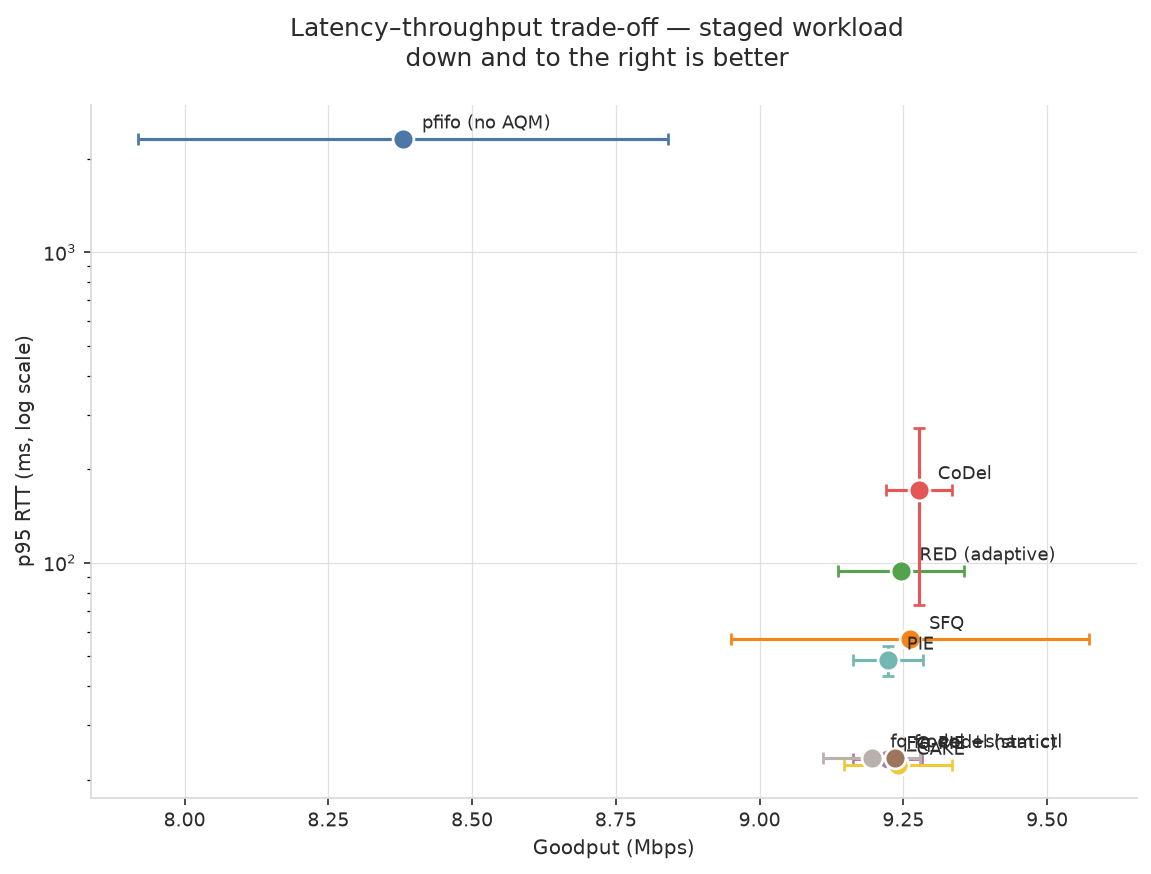
\includegraphics[width=\linewidth,height=0.42\textheight,keepaspectratio]{fig07_tradeoff_staged.png}
\caption{\textbf{FIG 13}: fig07\_tradeoff\_staged.png. Latency vs throughput trade-off (staged workload)}
\end{figure}

\begin{figure}[htbp]
\centering
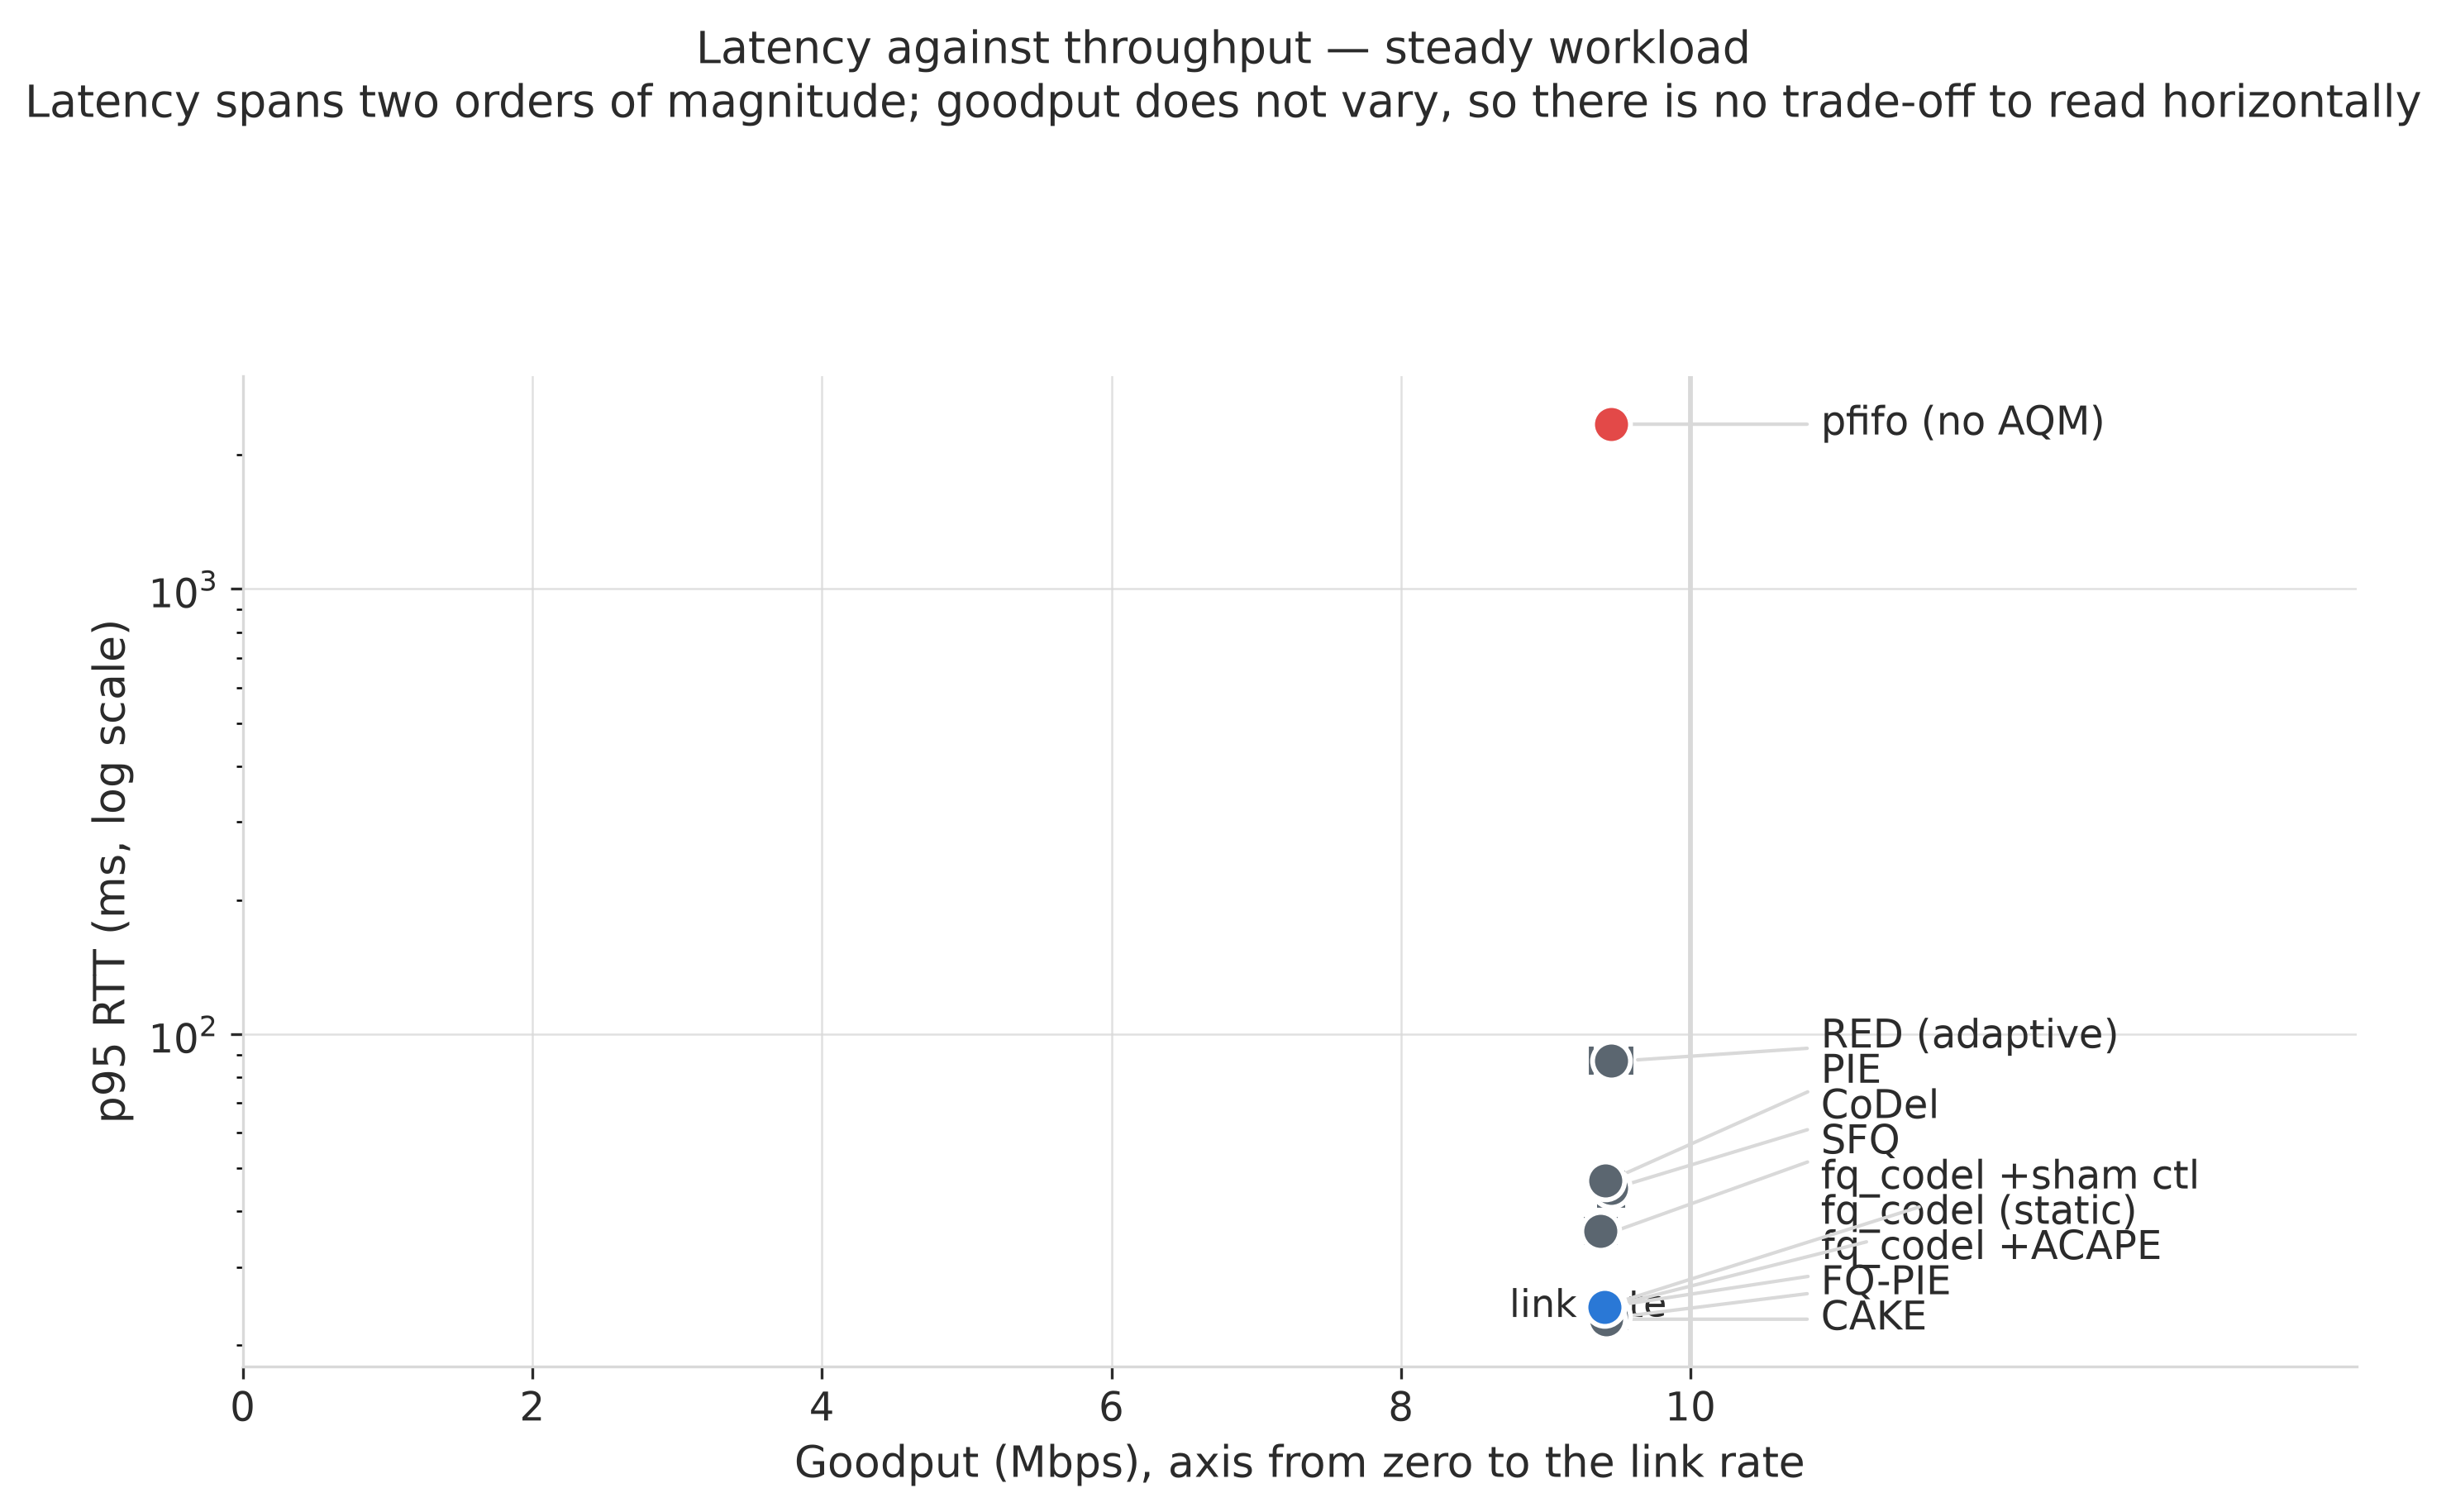
\includegraphics[width=\linewidth,height=0.42\textheight,keepaspectratio]{fig07_tradeoff_steady.png}
\caption{\textbf{FIG 14}: fig07\_tradeoff\_steady.png. Latency vs throughput trade-off (steady workload)}
\end{figure}

\begin{figure}[htbp]
\centering
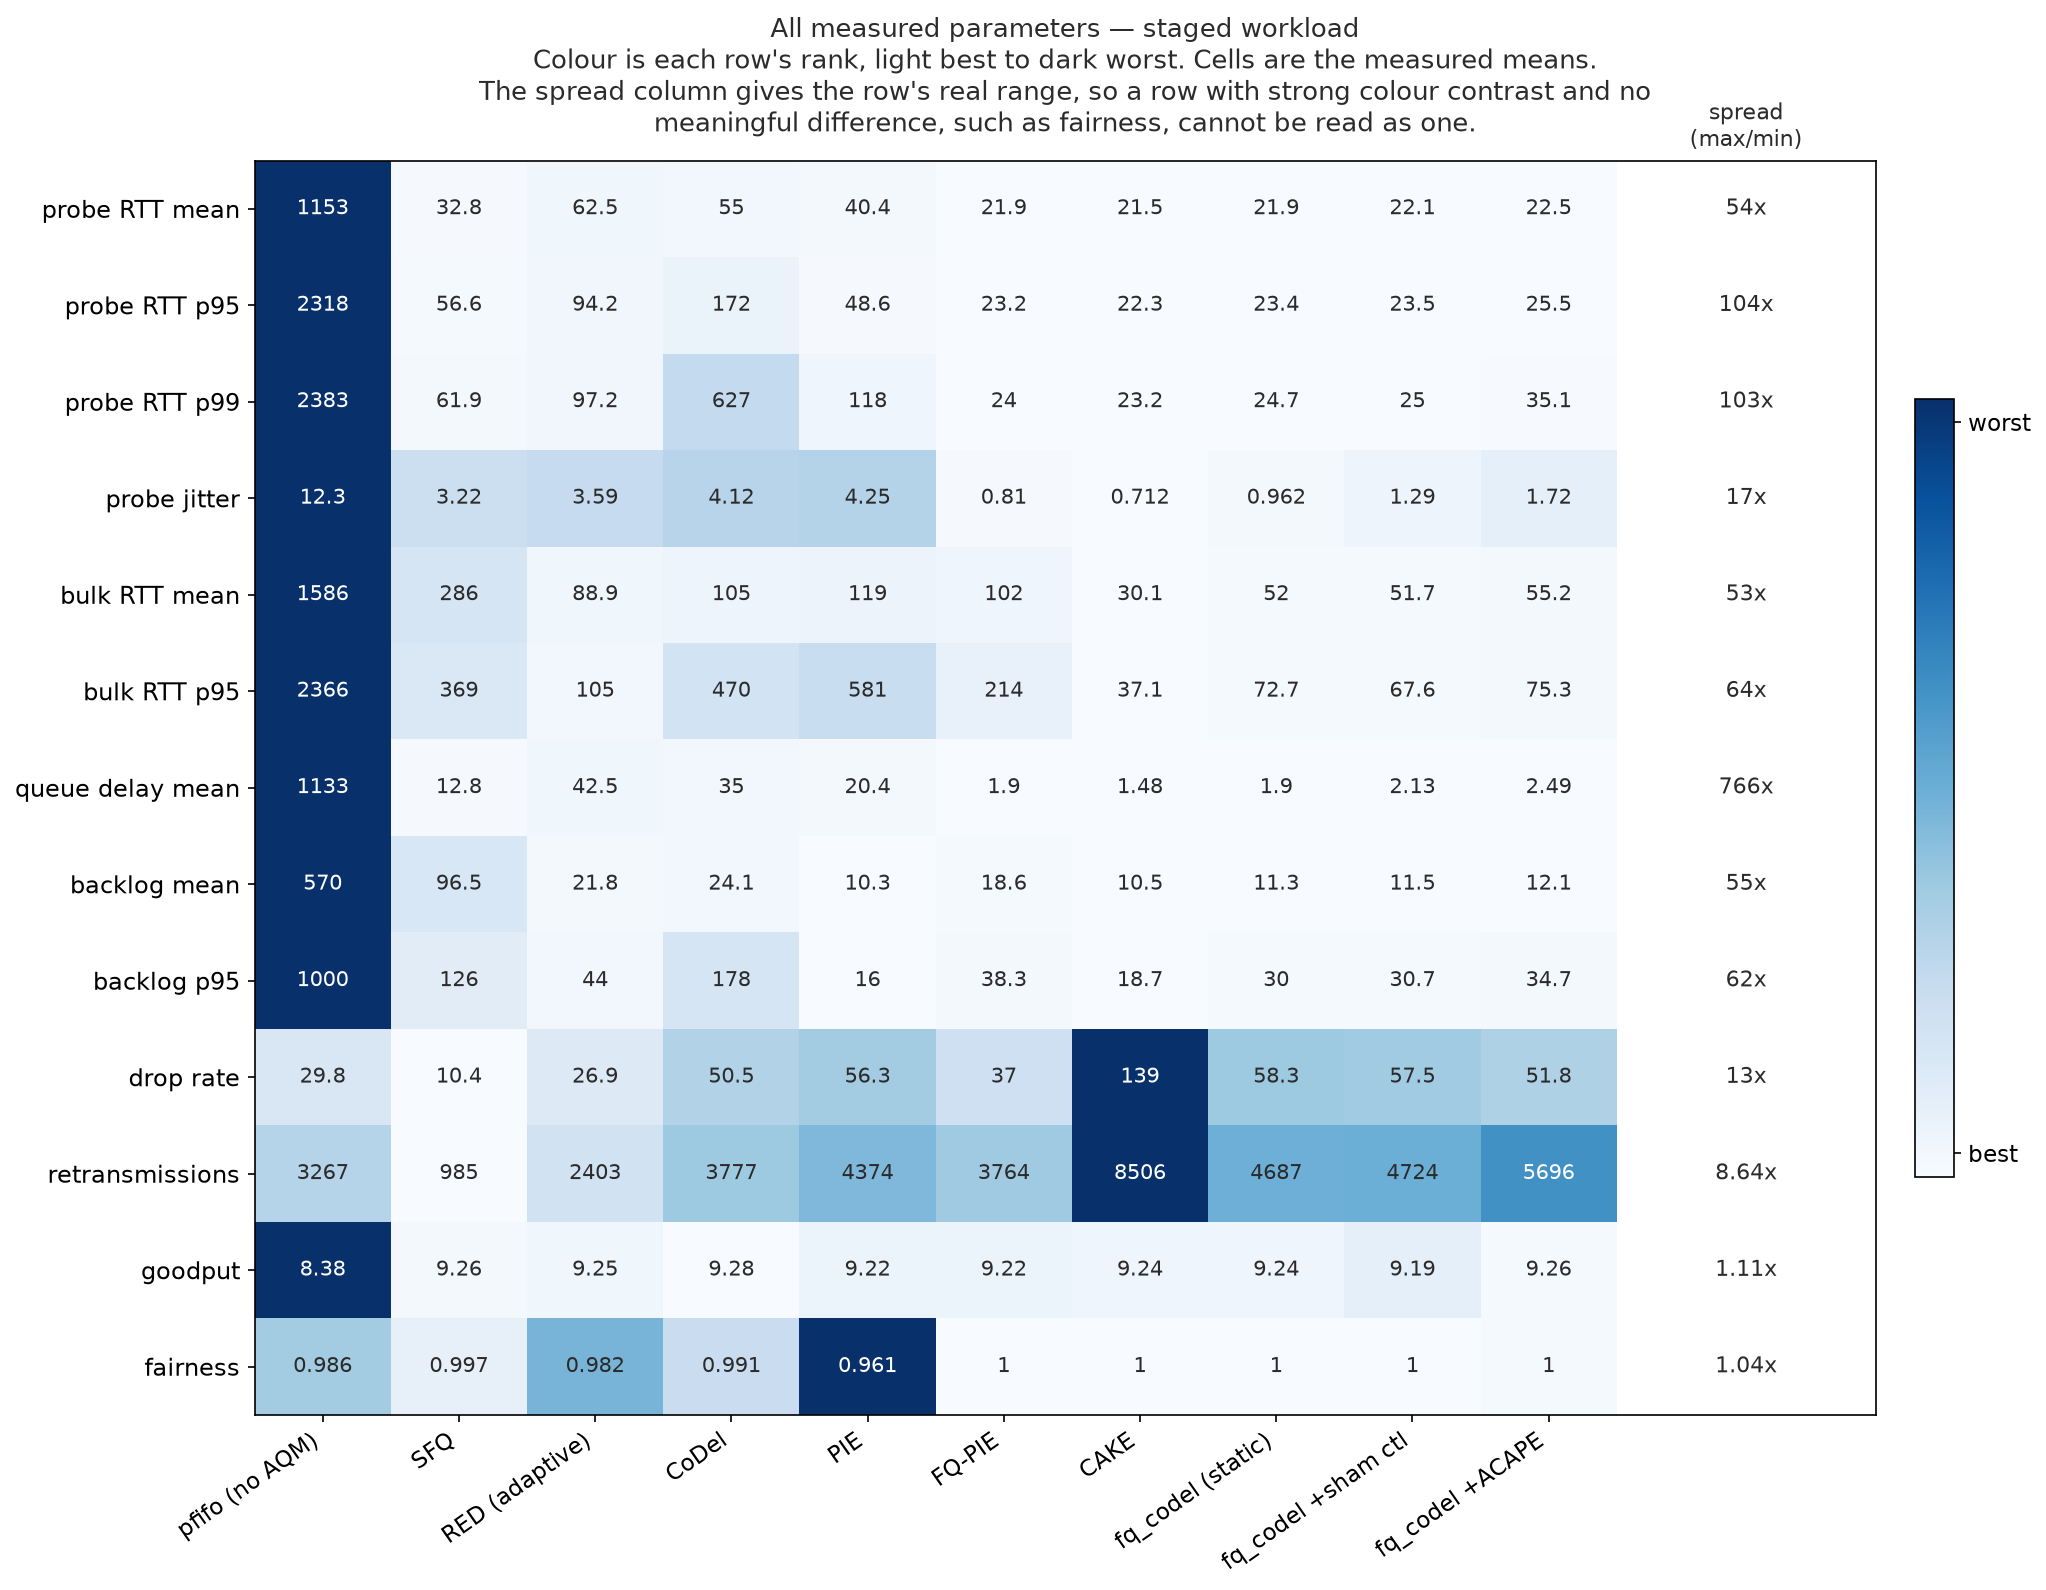
\includegraphics[width=\linewidth,height=0.42\textheight,keepaspectratio]{fig08_allparams_staged.png}
\caption{\textbf{FIG 15}: fig08\_allparams\_staged.png. All measured parameters × all systems, normalised heatmap with measured values (staged workload)}
\end{figure}

\begin{figure}[htbp]
\centering
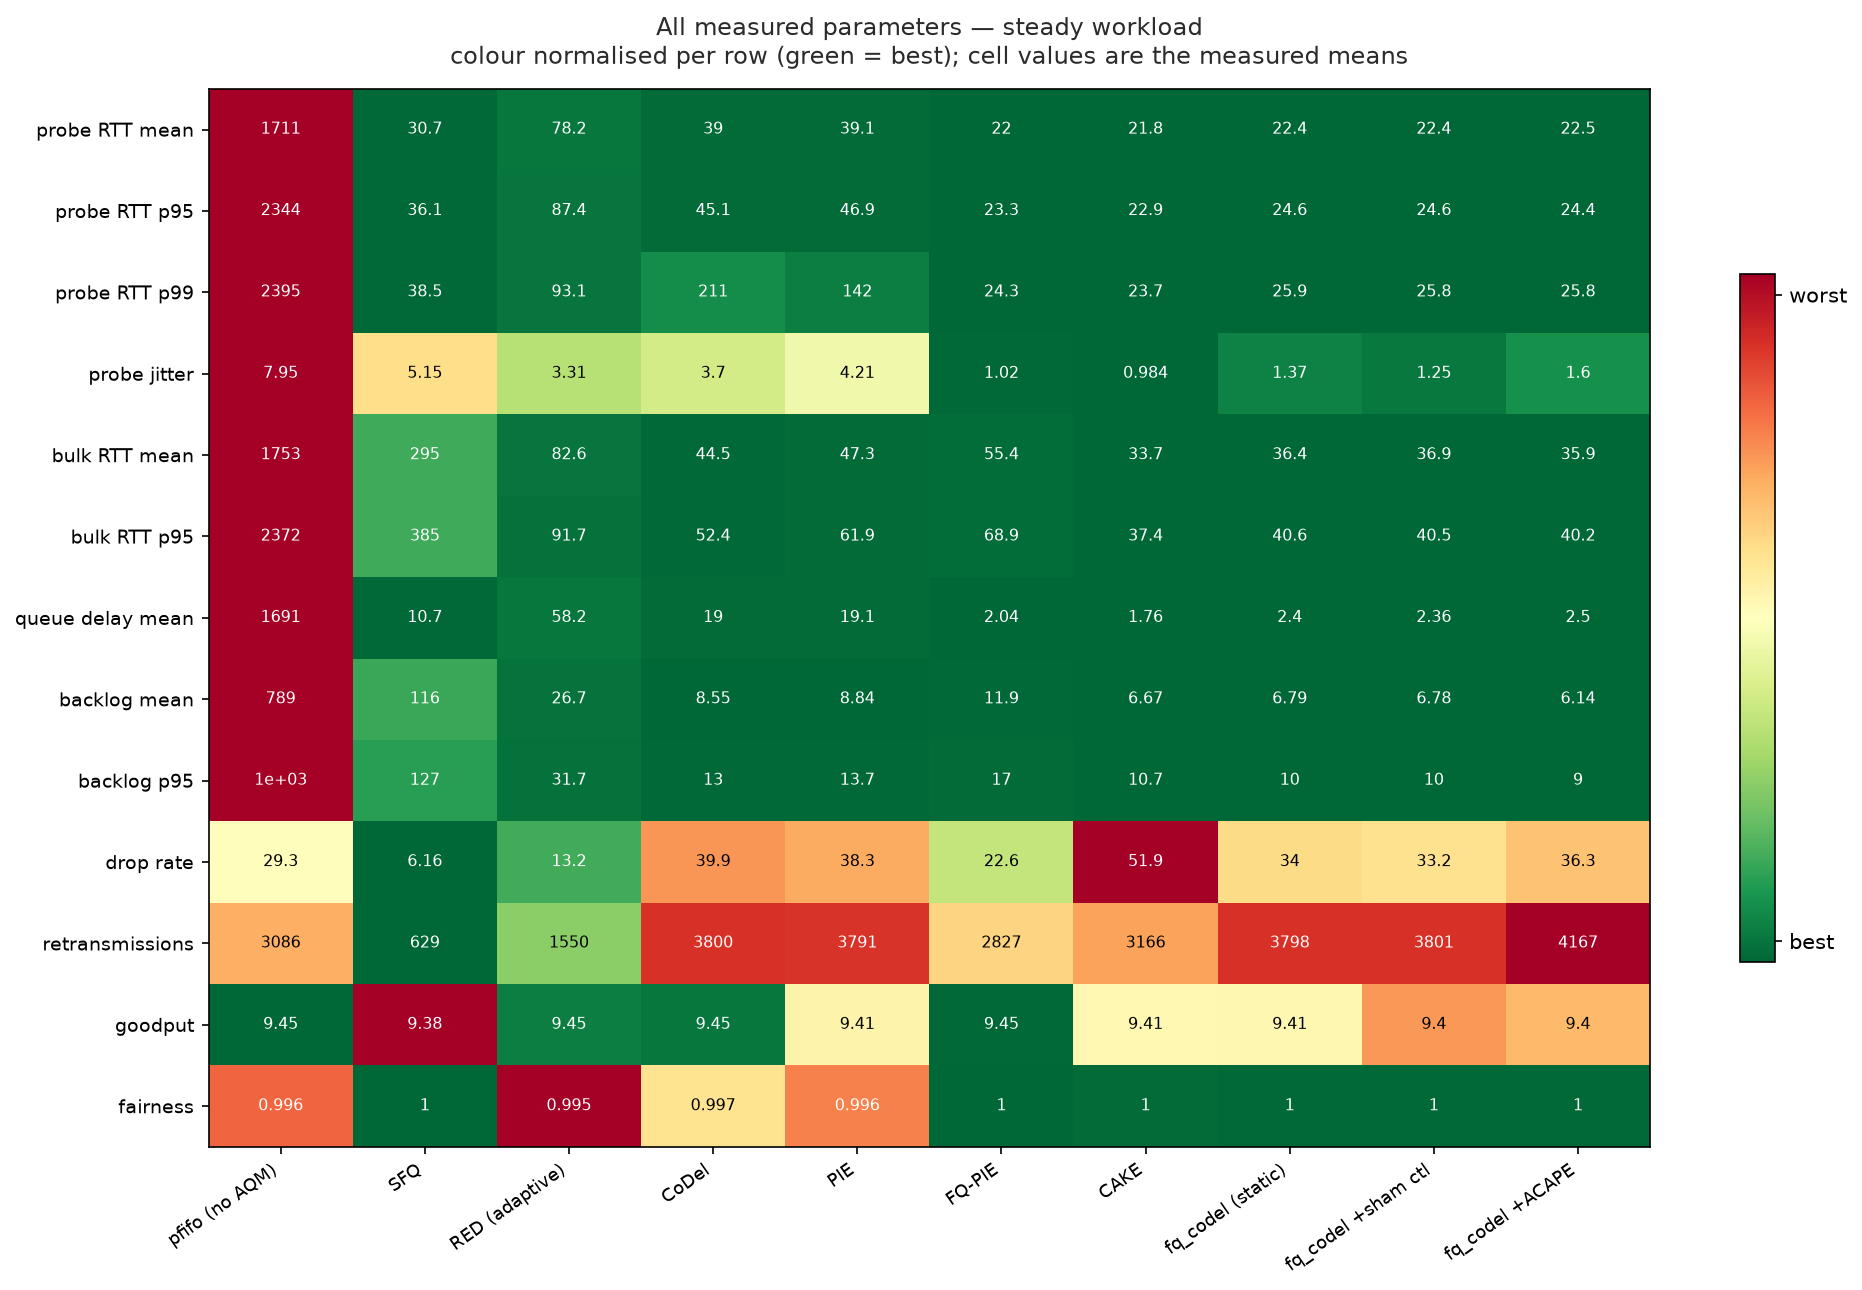
\includegraphics[width=\linewidth,height=0.42\textheight,keepaspectratio]{fig08_allparams_steady.png}
\caption{\textbf{FIG 16}: fig08\_allparams\_steady.png. All measured parameters × all systems, normalised heatmap with measured values (steady workload)}
\end{figure}

\begin{figure}[htbp]
\centering
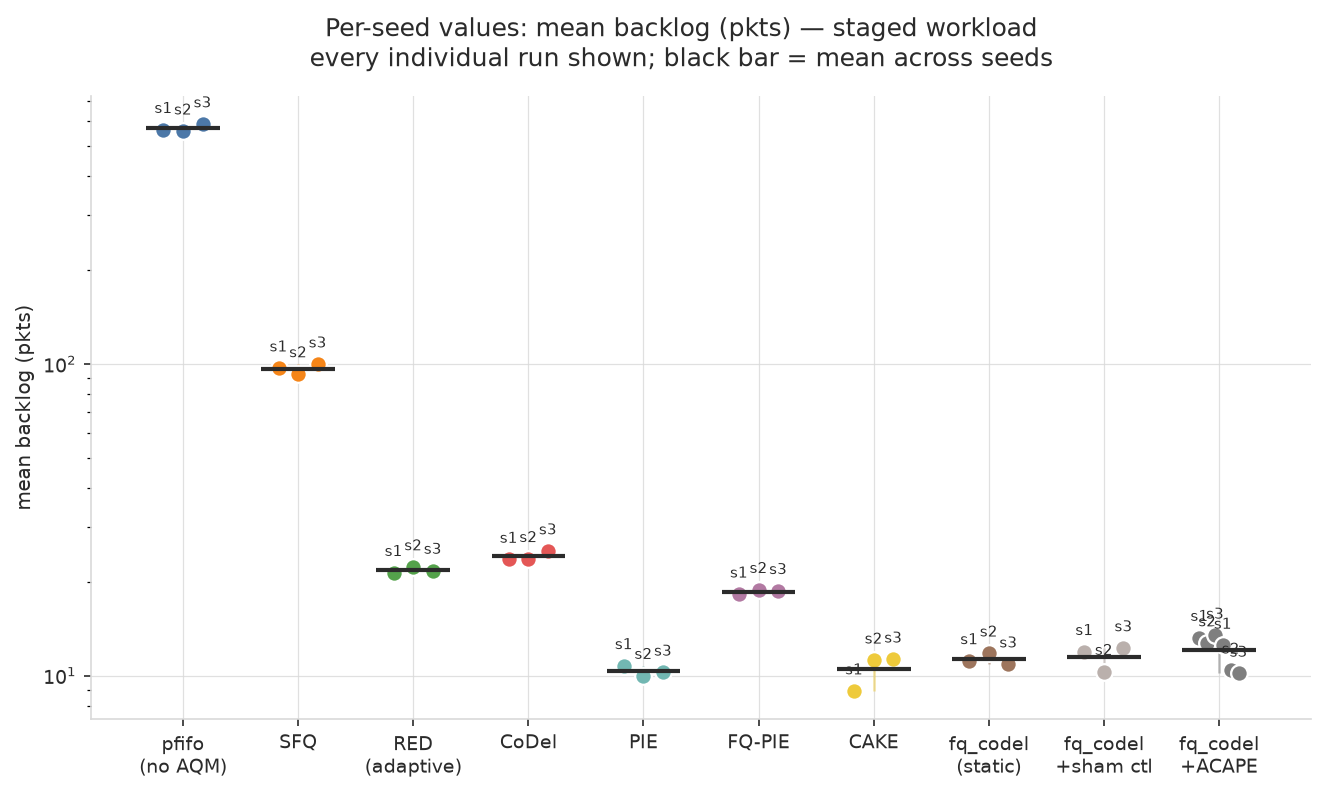
\includegraphics[width=\linewidth,height=0.42\textheight,keepaspectratio]{fig09_seeds_backlog_mean_pkts_staged.png}
\caption{\textbf{FIG 17}: fig09\_seeds\_backlog\_mean\_pkts\_staged.png. Per-seed values ,  every individual run shown, mean marked ,  backlog mean pkts (staged workload)}
\end{figure}

\begin{figure}[htbp]
\centering
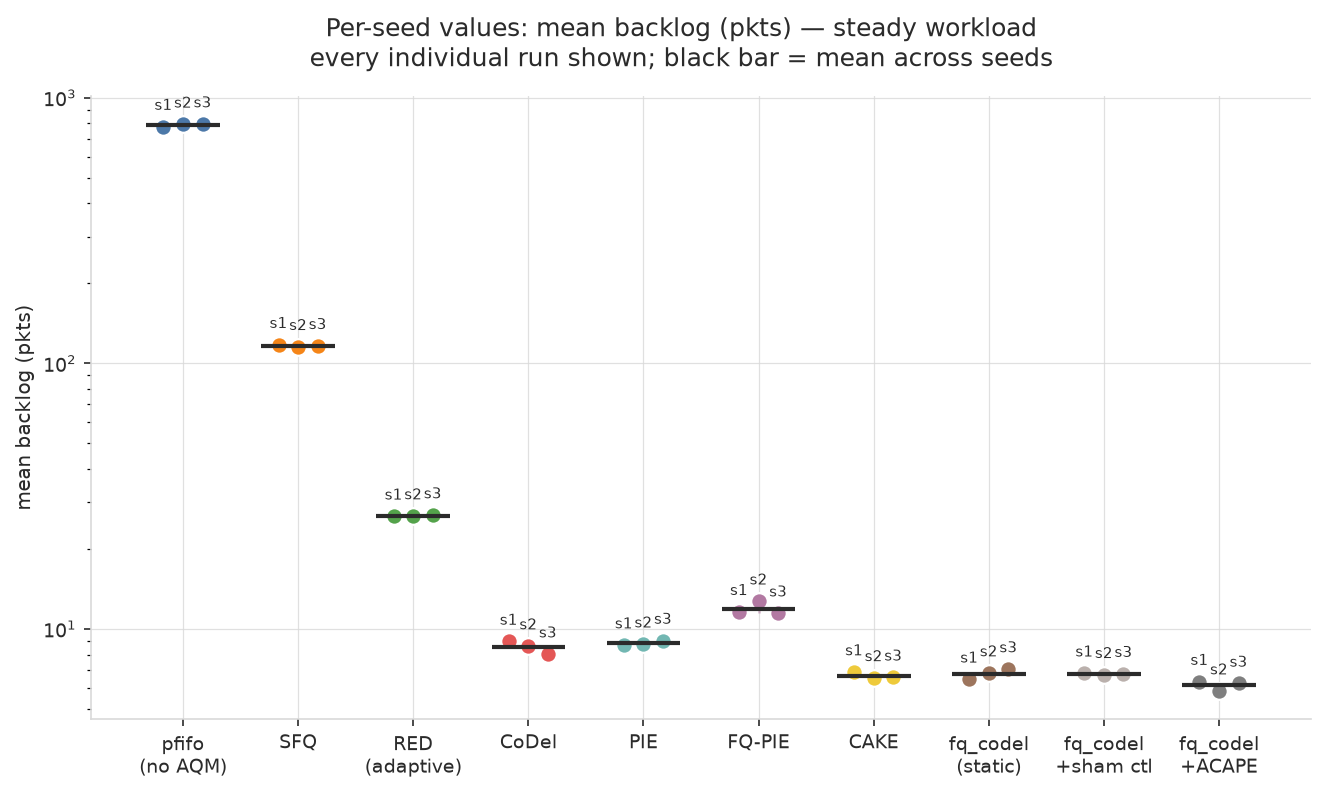
\includegraphics[width=\linewidth,height=0.42\textheight,keepaspectratio]{fig09_seeds_backlog_mean_pkts_steady.png}
\caption{\textbf{FIG 18}: fig09\_seeds\_backlog\_mean\_pkts\_steady.png. Per-seed values ,  every individual run shown, mean marked ,  backlog mean pkts (steady workload)}
\end{figure}

\begin{figure}[htbp]
\centering
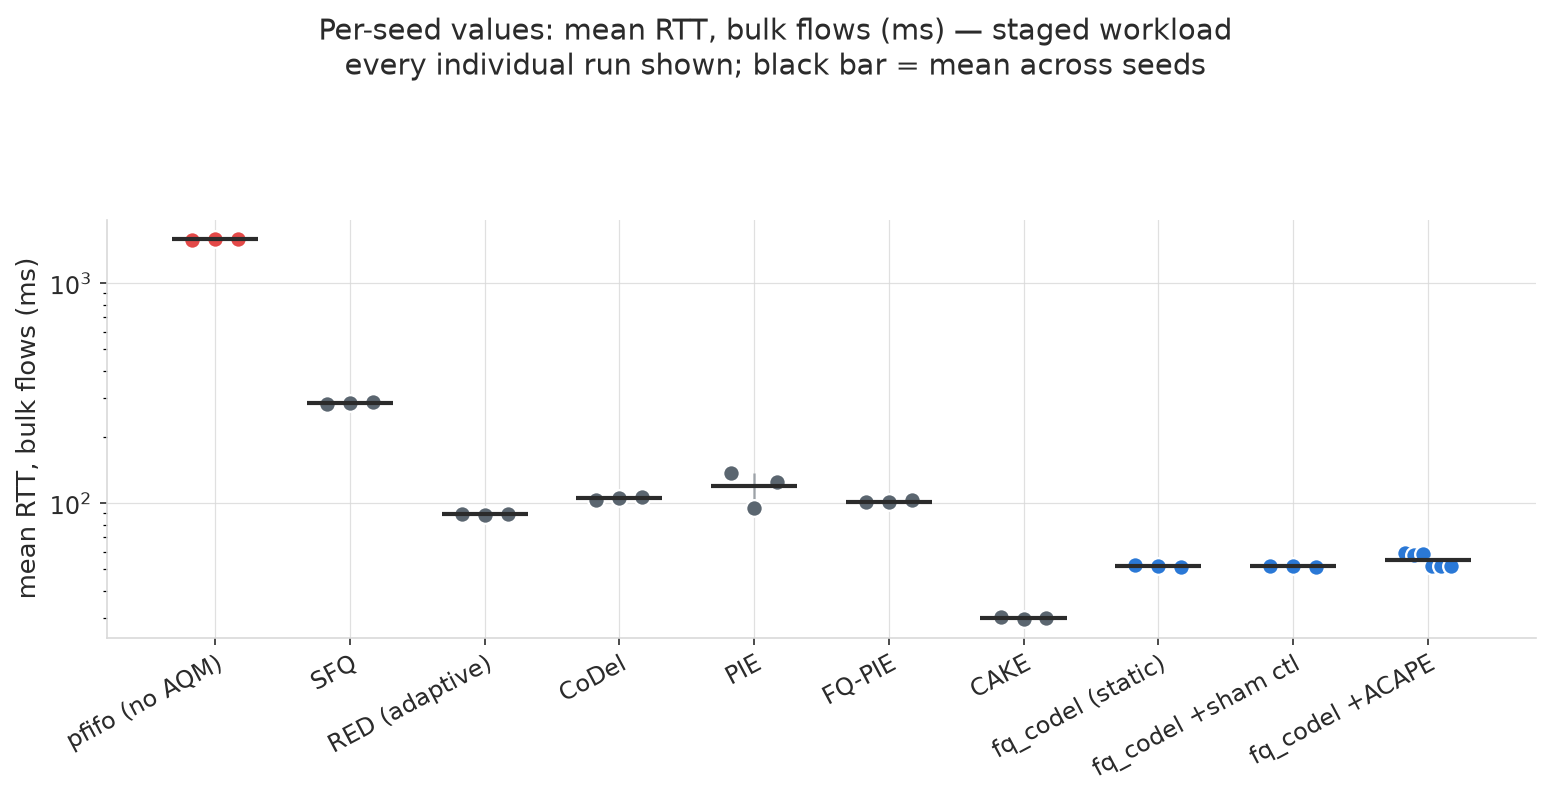
\includegraphics[width=\linewidth,height=0.42\textheight,keepaspectratio]{fig09_seeds_bulk_rtt_mean_ms_staged.png}
\caption{\textbf{FIG 19}: fig09\_seeds\_bulk\_rtt\_mean\_ms\_staged.png. Per-seed values ,  every individual run shown, mean marked ,  bulk rtt mean ms (staged workload)}
\end{figure}

\begin{figure}[htbp]
\centering
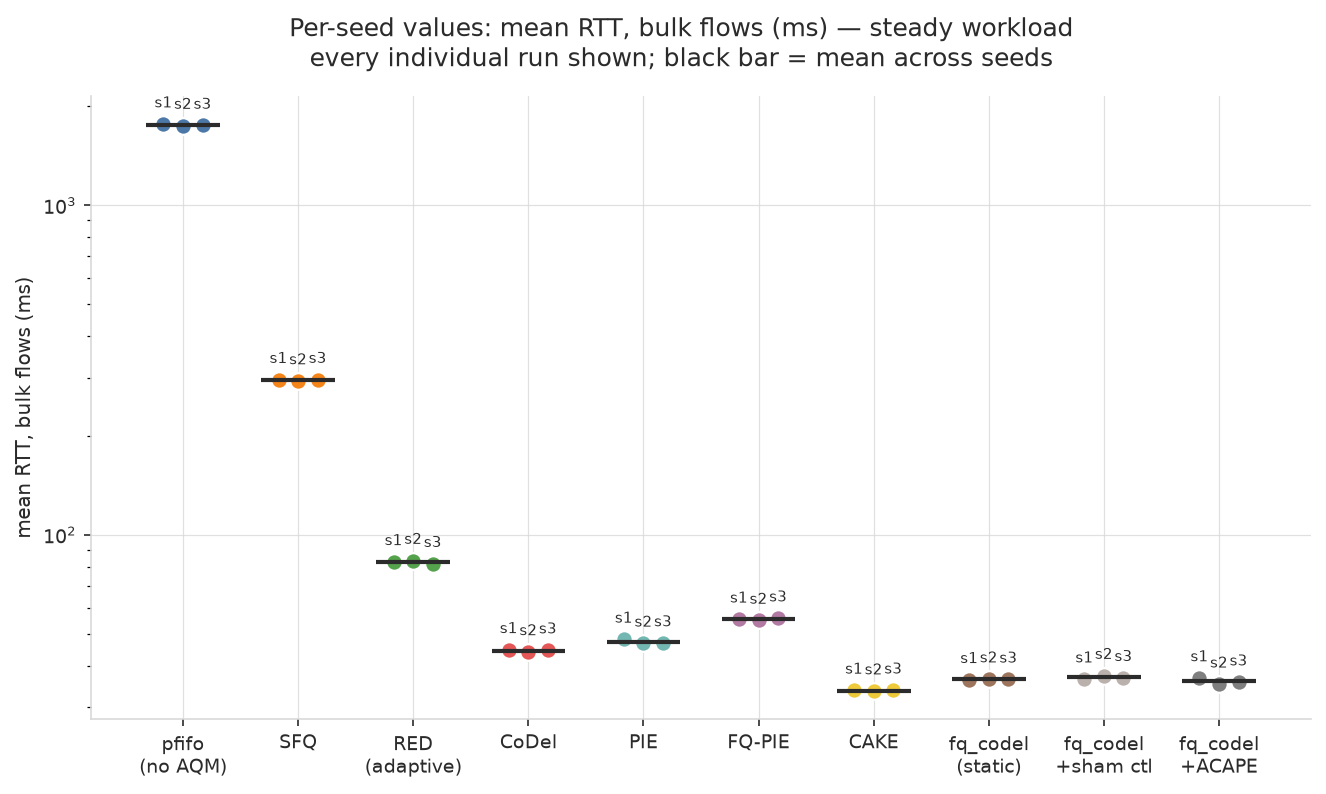
\includegraphics[width=\linewidth,height=0.42\textheight,keepaspectratio]{fig09_seeds_bulk_rtt_mean_ms_steady.png}
\caption{\textbf{FIG 20}: fig09\_seeds\_bulk\_rtt\_mean\_ms\_steady.png. Per-seed values ,  every individual run shown, mean marked ,  bulk rtt mean ms (steady workload)}
\end{figure}

\begin{figure}[htbp]
\centering
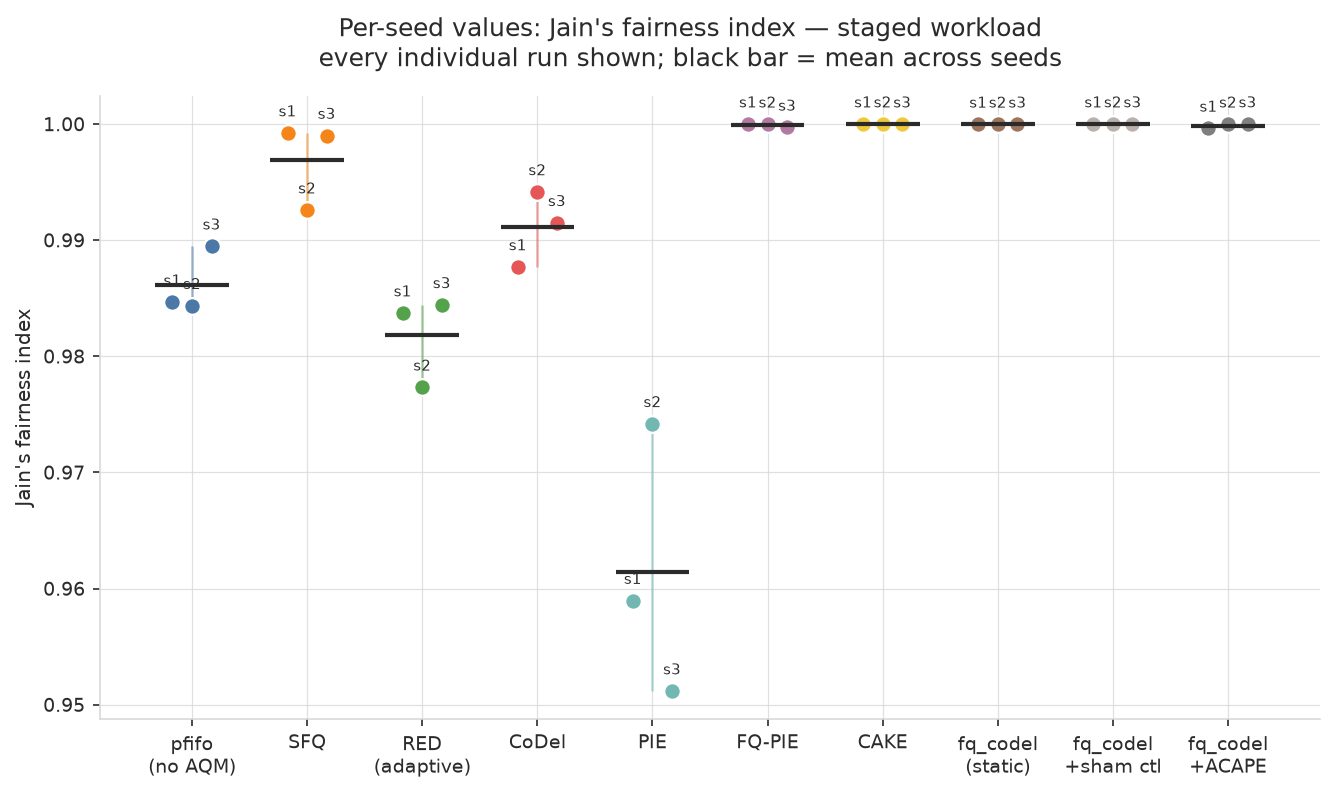
\includegraphics[width=\linewidth,height=0.42\textheight,keepaspectratio]{fig09_seeds_jain_staged.png}
\caption{\textbf{FIG 21}: fig09\_seeds\_jain\_staged.png. Per-seed values ,  every individual run shown, mean marked ,  jain (staged workload)}
\end{figure}

\begin{figure}[htbp]
\centering
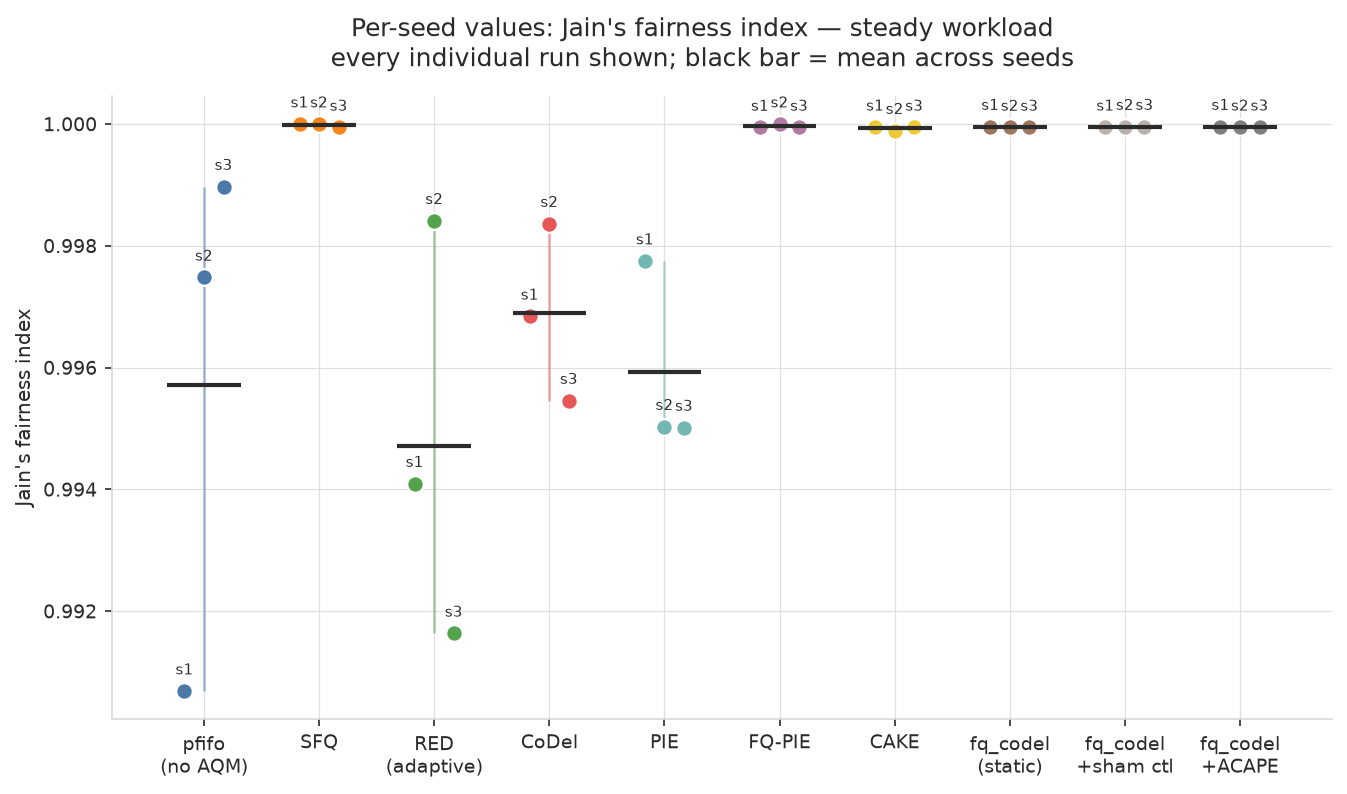
\includegraphics[width=\linewidth,height=0.42\textheight,keepaspectratio]{fig09_seeds_jain_steady.png}
\caption{\textbf{FIG 22}: fig09\_seeds\_jain\_steady.png. Per-seed values ,  every individual run shown, mean marked ,  jain (steady workload)}
\end{figure}

\begin{figure}[htbp]
\centering
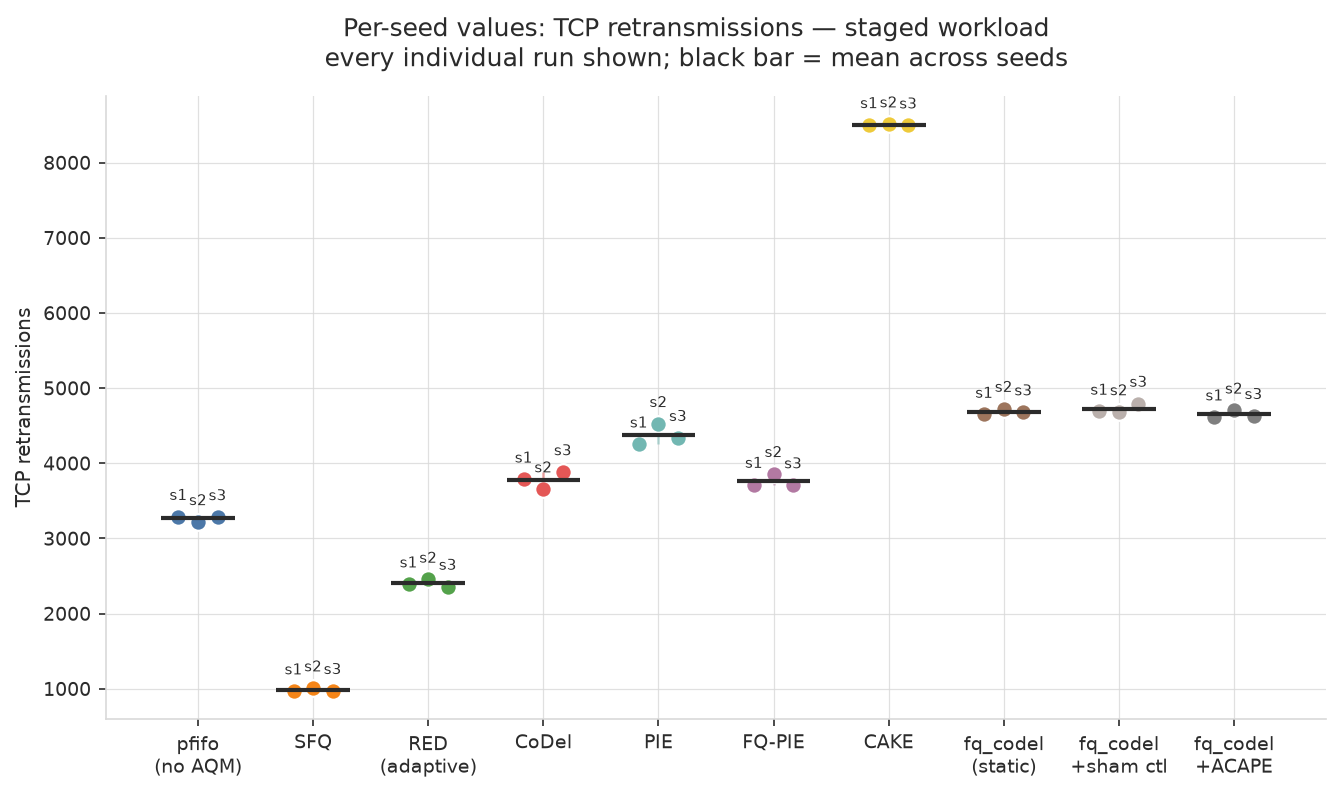
\includegraphics[width=\linewidth,height=0.42\textheight,keepaspectratio]{fig09_seeds_retransmits_staged.png}
\caption{\textbf{FIG 23}: fig09\_seeds\_retransmits\_staged.png. Per-seed values ,  every individual run shown, mean marked ,  retransmits (staged workload)}
\end{figure}

\begin{figure}[htbp]
\centering
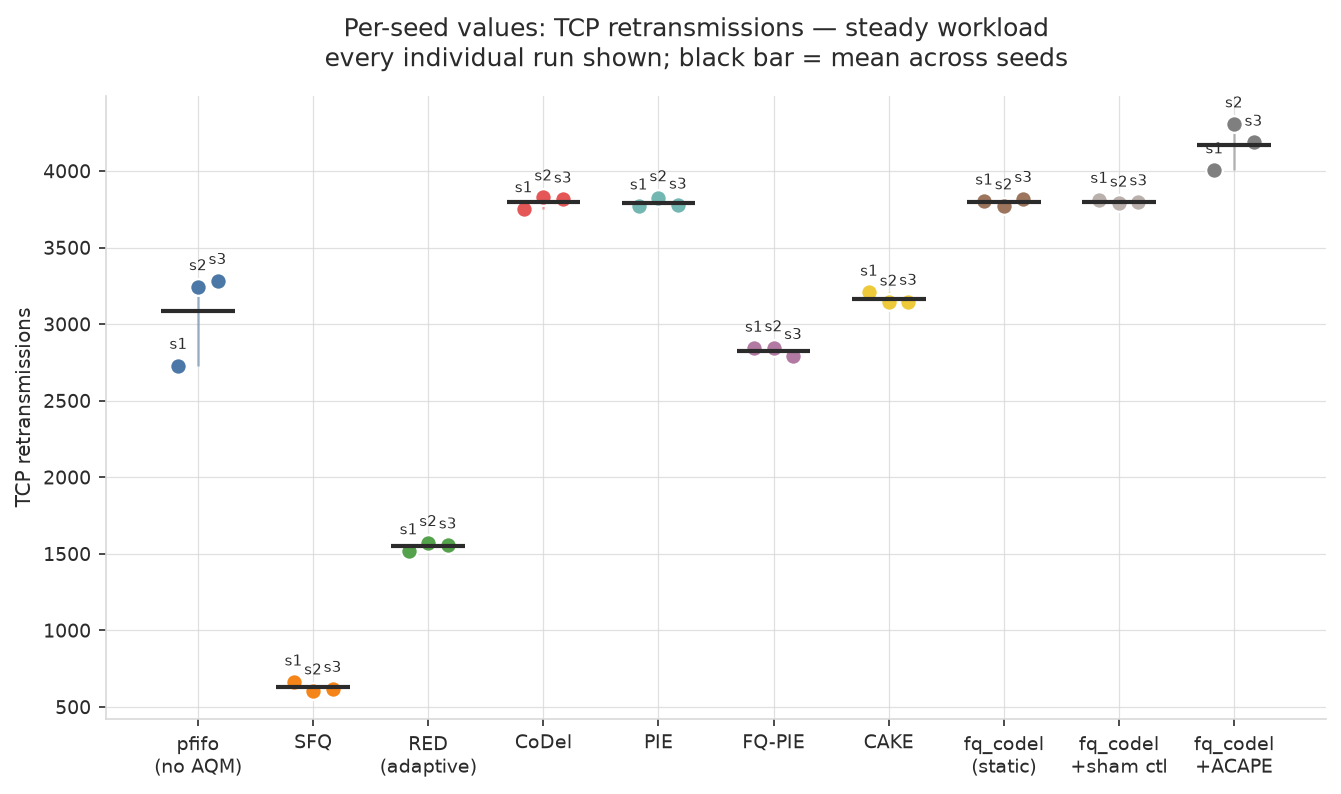
\includegraphics[width=\linewidth,height=0.42\textheight,keepaspectratio]{fig09_seeds_retransmits_steady.png}
\caption{\textbf{FIG 24}: fig09\_seeds\_retransmits\_steady.png. Per-seed values ,  every individual run shown, mean marked ,  retransmits (steady workload)}
\end{figure}

\begin{figure}[htbp]
\centering
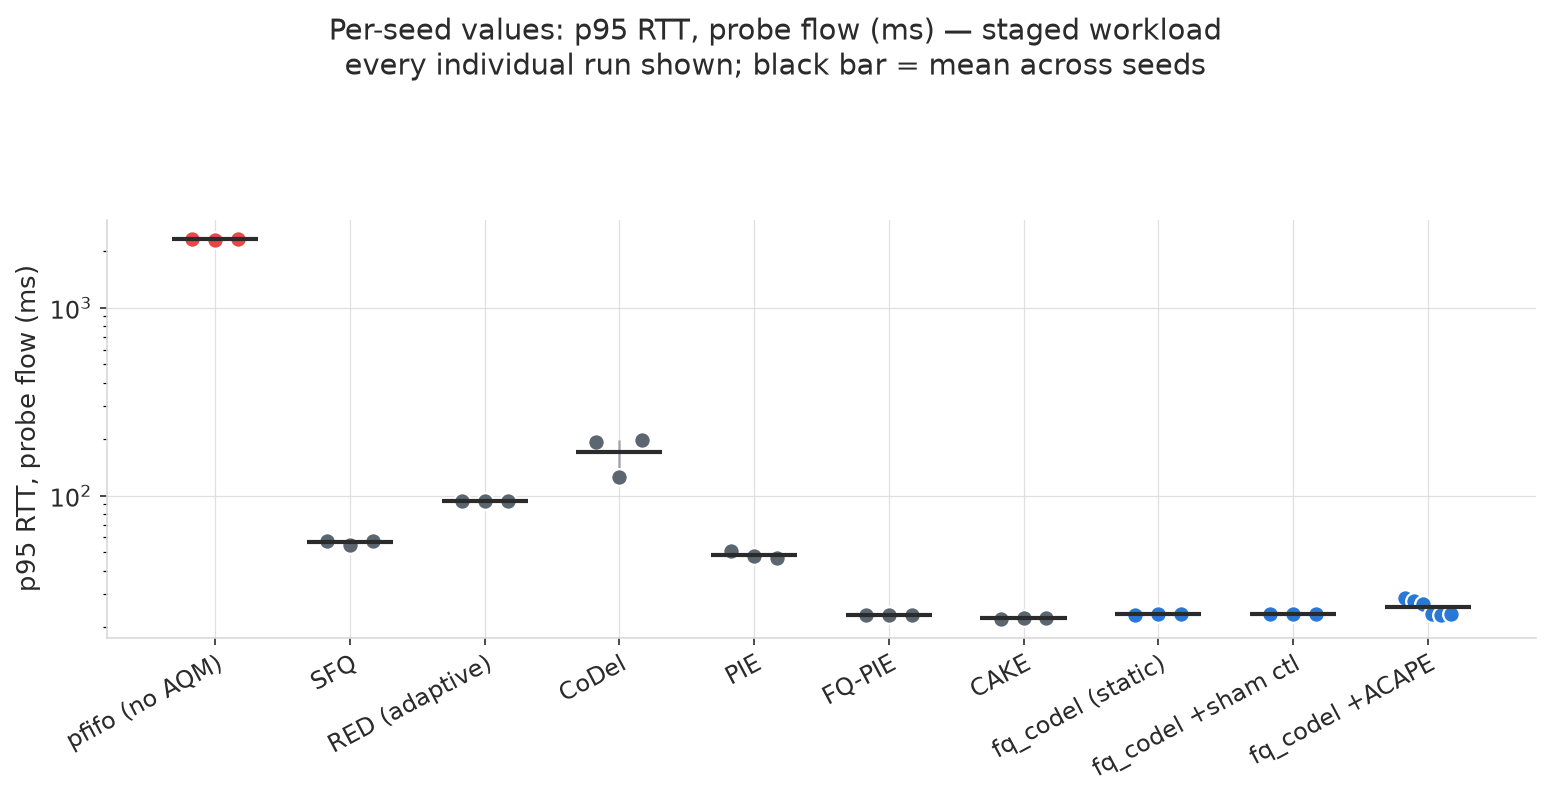
\includegraphics[width=\linewidth,height=0.42\textheight,keepaspectratio]{fig09_seeds_sparse_rtt_p95_ms_staged.png}
\caption{\textbf{FIG 25}: fig09\_seeds\_sparse\_rtt\_p95\_ms\_staged.png. Per-seed values ,  every individual run shown, mean marked ,  sparse rtt p95 ms (staged workload)}
\end{figure}

\begin{figure}[htbp]
\centering
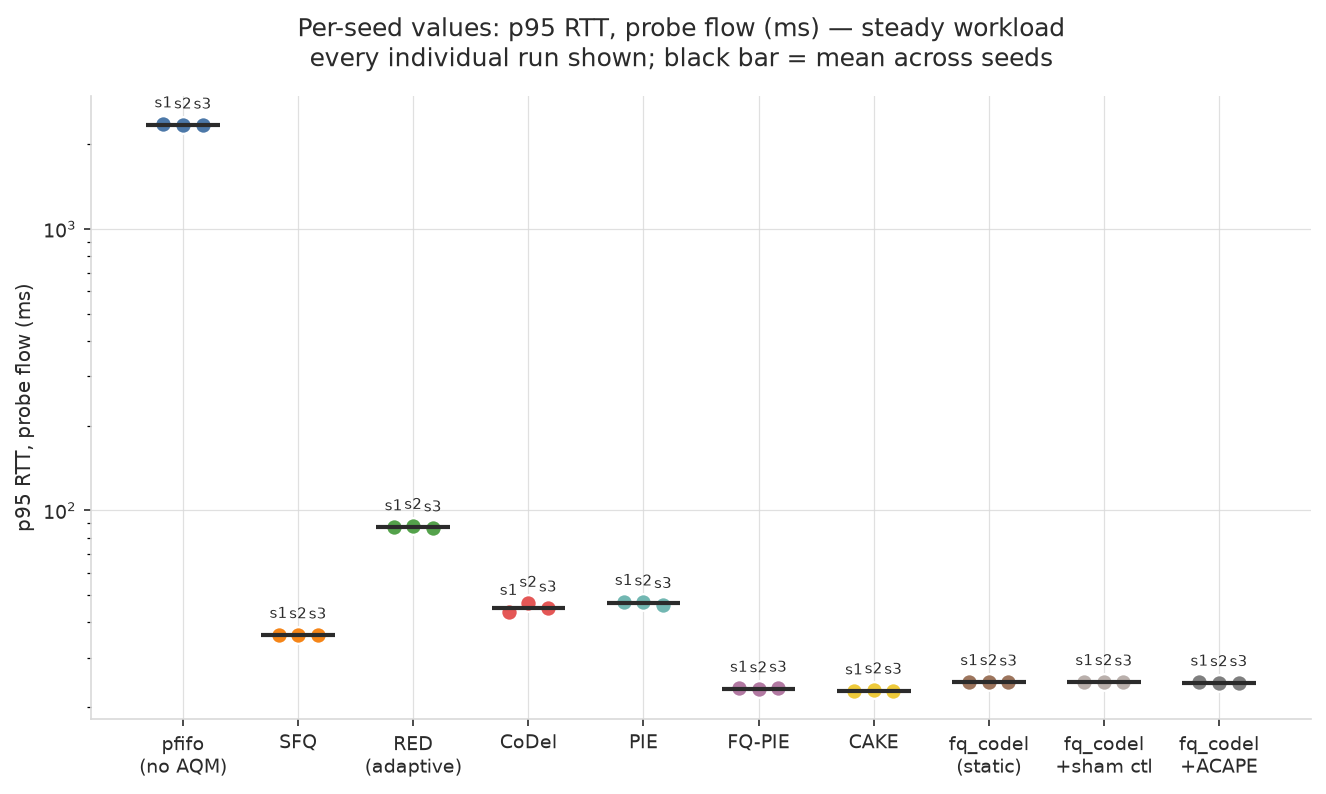
\includegraphics[width=\linewidth,height=0.42\textheight,keepaspectratio]{fig09_seeds_sparse_rtt_p95_ms_steady.png}
\caption{\textbf{FIG 26}: fig09\_seeds\_sparse\_rtt\_p95\_ms\_steady.png. Per-seed values ,  every individual run shown, mean marked ,  sparse rtt p95 ms (steady workload)}
\end{figure}

\begin{figure}[htbp]
\centering
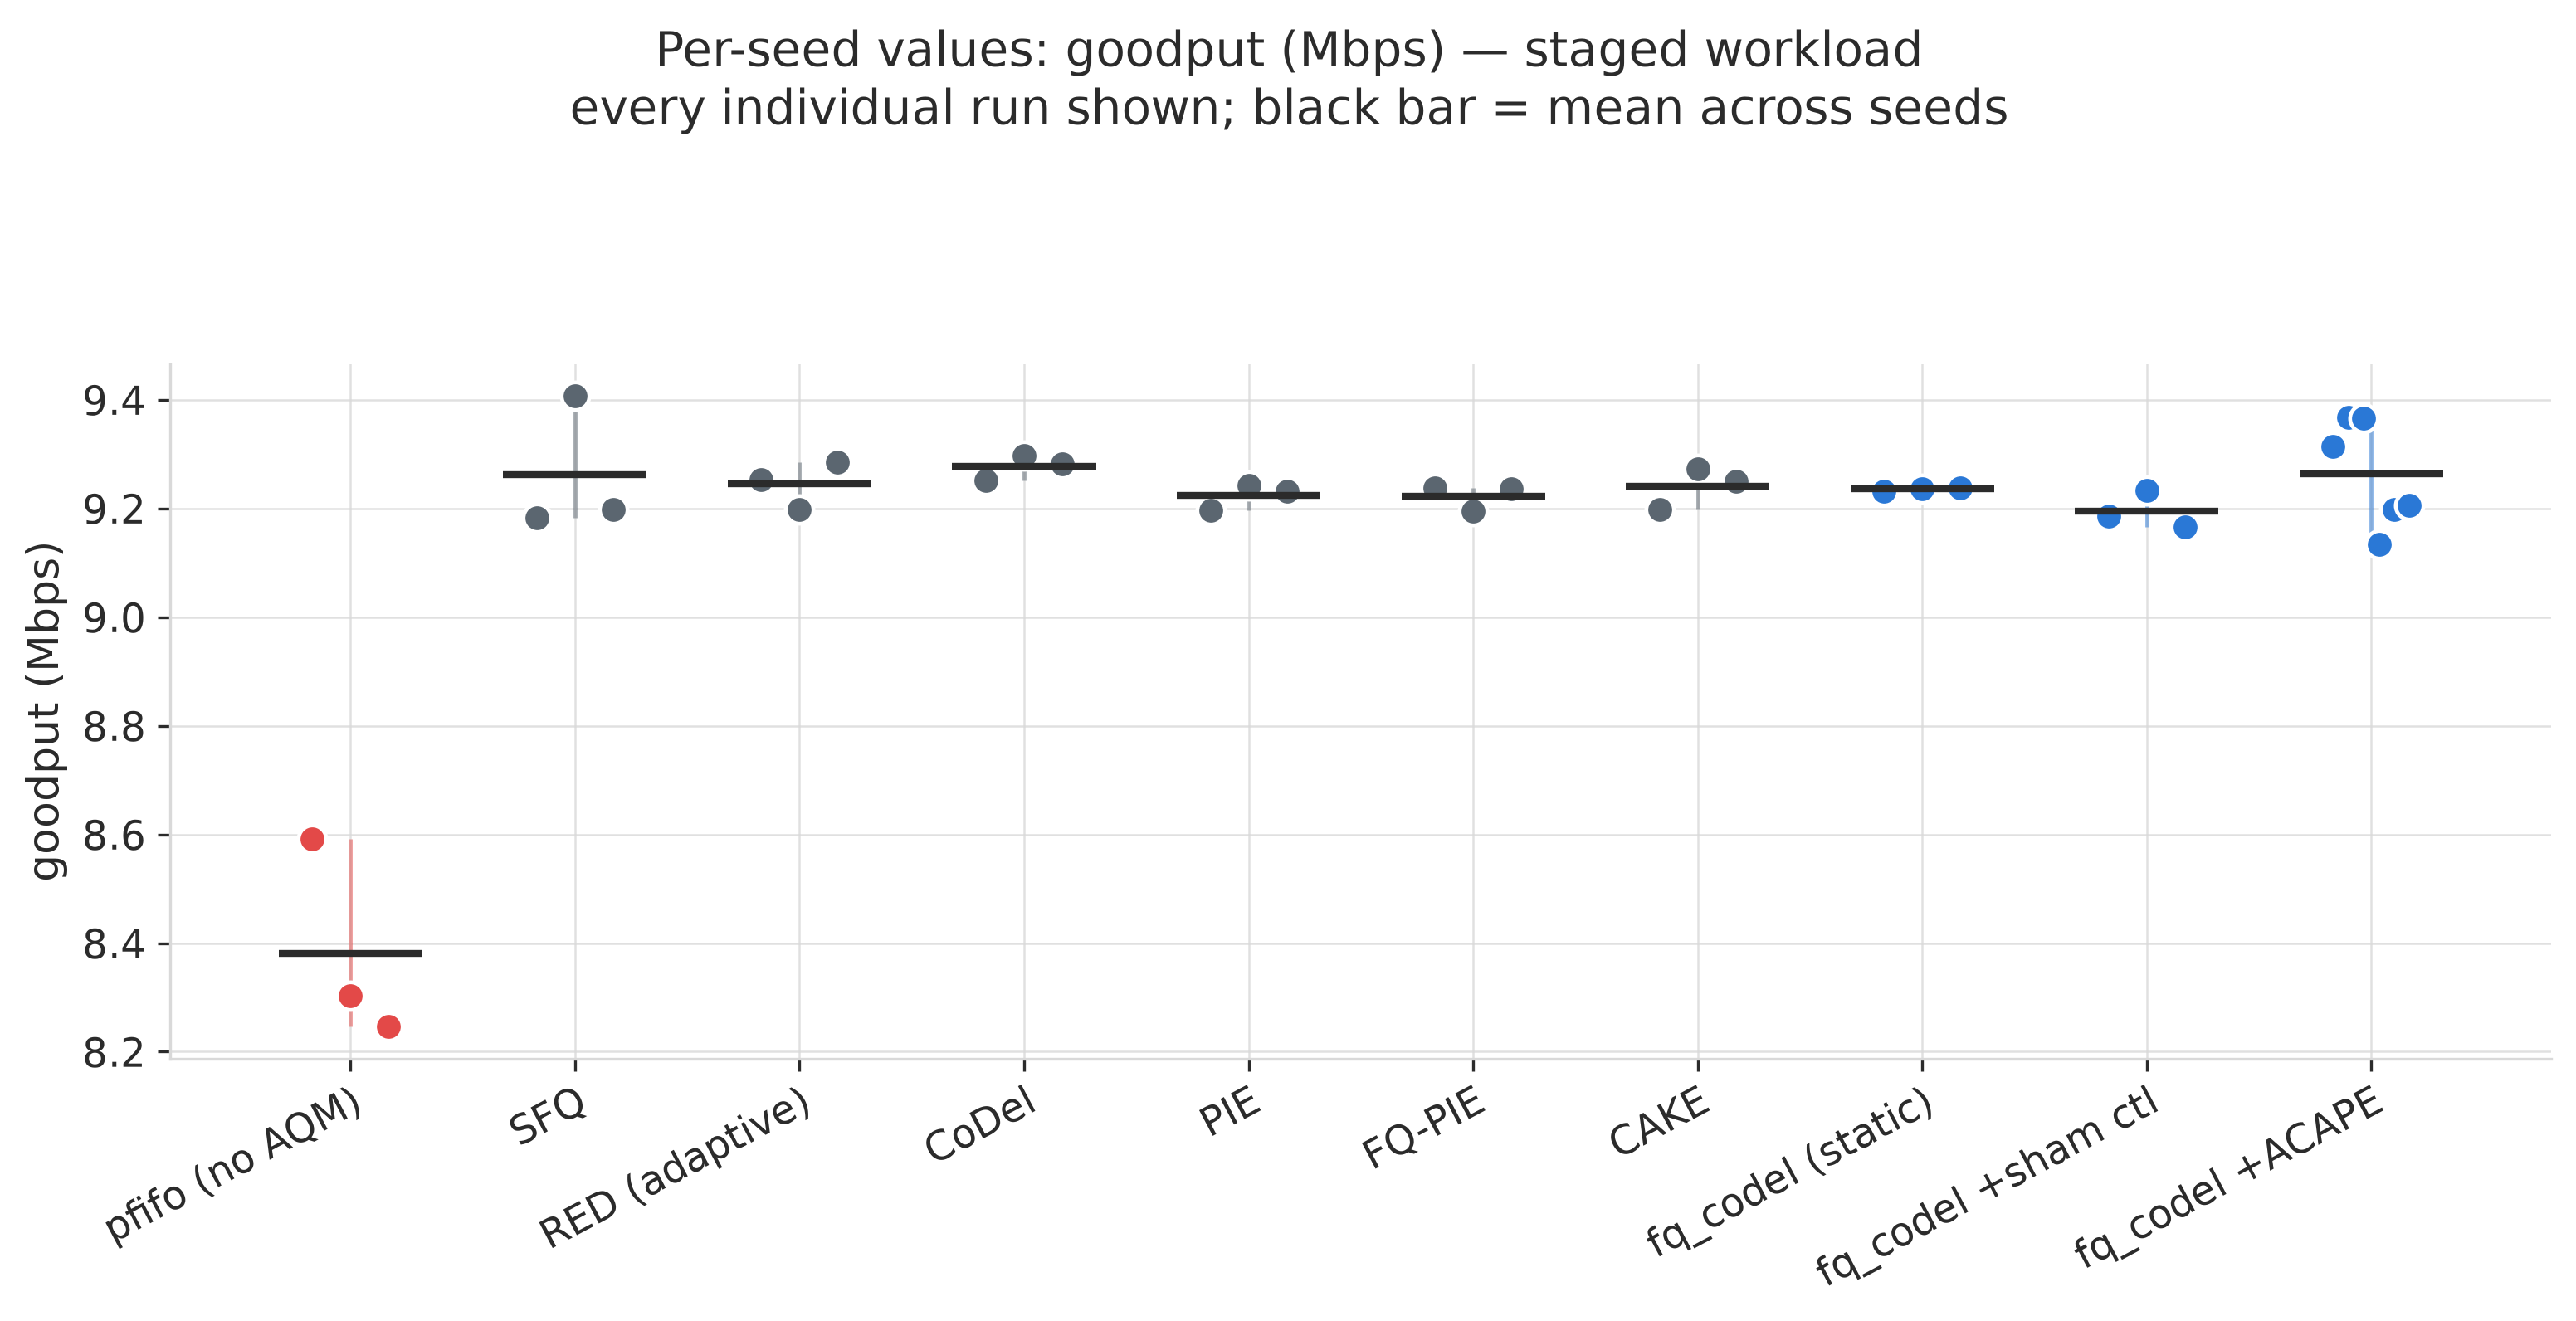
\includegraphics[width=\linewidth,height=0.42\textheight,keepaspectratio]{fig09_seeds_throughput_mbps_staged.png}
\caption{\textbf{FIG 27}: fig09\_seeds\_throughput\_mbps\_staged.png. Per-seed values ,  every individual run shown, mean marked ,  throughput mbps (staged workload)}
\end{figure}

\begin{figure}[htbp]
\centering
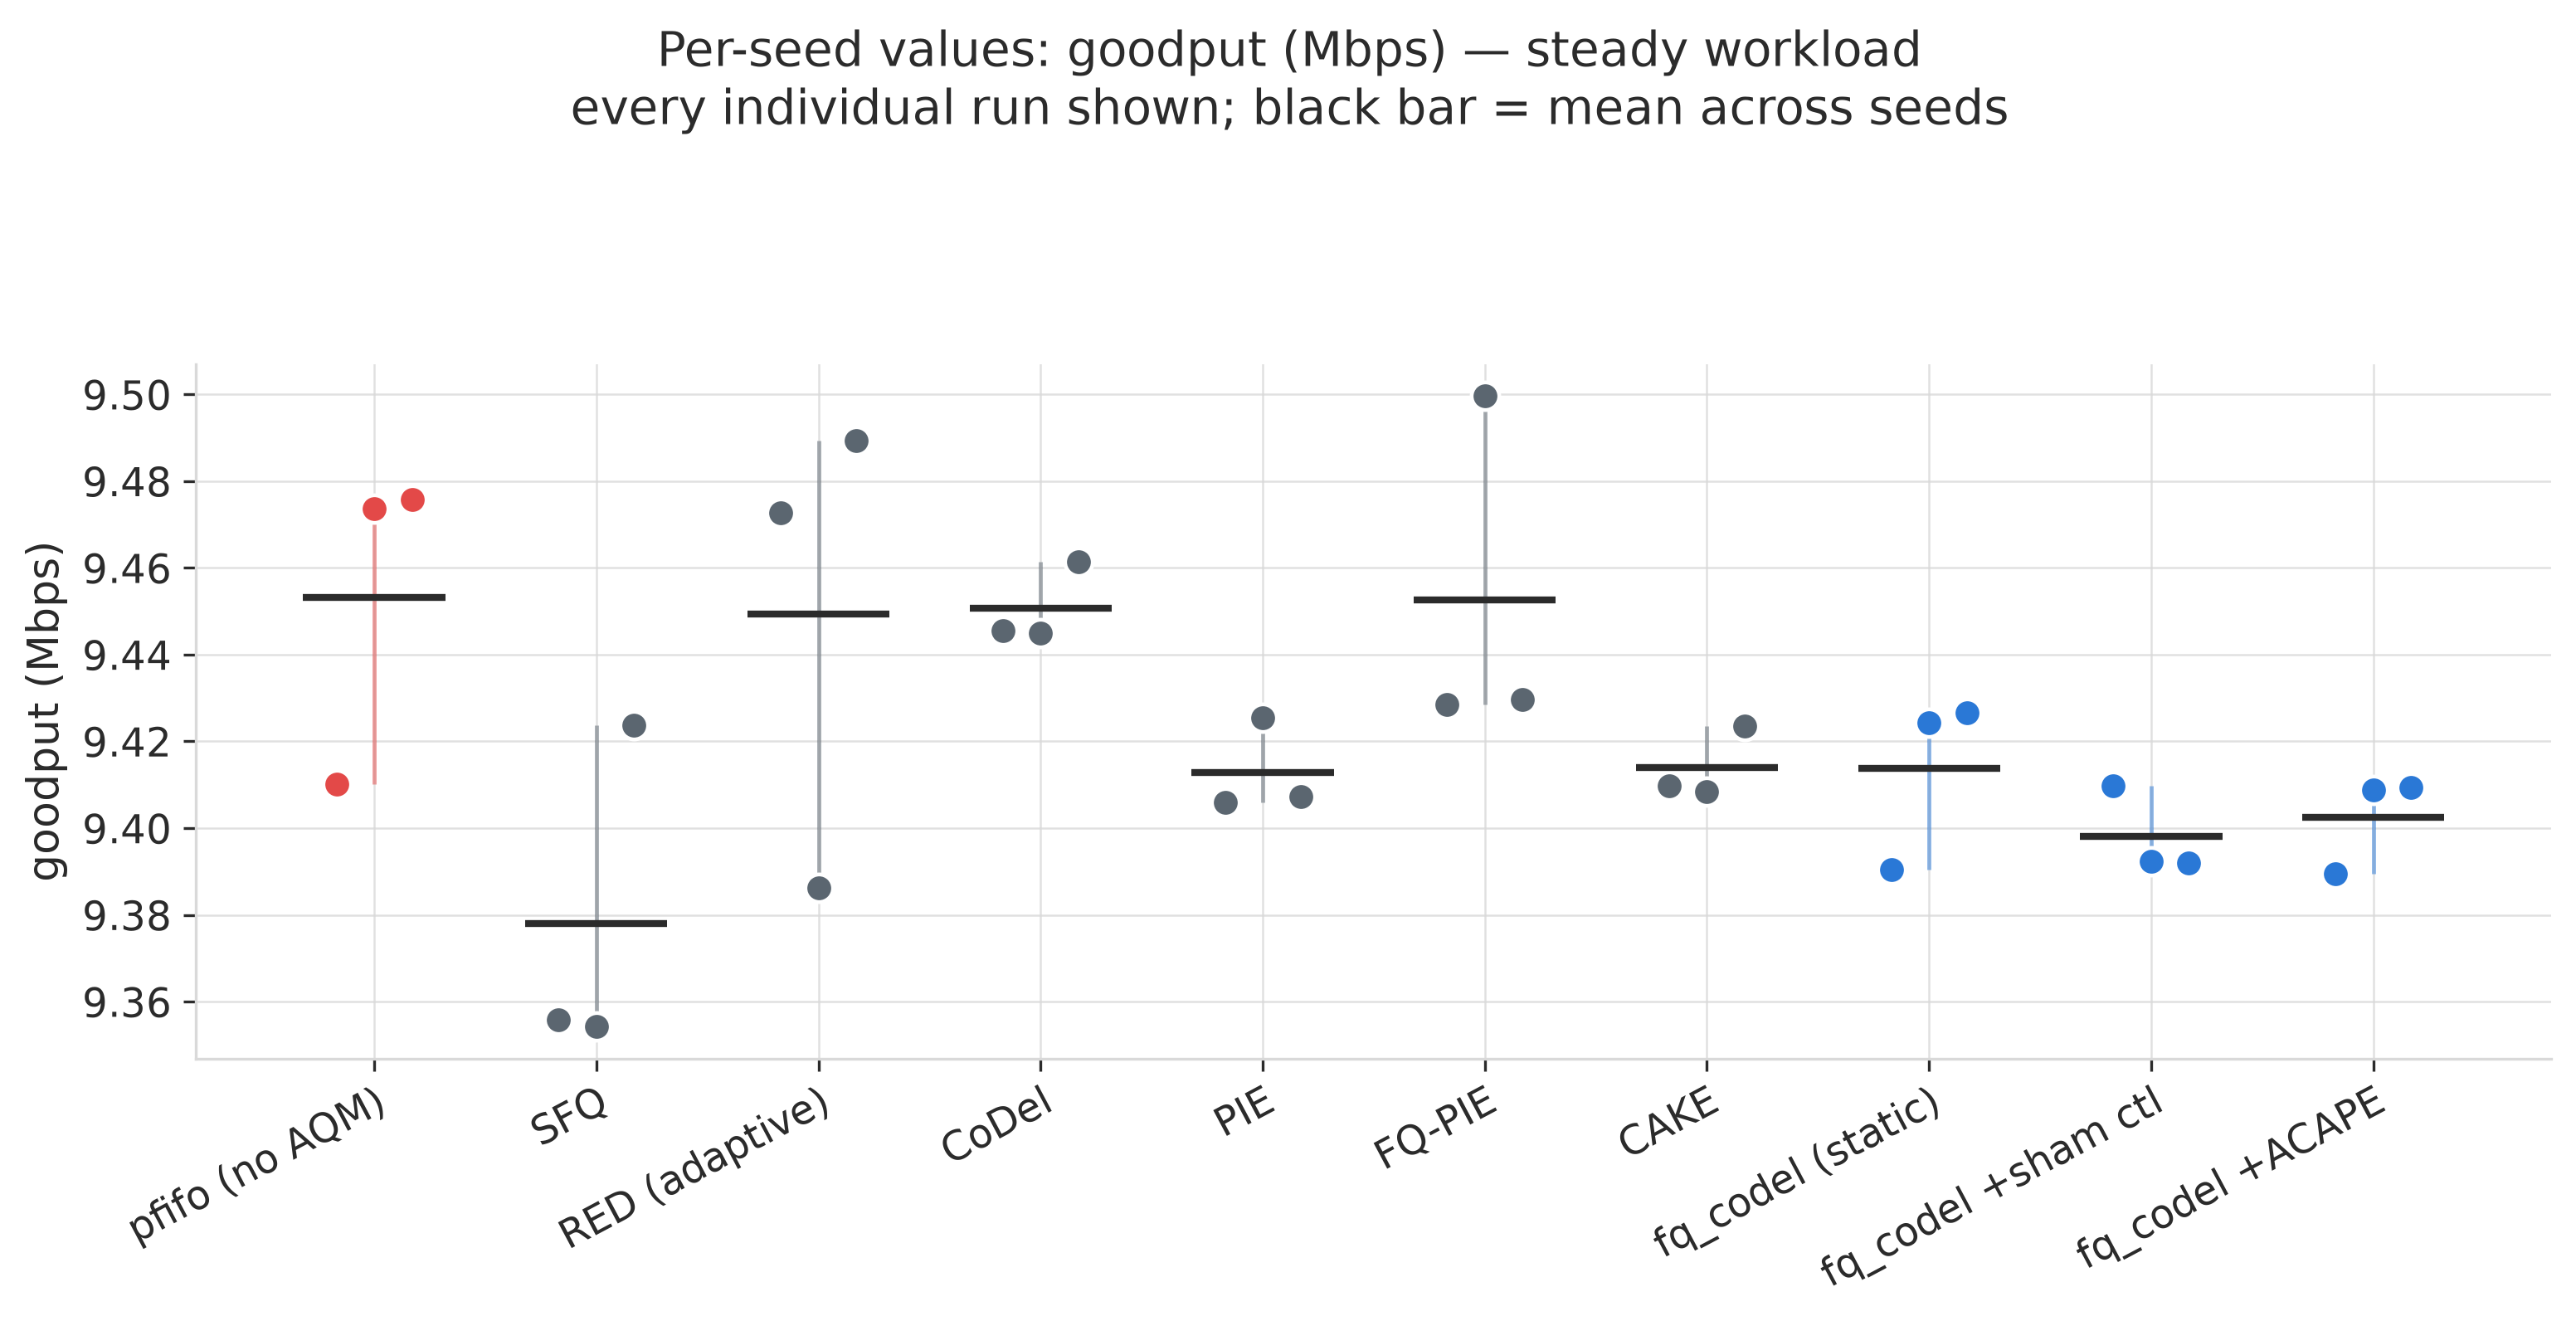
\includegraphics[width=\linewidth,height=0.42\textheight,keepaspectratio]{fig09_seeds_throughput_mbps_steady.png}
\caption{\textbf{FIG 28}: fig09\_seeds\_throughput\_mbps\_steady.png. Per-seed values ,  every individual run shown, mean marked ,  throughput mbps (steady workload)}
\end{figure}

\begin{figure}[htbp]
\centering
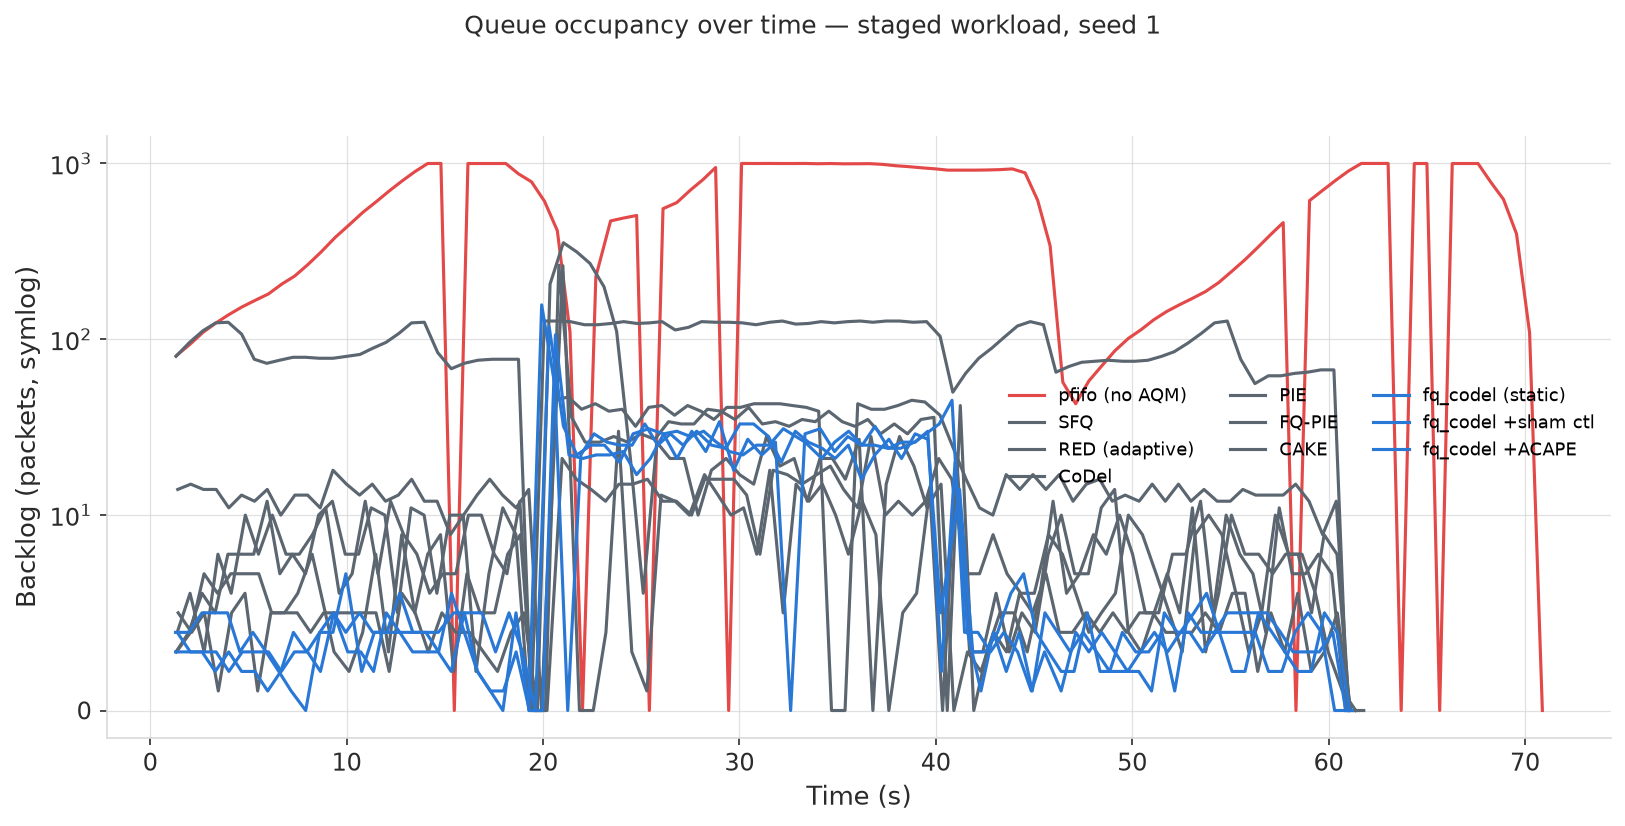
\includegraphics[width=\linewidth,height=0.42\textheight,keepaspectratio]{fig10_timeseries_backlog_staged.png}
\caption{\textbf{FIG 29}: fig10\_timeseries\_backlog\_staged.png. Queue occupancy over time (staged workload)}
\end{figure}

\begin{figure}[htbp]
\centering
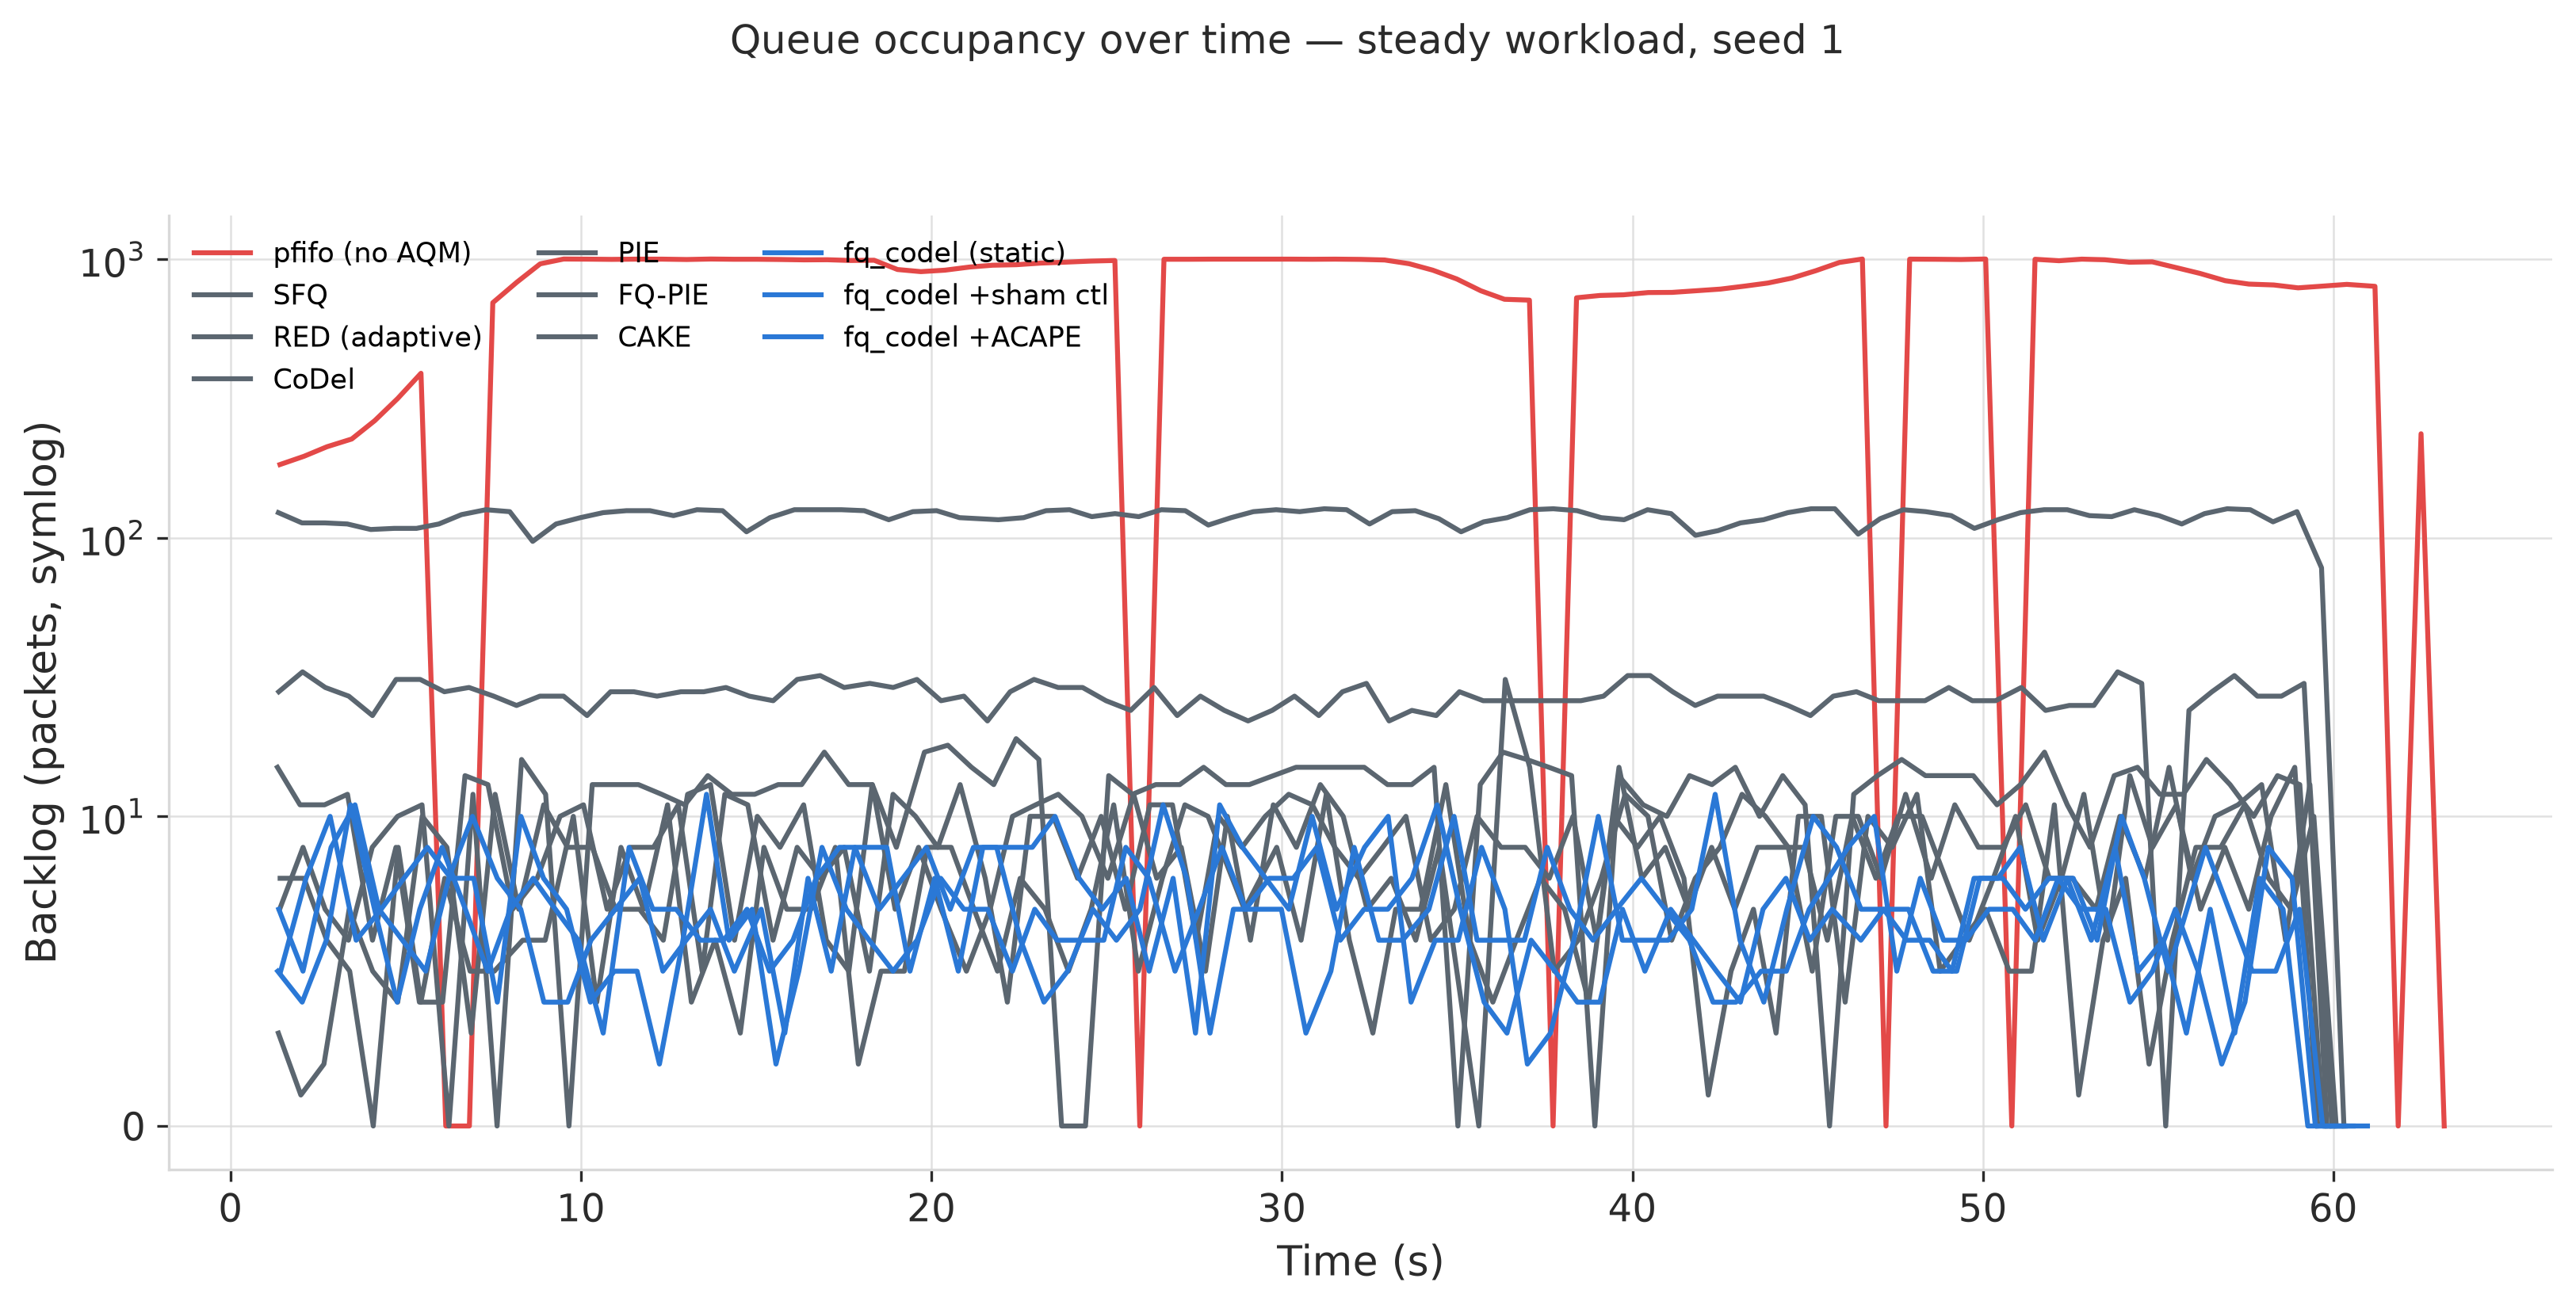
\includegraphics[width=\linewidth,height=0.42\textheight,keepaspectratio]{fig10_timeseries_backlog_steady.png}
\caption{\textbf{FIG 30}: fig10\_timeseries\_backlog\_steady.png. Queue occupancy over time (steady workload)}
\end{figure}

\begin{figure}[htbp]
\centering
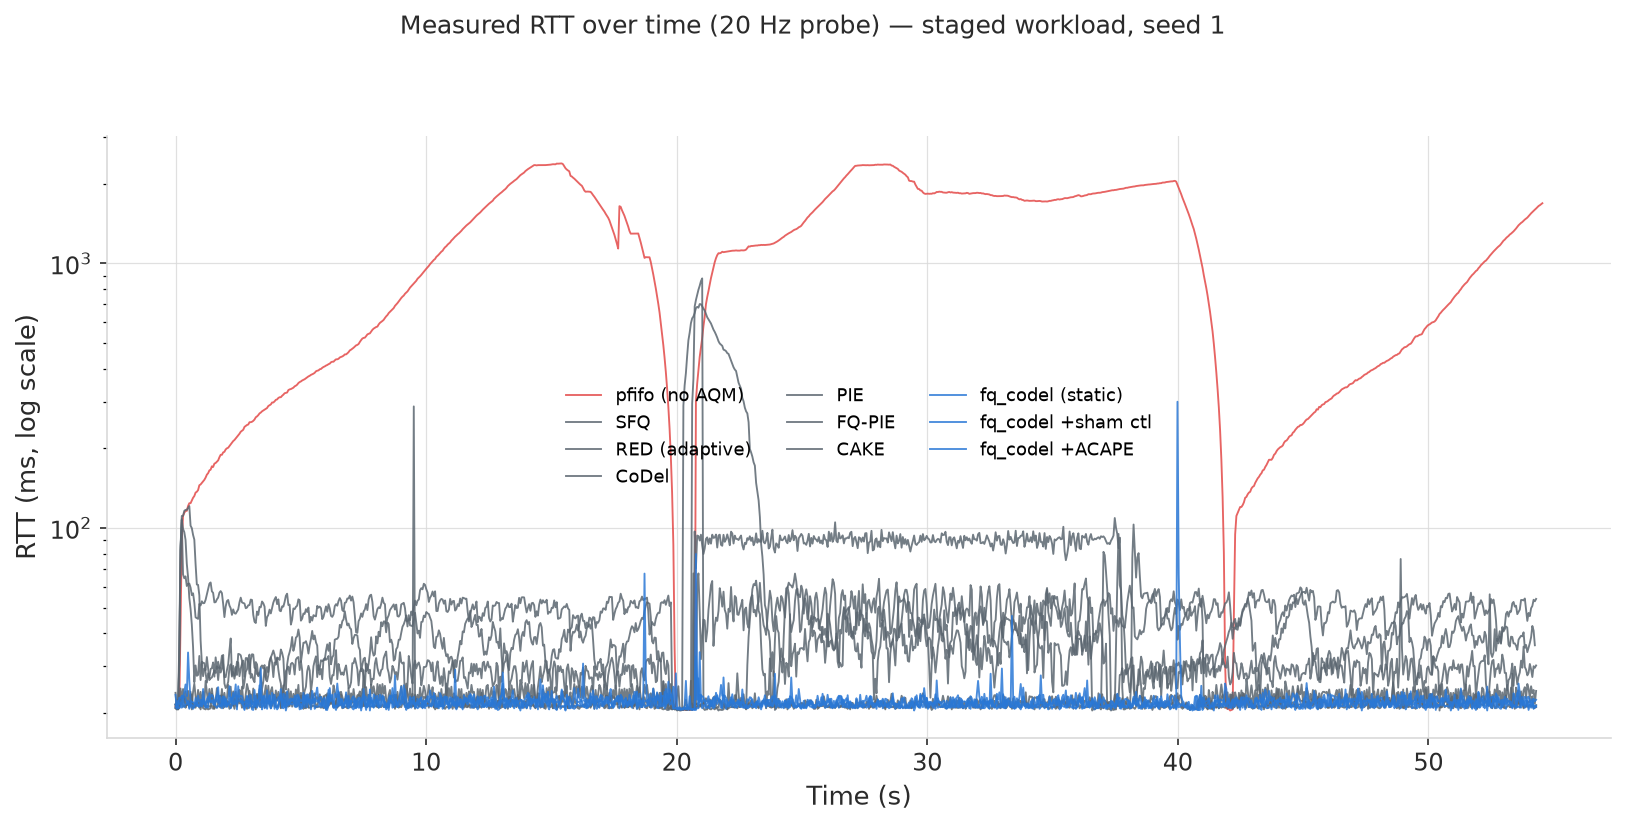
\includegraphics[width=\linewidth,height=0.42\textheight,keepaspectratio]{fig11_timeseries_rtt_staged.png}
\caption{\textbf{FIG 31}: fig11\_timeseries\_rtt\_staged.png. Measured RTT over time (20 Hz probe) (staged workload)}
\end{figure}

\begin{figure}[htbp]
\centering
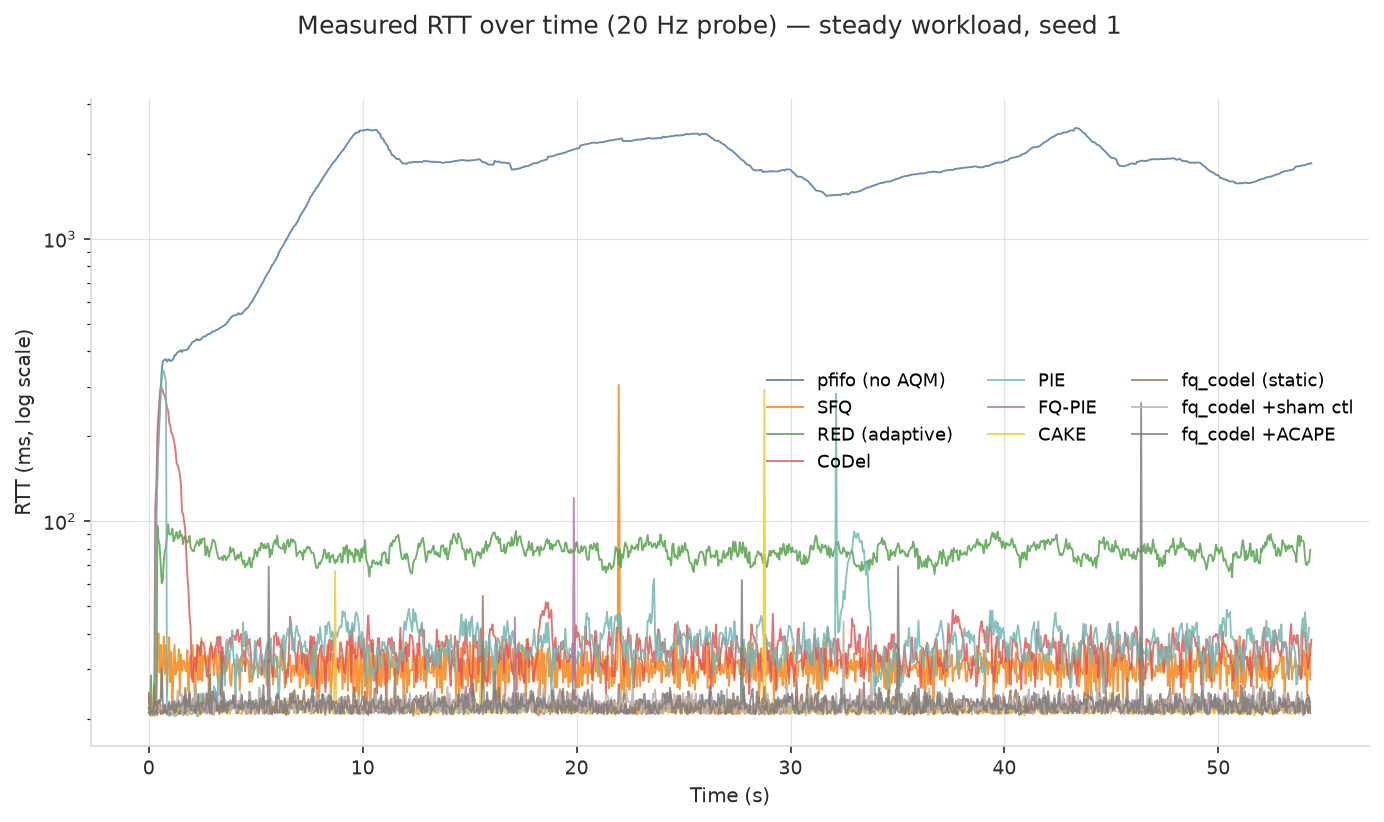
\includegraphics[width=\linewidth,height=0.42\textheight,keepaspectratio]{fig11_timeseries_rtt_steady.png}
\caption{\textbf{FIG 32}: fig11\_timeseries\_rtt\_steady.png. Measured RTT over time (20 Hz probe) (steady workload)}
\end{figure}

\begin{figure}[htbp]
\centering
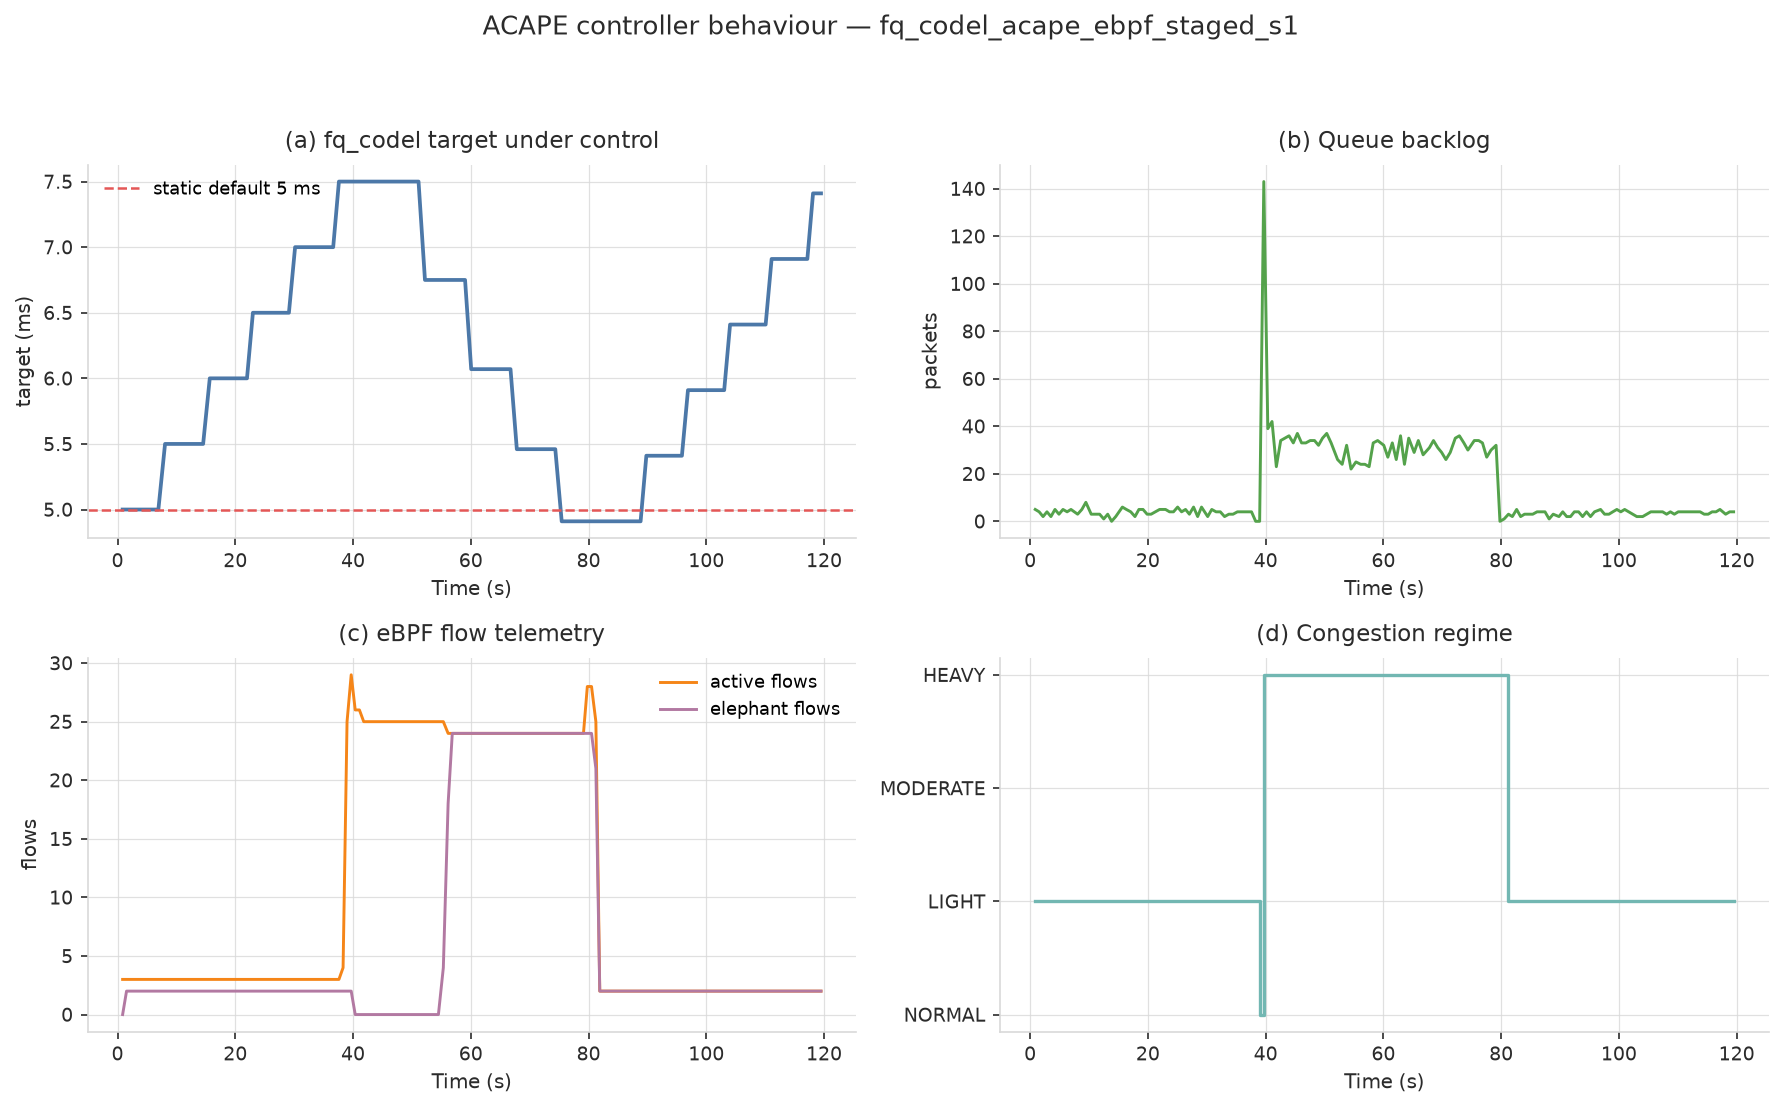
\includegraphics[width=\linewidth,height=0.42\textheight,keepaspectratio]{fig12_controller_behaviour.png}
\caption{\textbf{FIG 33}: fig12\_controller\_behaviour.png. What the ACAPE controller actually did: target, backlog, eBPF telemetry, regime}
\end{figure}

\begin{figure}[htbp]
\centering
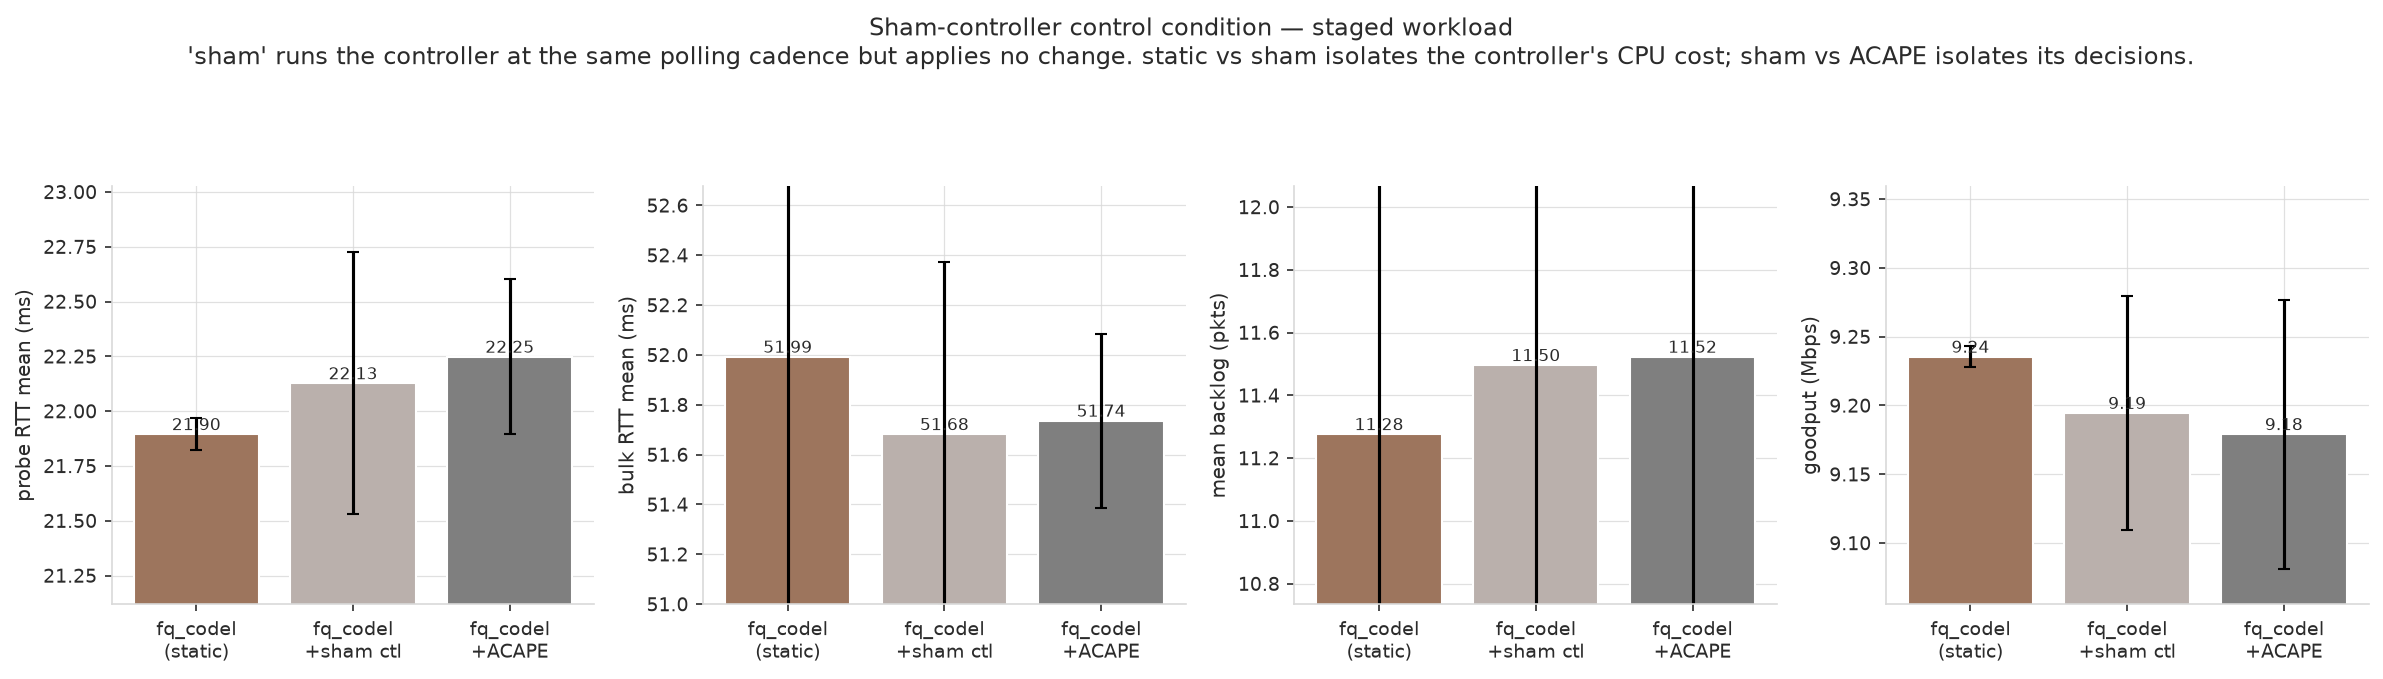
\includegraphics[width=\linewidth,height=0.42\textheight,keepaspectratio]{fig13_sham_control_staged.png}
\caption{\textbf{FIG 34}: fig13\_sham\_control\_staged.png. Sham-controller condition ,  separates controller CPU cost from control decisions (staged workload)}
\end{figure}

\begin{figure}[htbp]
\centering
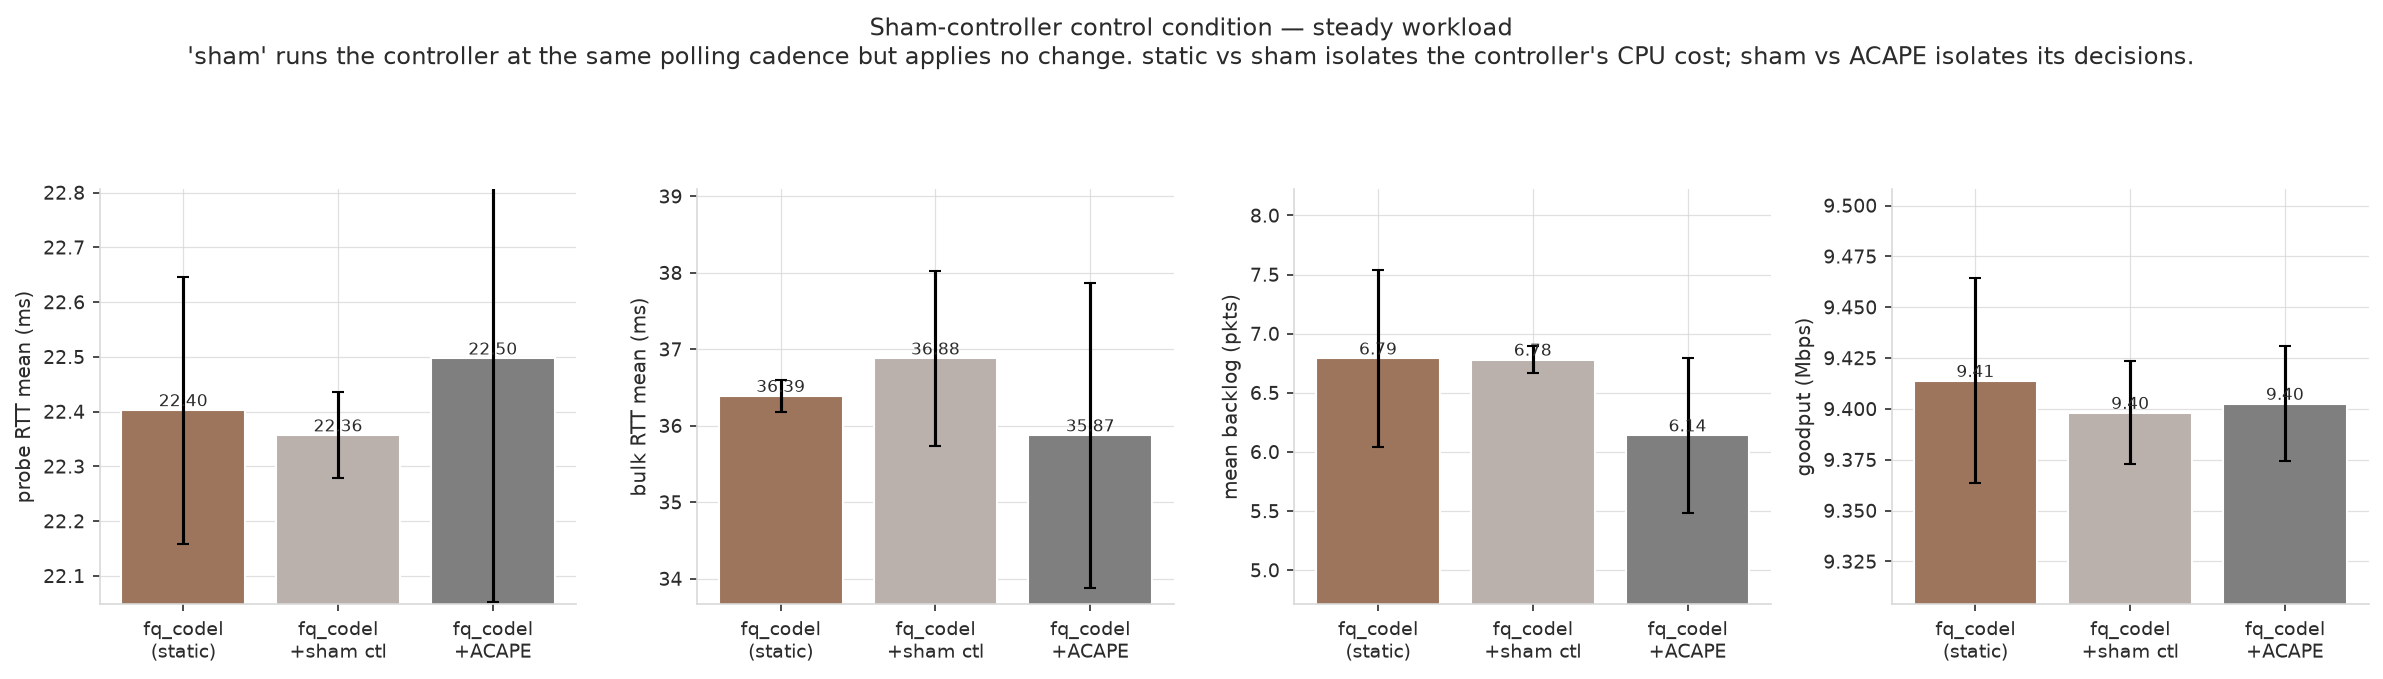
\includegraphics[width=\linewidth,height=0.42\textheight,keepaspectratio]{fig13_sham_control_steady.png}
\caption{\textbf{FIG 35}: fig13\_sham\_control\_steady.png. Sham-controller condition ,  separates controller CPU cost from control decisions (steady workload)}
\end{figure}

\clearpage
\section{Per-run figures}

One figure per experimental run, 63 in total, each showing that run's
time series. They are listed here rather than embedded, since the analysis
figures above aggregate them and the per-run detail is for checking a
specific run rather than for reading through. Every file is in
\texttt{figures/runs/} in the repository.


\begin{longtable}{p{1.6cm}p{5.2cm}p{7.6cm}}
\toprule ID & Run & Summary \\ \midrule
\endfirsthead
\toprule ID & Run & Summary \\ \midrule
\endhead
RUN 01 & \texttt{cake\_staged\_s1} & cake, staged workload, seed 1 ,  goodput 9.1985 Mbps, p95 RTT 22.2 ms, backlog 8.92 pkt \\
RUN 02 & \texttt{cake\_staged\_s2} & cake, staged workload, seed 2 ,  goodput 9.2728 Mbps, p95 RTT 22.3 ms, backlog 11.2 pkt \\
RUN 03 & \texttt{cake\_staged\_s3} & cake, staged workload, seed 3 ,  goodput 9.25 Mbps, p95 RTT 22.3 ms, backlog 11.28 pkt \\
RUN 04 & \texttt{cake\_steady\_s1} & cake, steady workload, seed 1 ,  goodput 9.4098 Mbps, p95 RTT 22.8 ms, backlog 6.89 pkt \\
RUN 05 & \texttt{cake\_steady\_s2} & cake, steady workload, seed 2 ,  goodput 9.4085 Mbps, p95 RTT 23.0 ms, backlog 6.55 pkt \\
RUN 06 & \texttt{cake\_steady\_s3} & cake, steady workload, seed 3 ,  goodput 9.4236 Mbps, p95 RTT 22.9 ms, backlog 6.58 pkt \\
RUN 07 & \texttt{codel\_staged\_s1} & codel, staged workload, seed 1 ,  goodput 9.2517 Mbps, p95 RTT 193.0 ms, backlog 23.58 pkt \\
RUN 08 & \texttt{codel\_staged\_s2} & codel, staged workload, seed 2 ,  goodput 9.2975 Mbps, p95 RTT 126.0 ms, backlog 23.71 pkt \\
RUN 09 & \texttt{codel\_staged\_s3} & codel, staged workload, seed 3 ,  goodput 9.2825 Mbps, p95 RTT 197.0 ms, backlog 25.09 pkt \\
RUN 10 & \texttt{codel\_steady\_s1} & codel, steady workload, seed 1 ,  goodput 9.4456 Mbps, p95 RTT 43.7 ms, backlog 8.98 pkt \\
RUN 11 & \texttt{codel\_steady\_s2} & codel, steady workload, seed 2 ,  goodput 9.445 Mbps, p95 RTT 46.7 ms, backlog 8.63 pkt \\
RUN 12 & \texttt{codel\_steady\_s3} & codel, steady workload, seed 3 ,  goodput 9.4614 Mbps, p95 RTT 44.9 ms, backlog 8.04 pkt \\
RUN 13 & \texttt{fq\_codel\_acape\_ebpf\_staged\_s1} & fq\_codel + ACAPE + eBPF, staged workload, seed 1 ,  goodput None Mbps, p95 RTT 24.7 ms, backlog 11.19 pkt \\
RUN 14 & \texttt{fq\_codel\_acape\_ebpf\_staged\_s2} & fq\_codel + ACAPE + eBPF, staged workload, seed 2 ,  goodput None Mbps, p95 RTT 25.3 ms, backlog 11.93 pkt \\
RUN 15 & \texttt{fq\_codel\_acape\_ebpf\_staged\_s3} & fq\_codel + ACAPE + eBPF, staged workload, seed 3 ,  goodput None Mbps, p95 RTT 24.5 ms, backlog 12.96 pkt \\
RUN 16 & \texttt{fq\_codel\_acape\_staged\_s1} & fq\_codel + ACAPE, staged workload, seed 1 ,  goodput 9.1339 Mbps, p95 RTT 23.5 ms, backlog 12.5 pkt \\
RUN 17 & \texttt{fq\_codel\_acape\_staged\_s2} & fq\_codel + ACAPE, staged workload, seed 2 ,  goodput 9.1986 Mbps, p95 RTT 23.3 ms, backlog 10.4 pkt \\
RUN 18 & \texttt{fq\_codel\_acape\_staged\_s3} & fq\_codel + ACAPE, staged workload, seed 3 ,  goodput 9.2051 Mbps, p95 RTT 23.6 ms, backlog 10.16 pkt \\
RUN 19 & \texttt{fq\_codel\_acape\_steady\_s1} & fq\_codel + ACAPE, steady workload, seed 1 ,  goodput 9.3894 Mbps, p95 RTT 24.5 ms, backlog 6.34 pkt \\
RUN 20 & \texttt{fq\_codel\_acape\_steady\_s2} & fq\_codel + ACAPE, steady workload, seed 2 ,  goodput 9.4088 Mbps, p95 RTT 24.4 ms, backlog 5.84 pkt \\
RUN 21 & \texttt{fq\_codel\_acape\_steady\_s3} & fq\_codel + ACAPE, steady workload, seed 3 ,  goodput 9.4093 Mbps, p95 RTT 24.4 ms, backlog 6.24 pkt \\
RUN 22 & \texttt{fq\_codel\_sham\_staged\_s1} & fq\_codel, staged workload, seed 1 ,  goodput 9.1858 Mbps, p95 RTT 23.6 ms, backlog 11.93 pkt \\
RUN 23 & \texttt{fq\_codel\_sham\_staged\_s2} & fq\_codel, staged workload, seed 2 ,  goodput 9.2323 Mbps, p95 RTT 23.5 ms, backlog 10.3 pkt \\
RUN 24 & \texttt{fq\_codel\_sham\_staged\_s3} & fq\_codel, staged workload, seed 3 ,  goodput 9.1657 Mbps, p95 RTT 23.4 ms, backlog 12.26 pkt \\
RUN 25 & \texttt{fq\_codel\_sham\_steady\_s1} & fq\_codel, steady workload, seed 1 ,  goodput 9.4098 Mbps, p95 RTT 24.6 ms, backlog 6.82 pkt \\
RUN 26 & \texttt{fq\_codel\_sham\_steady\_s2} & fq\_codel, steady workload, seed 2 ,  goodput 9.3923 Mbps, p95 RTT 24.6 ms, backlog 6.73 pkt \\
RUN 27 & \texttt{fq\_codel\_sham\_steady\_s3} & fq\_codel, steady workload, seed 3 ,  goodput 9.392 Mbps, p95 RTT 24.5 ms, backlog 6.79 pkt \\
RUN 28 & \texttt{fq\_codel\_staged\_s1} & fq\_codel, staged workload, seed 1 ,  goodput 9.232 Mbps, p95 RTT 23.3 ms, backlog 11.15 pkt \\
RUN 29 & \texttt{fq\_codel\_staged\_s2} & fq\_codel, staged workload, seed 2 ,  goodput 9.2362 Mbps, p95 RTT 23.4 ms, backlog 11.8 pkt \\
RUN 30 & \texttt{fq\_codel\_staged\_s3} & fq\_codel, staged workload, seed 3 ,  goodput 9.2382 Mbps, p95 RTT 23.5 ms, backlog 10.88 pkt \\
RUN 31 & \texttt{fq\_codel\_steady\_s1} & fq\_codel, steady workload, seed 1 ,  goodput 9.3904 Mbps, p95 RTT 24.6 ms, backlog 6.47 pkt \\
RUN 32 & \texttt{fq\_codel\_steady\_s2} & fq\_codel, steady workload, seed 2 ,  goodput 9.4243 Mbps, p95 RTT 24.6 ms, backlog 6.83 pkt \\
RUN 33 & \texttt{fq\_codel\_steady\_s3} & fq\_codel, steady workload, seed 3 ,  goodput 9.4266 Mbps, p95 RTT 24.5 ms, backlog 7.07 pkt \\
RUN 34 & \texttt{fq\_pie\_staged\_s1} & fq\_pie, staged workload, seed 1 ,  goodput 9.2375 Mbps, p95 RTT 23.3 ms, backlog 18.24 pkt \\
RUN 35 & \texttt{fq\_pie\_staged\_s2} & fq\_pie, staged workload, seed 2 ,  goodput 9.1944 Mbps, p95 RTT 23.2 ms, backlog 18.87 pkt \\
RUN 36 & \texttt{fq\_pie\_staged\_s3} & fq\_pie, staged workload, seed 3 ,  goodput 9.2358 Mbps, p95 RTT 23.2 ms, backlog 18.71 pkt \\
RUN 37 & \texttt{fq\_pie\_steady\_s1} & fq\_pie, steady workload, seed 1 ,  goodput 9.4285 Mbps, p95 RTT 23.3 ms, backlog 11.62 pkt \\
RUN 38 & \texttt{fq\_pie\_steady\_s2} & fq\_pie, steady workload, seed 2 ,  goodput 9.4996 Mbps, p95 RTT 23.2 ms, backlog 12.73 pkt \\
RUN 39 & \texttt{fq\_pie\_steady\_s3} & fq\_pie, steady workload, seed 3 ,  goodput 9.4297 Mbps, p95 RTT 23.3 ms, backlog 11.47 pkt \\
RUN 40 & \texttt{pfifo\_staged\_s1} & pfifo, staged workload, seed 1 ,  goodput 8.5918 Mbps, p95 RTT 2339.0 ms, backlog 564.36 pkt \\
RUN 41 & \texttt{pfifo\_staged\_s2} & pfifo, staged workload, seed 2 ,  goodput 8.303 Mbps, p95 RTT 2300.0 ms, backlog 558.08 pkt \\
RUN 42 & \texttt{pfifo\_staged\_s3} & pfifo, staged workload, seed 3 ,  goodput 8.2458 Mbps, p95 RTT 2315.0 ms, backlog 588.19 pkt \\
RUN 43 & \texttt{pfifo\_steady\_s1} & pfifo, steady workload, seed 1 ,  goodput 9.4101 Mbps, p95 RTT 2359.0 ms, backlog 778.62 pkt \\
RUN 44 & \texttt{pfifo\_steady\_s2} & pfifo, steady workload, seed 2 ,  goodput 9.4736 Mbps, p95 RTT 2339.0 ms, backlog 793.82 pkt \\
RUN 45 & \texttt{pfifo\_steady\_s3} & pfifo, steady workload, seed 3 ,  goodput 9.4757 Mbps, p95 RTT 2334.0 ms, backlog 795.29 pkt \\
RUN 46 & \texttt{pie\_staged\_s1} & pie, staged workload, seed 1 ,  goodput 9.1959 Mbps, p95 RTT 51.0 ms, backlog 10.75 pkt \\
RUN 47 & \texttt{pie\_staged\_s2} & pie, staged workload, seed 2 ,  goodput 9.2418 Mbps, p95 RTT 47.8 ms, backlog 10.0 pkt \\
RUN 48 & \texttt{pie\_staged\_s3} & pie, staged workload, seed 3 ,  goodput 9.2322 Mbps, p95 RTT 46.9 ms, backlog 10.24 pkt \\
RUN 49 & \texttt{pie\_steady\_s1} & pie, steady workload, seed 1 ,  goodput 9.406 Mbps, p95 RTT 47.4 ms, backlog 8.7 pkt \\
RUN 50 & \texttt{pie\_steady\_s2} & pie, steady workload, seed 2 ,  goodput 9.4254 Mbps, p95 RTT 47.2 ms, backlog 8.77 pkt \\
RUN 51 & \texttt{pie\_steady\_s3} & pie, steady workload, seed 3 ,  goodput 9.4072 Mbps, p95 RTT 46.2 ms, backlog 9.05 pkt \\
RUN 52 & \texttt{red\_staged\_s1} & red, staged workload, seed 1 ,  goodput 9.2535 Mbps, p95 RTT 94.2 ms, backlog 21.39 pkt \\
RUN 53 & \texttt{red\_staged\_s2} & red, staged workload, seed 2 ,  goodput 9.1977 Mbps, p95 RTT 94.0 ms, backlog 22.31 pkt \\
RUN 54 & \texttt{red\_staged\_s3} & red, staged workload, seed 3 ,  goodput 9.2849 Mbps, p95 RTT 94.3 ms, backlog 21.73 pkt \\
RUN 55 & \texttt{red\_steady\_s1} & red, steady workload, seed 1 ,  goodput 9.4726 Mbps, p95 RTT 87.3 ms, backlog 26.57 pkt \\
RUN 56 & \texttt{red\_steady\_s2} & red, steady workload, seed 2 ,  goodput 9.3863 Mbps, p95 RTT 88.3 ms, backlog 26.63 pkt \\
RUN 57 & \texttt{red\_steady\_s3} & red, steady workload, seed 3 ,  goodput 9.4894 Mbps, p95 RTT 86.5 ms, backlog 26.85 pkt \\
RUN 58 & \texttt{sfq\_staged\_s1} & sfq, staged workload, seed 1 ,  goodput 9.1821 Mbps, p95 RTT 57.4 ms, backlog 96.93 pkt \\
RUN 59 & \texttt{sfq\_staged\_s2} & sfq, staged workload, seed 2 ,  goodput 9.4066 Mbps, p95 RTT 55.0 ms, backlog 92.86 pkt \\
RUN 60 & \texttt{sfq\_staged\_s3} & sfq, staged workload, seed 3 ,  goodput 9.1979 Mbps, p95 RTT 57.4 ms, backlog 99.79 pkt \\
RUN 61 & \texttt{sfq\_steady\_s1} & sfq, steady workload, seed 1 ,  goodput 9.3558 Mbps, p95 RTT 36.2 ms, backlog 117.58 pkt \\
RUN 62 & \texttt{sfq\_steady\_s2} & sfq, steady workload, seed 2 ,  goodput 9.3542 Mbps, p95 RTT 36.1 ms, backlog 115.49 pkt \\
RUN 63 & \texttt{sfq\_steady\_s3} & sfq, steady workload, seed 3 ,  goodput 9.4238 Mbps, p95 RTT 36.0 ms, backlog 116.42 pkt \\
\bottomrule
\end{longtable}

\section{Where the numbers come from}

Every quantity in the paper and in this report is produced by the analysis
pipeline and read into \LaTeX{} as a generated macro, so prose cannot drift
from data. To regenerate everything from the committed logs:

\begin{verbatim}
python3 src/analyse.py          # tables, fact macros
python3 src/analyse_law.py      # the scaling law, its table and macros
python3 src/plots.py            # all analysis figures
python3 src/make_index.py       # the figure index this report is built from
python3 paper/make_report.py    # this document
\end{verbatim}

\noindent
The measurement defects found and corrected during the work, including the
four that would have decided the scaling-law result rather than measuring it,
are documented in the \texttt{verification/} directory. The pre-registered
hypotheses and their decision thresholds, committed before the data existed,
are in \texttt{docs/SCALING\_LAW.md}, \texttt{docs/CROSS\_AQM\_PREREG.md},
\texttt{docs/SERIALIZATION\_PREREG.md} and \texttt{docs/GATE\_PREREG.md}.

\end{document}
